%%%%%%%%%%%%%%%%%%%%%%%%%%%%%%%%%%%%%%%%%
% Masters/Doctoral Thesis 
% LaTeX Template
% Version 2.5 (27/8/17)
%
% This template was downloaded from:
% http://www.LaTeXTemplates.com
%
% Version 2.x major modifications by:
% Vel (vel@latextemplates.com)
%
% This template is based on a template by:
% Steve Gunn (http://users.ecs.soton.ac.uk/srg/softwaretools/document/templates/)
% Sunil Patel (http://www.sunilpatel.co.uk/thesis-template/)
%
% Template license:
% CC BY-NC-SA 3.0 (http://creativecommons.org/licenses/by-nc-sa/3.0/)
%
%%%%%%%%%%%%%%%%%%%%%%%%%%%%%%%%%%%%%%%%%

%----------------------------------------------------------------------------------------
%	PACKAGES AND OTHER DOCUMENT CONFIGURATIONS
%----------------------------------------------------------------------------------------

\documentclass[
11pt, % The default document font size, options: 10pt, 11pt, 12pt
%oneside, % Two side (alternating margins) for binding by default, uncomment to switch to one side
english, % ngerman for German
doublespacing, % Single line spacing, alternatives: onehalfspacing or doublespacing
%draft, % Uncomment to enable draft mode (no pictures, no links, overfull hboxes indicated)
nolistspacing, % If the document is onehalfspacing or doublespacing, uncomment this to set spacing in lists to single
%liststotoc, % Uncomment to add the list of figures/tables/etc to the table of contents
%toctotoc, % Uncomment to add the main table of contents to the table of contents
%parskip, % Uncomment to add space between paragraphs
%nohyperref, % Uncomment to not load the hyperref package
headsepline, % Uncomment to get a line under the header
%chapterinoneline, % Uncomment to place the chapter title next to the number on one line
consistentlayout, % Uncomment to change the layout of the declaration, abstract and acknowledgements pages to match the default layout
]{MastersDoctoralThesis} % The class file specifying the document structure

\usepackage[utf8]{inputenc} % Required for inputting international characters
\usepackage[T1]{fontenc} % Output font encoding for international characters
\usepackage{mathpazo} % Use the Palatino font by default
\usepackage[backend=biber,style=apa,natbib=true, maxcitenames=2]{biblatex} % Use the biber backend with the APA citation style
\usepackage{tabularx} % For wide tables
\usepackage{chngpage} % temporary change margins
\usepackage{booktabs} % nicer tables: % just makes the table prettier (see \toprule, \bottomrule, etc. commands below)
\usepackage{caption} % table caption width fitting table width
\usepackage{graphicx} % import pdf as graphics
\usepackage{float} % for better floating
\renewcommand\floatpagefraction{0}
\usepackage{threeparttable} % for caption and foot notes matching textwidth
\usepackage{ragged2e} % for left align caption:  \captionsetup{justification=RaggedRight}
\usepackage{pdfpages} % for inserting pdf documents
\usepackage{multirow} % multiple rows cell in tables
\usepackage{hyperref}% adding hyperlinks in document
\hypersetup{allcolors=blue}
\addbibresource{thesis.bib} % The filename of the bibliography
\usepackage[autostyle=true]{csquotes} % Required to generate language-dependent quotes in the bibliography
\usepackage[version=4]{mhchem} % used for easy presentation of Chemical structures
\usepackage{textgreek} %used for greek alphabet to be used in text mode
\usepackage{lipsum} %  Lorem Ipsum dummy text generator
\usepackage{lscape} % Table in landscape format
\usepackage{longtable} % multi page tables
\usepackage{array} % top align cell text in longtable
\usepackage[export]{adjustbox} % extra large figures via \includegraphics[max size={\textwidth}{\textheight}]{images/eiffel_tower}
\usepackage{placeins} %\ FloatBarrier
\usepackage{afterpage} % no emptypage after floatbarrier
 \usepackage{tocloft} % Add list of figures and tables as section within a chapter
\usepackage{tabto} % TAB like spaces
\usepackage{ragged2e} % For text alignment commands
\usepackage{microtype} 


%----------------------------------------------------------------------------------------
%	FUNCTIONS
%----------------------------------------------------------------------------------------

\newcommand{\insertFigure}[5]{%
  \vspace*{#4} % Vertikale Verschiebung
  \noindent
  \hspace*{#5} % Horizontale Verschiebung
  \includegraphics[page=#1, width=#2]{#3}
  \newpage
}
% invisible section header noticeable in the TOC
\makeatletter
\newcommand\invisiblesection[1]{%
  \refstepcounter{section}%
  \addcontentsline{toc}{section}{\protect\numberline{\thesection}#1}%
  \sectionmark{#1}\phantom{}}
\makeatother
% invisible subsection header noticeable in the TOC
\makeatletter
\newcommand\invisiblesubsection[1]{%
  \refstepcounter{subsection}%
  \addcontentsline{toc}{subsection}{\protect\numberline{\thesubsection}#1}%
  \sectionmark{#1}\phantom{}}
\makeatother

%----------------------------------------------------------------------------------------
%	MARGIN SETTINGS
%----------------------------------------------------------------------------------------

\geometry{
	paper=a4paper, % Change to letterpaper for US letter
	inner=2.5cm, % Inner margin
	outer=2.5cm, % Outer margin
	bindingoffset=0.5cm, % Binding offset
	top=1.5cm, % Top margin
	bottom=1.5cm, 
    head=21.89601pt,% Bottom margin
	%showframe, % Uncomment to show how the type block is set on the page
}

%----------------------------------------------------------------------------------------
%	THESIS INFORMATION
%----------------------------------------------------------------------------------------

\thesistitle{Aflatoxins in the Soil Environment --- Occurrence, Fate and Consequences for the Soil Microbiome and Associated Functions} % Your thesis title, this is used in the title and abstract, print it elsewhere with \ttitle
\supervisor{Dr. Katherine \textsc{Muñoz} \\ Prof. Dr. Gabriele E. \textsc{Schaumann}} % Your supervisor's name, this is used in the title page, print it elsewhere with \supname
\examiner{} % Your examiner's name, this is not currently used anywhere in the template, print it elsewhere with \examname
\degree{Doctor of Natural Sciences} % Your degree name, this is used in the title page and abstract, print it elsewhere with \degreename
\author{Julius \textsc{Albert}} % Your name, this is used in the title page and abstract, print it elsewhere with \authorname
\addresses{Neustadt an der Weinstraße, Deutschland} % Your address, this is not currently used anywhere in the template, print it elsewhere with \addressname

\subject{Environmental Sciences} % Your subject area, this is not currently used anywhere in the template, print it elsewhere with \subjectname
\keywords{} % Keywords for your thesis, this is not currently used anywhere in the template, print it elsewhere with \keywordnames
\university{{RPTU Rheinland-Pfälzische Technische Universität Kaiserslautern-Landau}} % Your university's name and URL, this is used in the title page and abstract, print it elsewhere with \univname
\department{\href{http://department.university.com}{Institute for Environmental Sciences}} % Your department's name and URL, this is used in the title page and abstract, print it elsewhere with \deptname
\group{\href{http://researchgroup.university.com}{Group of Environmental and Soil Chemistry}} % Your research group's name and URL, this is used in the title page, print it elsewhere with \groupname
\faculty{\href{http://faculty.university.com}{Faculty 7: Natural and Environmental Sciences}} % Your faculty's name and URL, this is used in the title page and abstract, print it elsewhere with \facname

\AtBeginDocument{
\hypersetup{pdftitle=\ttitle} % Set the PDF's title to your title
\hypersetup{pdfauthor=\authorname} % Set the PDF's author to your name
\hypersetup{pdfkeywords=\keywordnames} % Set the PDF's keywords to your keywords
}

%----------------------------------------------------------------------------------------
%%%%%%%%%%%%%%%%%%%%%%%%%%%%%%%%%%%%%%%%%%%%%%%%%%%%%%%%%%%%%%%%%%%%%%%%%%%%%%%%%%%%%%%%%
%   BEGIN DOCUMENT
%%%%%%%%%%%%%%%%%%%%%%%%%%%%%%%%%%%%%%%%%%%%%%%%%%%%%%%%%%%%%%%%%%%%%%%%%%%%%%%%%%%%%%%%%

\begin{document}

\frontmatter % Use roman page numbering style (i, ii, iii, iv...) for the pre-content pages

\pagestyle{plain} % Default to the plain heading style until the thesis style is called for the body content

%----------------------------------------------------------------------------------------
%	TITLE PAGE
%----------------------------------------------------------------------------------------

\begin{titlepage}
\begin{center}

\includegraphics[width=0.6\textwidth]{figures/logo_rptu.png}

\vspace*{.06\textheight}

\end{center}

\begin{center}
\onehalfspacing
\HRule \\[0.2cm] % Horizontal line
{\huge \bfseries \ttitle\par}\vspace{0.2cm} % Thesis title
\HRule \\[0.2cm] % Horizontal line
\vspace{1.2cm}
\end{center}

\begin{center}
{\LARGE \href{https://orcid.org/0000-0001-5468-6069}{\authorname}}

\vspace{1.2cm}

{\textsf{\large \textit{A thesis submitted in partial fulfillment of the requirements\\ for the degree of \degreename}}}

\vspace{1.5cm}
\vfill

{\textsf{Thesis examiners: \\
{Dr. Katherine \textsc{Muñoz}}\\
{Prof. Dr. Gabriele E. \textsc{Schaumann}}
}}

\vspace{0.8 cm}

\vfill

{\textsf{Faculty 7: Natural and Environmental Sciences\\
Institute for Environmental Sciences\\
University of Kaiserslautern--Landau}}

\vspace{1.2cm}

\vfill

{\Large \today}\\[4cm] % Date


\vfill

\end{center}
\end{titlepage}


%----------------------------------------------------------------------------------------
%	DECLARATION PAGE
%----------------------------------------------------------------------------------------

\begin{declaration}
\addchaptertocentry{\authorshipname} 

I hereby declare that this PhD thesis, entitled "Aflatoxins in the Soil Environment --- Occurrence, Fate and Consequences for the Soil Microbiome and Associated Functions”, was conducted and created by my own. All assistances, contributors and authors are declared and clearly indicated in this thesis. This PhD thesis has never been submitted elsewhere for an exam; neither to any other university nor to any other scientific institution. 

\noindent Place, Date:\\
\rule[0.5em]{25em}{0.5pt} % This prints a line for the signature
 
\noindent Signature:\\
\rule[0.5em]{25em}{0.5pt} % This prints a line to write the date
\end{declaration}
\let\cleardoublepage\clearpage

%----------------------------------------------------------------------------------------
%	PARTS OF THIS THESIS, AUTHOR CONTRIBUTIONS AND THIRD PARTY ASSISTANCES
%----------------------------------------------------------------------------------------

%----------------------------------------------------------------------------------------
\chapter*{Parts of this Thesis, Author Contributions and Third Party Assistances}
%----------------------------------------------------------------------------------------

This cumulative dissertation includes six chapters in which parts have been published as peer-reviewed research papers. In detail, Chapters 2, 4 and 5 are based on the respective accepted manuscripts, retaining their original formatting without any subsequent adjustments made. All research was conducted at the iES Landau, Institute for Environmental Sciences, at the University of Kaiserslautern--Landau (German: Rheinland--Pfälzische Technische Universität Kaiserslautern--Landau, also known as RPTU) in collaboration with the Kenya Agricultural and Livestock Research Organization (KALRO) for field sampling activities in Kenya. Financial support was provided by the project "AflaZ: Zero Aflatoxin" funded by the Federal Ministry of Food and Agriculture (BLE) under the reference AflaZ 2816PROC14. The subsequent section states the use of third party assistances and outlines the specific contributions made by both myself and the co-authors to the scientific work.

%----------------------------------------------------------------------------------------
\section*{Third Party assistances}
%----------------------------------------------------------------------------------------

In this thesis, the AI tools ChatGPT (version 3.5) and DeepL (Translator) were utilized in the writing process. Throughout the entire writing process, DeepL was used for translation purposes. The use of ChatGPT was confined to the Introduction (Chapter 1), the Kenyan field study (Chapter 3), and synthesis (Chapter 6) and was not involved in Chapters that were published in peer-reviewed journals, i.e., Chapter 2, 4, and 5. Its practical applications included serving as a tool for improving the overall quality of the text. Specifically, ChatGPT was utilized for tasks such as providing suggestions for phrasing and sentence structure, finding synonyms, acting as a grammar and spell-checker, and aiding in the concise summarization of content. ChatGPT supported the programming and formatting of LaTeX for the preparation of the thesis draft, especially for table formatting and the generation of BibTeX entries for the bibliography.

All figures in this dissertation were either created by the author or obtained from external sources with Creative Commons Zero (CC0) licenses, unless otherwise specified in the captions. The CC0-licensed cliparts and photos were sourced from freely available online databases, including Pexels, publicdomainvectors.org, Free-images.com, and Clker.com.

%----------------------------------------------------------------------------------------
\section*{Publications}
%----------------------------------------------------------------------------------------

The following chapters of this thesis have been published in peer-reviewed journals:

{\parindent2cm \hangindent\parindent\noindent\hbox to\parindent{\textbf{\textbf{Chapter 2}}\hfil}Albert, J., More, C. A., Dahlke, N. R., Steinmetz, Z., Schaumann, G. E., \& Muñoz, K. (2021). Validation of a Simple and Reliable Method for the Determination of Aflatoxins in Soil and Food Matrices. ACS omega, 6(29),  18684-18693. ISSN: 2470-1343. DOI: \href{https://pubs.acs.org/doi/10.1021/acsomega.1c01451}{10.1021/acsomega.1c01451}. \\[5pt]
\textit{Author contributions:}  J. Albert and K. Muñoz equally contributed to the conceptualization of the study and design of the experiments. The experiments were conducted by J. Albert, C. A. More, and N. R. P. Dahlke. J. Albert analyzed and visualized the data. J. Albert took the lead in writing and finalizing the manuscript. Project supervision was carried out by K. Muñoz and G. E. Schaumann. K. Muñoz was responsible for project administration and funding. The manuscript was finalized through contributions of all authors. \par} 

{\parindent2cm \hangindent\parindent\noindent\hbox to\parindent{\textbf{\textbf{Chapter 4}}\hfil}Albert, J., \& Muñoz, K. (2022). Kinetics of microbial and photochemical degradation of aflatoxin B1 in a sandy loam and clay soil. Scientific Reports, 12(1), 1684. ISSN: 2045-2322. DOI: \href{https://doi.org/10.1038/s41598-022-20727-1}{10.1038/s41598-022-20727-1}.\\[5pt]
\textit{Author contributions:}  J.A. designed the study, conceived the experiments, conducted data analysis, wrote and revised the manuscript; K.M. was involved in the study design, acquired funding, supervised the project and revised the manuscript. \par}


{\parindent2cm \hangindent\parindent\noindent\hbox to\parindent{\textbf{\textbf{Chapter 5}}\hfil}Albert, J., More, C., Korz, S., \& Muñoz, K. (2023). Soil Microbial Responses to Aflatoxin Exposure: Consequences for Biomass, Activity and Catabolic Functionality. Soil Systems, 7(1), 23. ISSN: 2571-8789. DOI: \href{https://doi.org/10.3390/soilsystems7010023}{10.3390/soilsystems-7010023}.\\[5pt]
\textit{Author contributions:} J. Albert and K. Muñoz were involved in the conceptualization of the study. Experiments were carried out by J. Albert, C. A. More, and S. Korz. Data analysis and visualization was carried out by J. Albert. J. Albert took lead in writing and finalizing the manuscript. K. Muñoz was responsible for project supervision, administration and funding. The manuscript was finalized through contributions of all authors. \par}

\hfill 

In addition to the publications listed above that represent Chapters of my thesis , I contributed to following publications. %\\

{\parindent2cm \hangindent\parindent\noindent\hbox to\parindent{\textbf{\textbf{Paper}}\hfil}Kenngott, K. G., Albert, J., Meyer-Wolfarth, F., Schaumann, G. E., \& Muñoz, K. (2022). Fusarium mycotoxins in maize field soils: method validation and implications for sampling strategy. Toxins, 14(2), 130. ISSN: 2072-6651. DOI: \href{https://doi.org/10.3390/toxins14020130}{10.3390/toxins14020130}.\\[5pt]
\textit{Author contributions:} Conceptualization was jointly undertaken by K. G. J. Kenngott, J. Albert, and K. Muñoz. Experiments were carried out by by K. G. J. Kenngott and J. Albert. Data analysis and visualization was carried out by K. G. J. Kenngott. K. G. J. Kenngott took lead in writing and finalizing the manuscript. Project supervision was carried out by  K. Muñoz and G. E. Schaumann. K. Muñoz was responsible for project administration and funding.
\par}

{\parindent2cm \hangindent\parindent\noindent\hbox to\parindent{\textbf{\textbf{Code}}\hfil} Steinmetz, Z., Albert, J., \& Kenngott, K. (2022). envalysis: Miscellaneous functions for environmental analyses. R Package Version 0.5.4. URL: \href{https://CRAN.R-project.org/package=envalysis}. DOI: \href{https://doi.org/ft9p}{ft9p}.\\[5pt] 
\textit{Author contributions:} Z. Steinmetz took the lead in setting up the package and programming and describing most of the functions. J. Albert provided code and description for the "matrix\_effect" function. J. Albert and K. G. J. Kenngott contributed to the coding and description of the "weight\_select" function. Z. Steinmetz was responsible for the maintenance of the package.
\par}
\clearpage

%----------------------------------------------------------------------------------------
%	QUOTATION PAGE
%----------------------------------------------------------------------------------------

\vspace*{0.2\textheight}

\noindent\enquote{\itshape You only know knowledge, you don't know the burning desire of will which only gives birth to knowledge.}\bigbreak

\hfill Leif Erikson, from "Conquerers of the Ocean" (Böttcher Straße in Bremen)
\clearpage

%----------------------------------------------------------------------------------------
%	ABSTRACT PAGE
%----------------------------------------------------------------------------------------

\begin{abstract}
\addchaptertocentry{\abstractname} % Add the abstract to the table of contents

Aflatoxins, a group of mycotoxins produced by various mold species within the genus \textit{Aspergillus}, have been extensively investigated for their potential to contaminate food and feed, rendering them unfit for consumption. Nevertheless, the role of aflatoxins as environmental contaminants in soil, which represents their natural habitat, remains a relatively unexplored area in aflatoxin research. This knowledge gap can be attributed, in part, to the methodological challenges associated with detecting aflatoxins in soil. The main objective of this PhD project was to develop and validate an analytical method that allows monitoring of aflatoxins in soil, and scrutinize the mechanisms and extent of occurrence of aflatoxins in soil, the processes governing their dissipation, and their impact on the soil microbiome and associated soil functions. By utilizing an efficient extraction solvent mixture comprising acetonitrile and water, coupled with an ultrasonication step, recoveries of 78\% to 92\% were achieved, enabling reliable determination of trace levels in soil ranging from 0.5 to 20 \textmu g kg\textsuperscript{-1}. However, in a field trial conducted in a high-risk model
region for aflatoxin contamination in Sub-Saharan Africa, no aflatoxins were detected using this procedure, underscoring the complexities of field monitoring. These challenges encompassed rapid degradation, spatial heterogeneity, and seasonal fluctuations in aflatoxin occurrence. Degradation experiments revealed the importance of microbial and photochemical processes in the dissipation of aflatoxins in soil with half-lives of 20 - 65 days. The rate of dissipation was found to be influenced by soil properties, most notably soil texture and the initial concentration of aflatoxins in the soil. An exposure study provided evidence that aflatoxins do not pose a substantial threat to the soil microbiome, encompassing microbial biomass, activity, and catabolic functionality. This was particularly evident in clayey soils, where the toxicity of aflatoxins diminished significantly due to their strong binding to clay minerals. However, several critical questions remain unanswered, emphasizing the necessity for further research to attain a more comprehensive understanding of the ecological importance of aflatoxins. Future research should prioritize the challenges associated with field monitoring of aflatoxins, elucidate the mechanisms responsible for the dissipation of aflatoxins in soil during microbial and photochemical degradation, and investigate the ecological consequences of aflatoxins in regions heavily affected by aflatoxins, taking into account the interactions between aflatoxins and environmental and anthropogenic stressors. Addressing these questions contributes to a comprehensive understanding of the environmental impact of aflatoxins in soil, ultimately contributing to more effective strategies for aflatoxin management in agriculture.


\end{abstract}
\clearpage

%----------------------------------------------------------------------------------------
%	ACKNOWLEDGEMENTS
%----------------------------------------------------------------------------------------

\begin{acknowledgements}
\addchaptertocentry{\acknowledgementname} % Add the acknowledgements to the table of contents
First and foremost, I would like to express my deepest gratitude to my advisor and mentor, Katherine Muñoz, for her unparalleled support and guidance during the difficult journey to complete my dissertation. I have always greatly appreciated and admired your exceptional and inspiring way of thinking, organizational skills, and tireless diligence. Our open exchange of ideas has always spurred me to new heights and inspired my thinking. You taught me to think, work and write scientifically. I am very grateful for your unwavering belief in my abilities and your willingness to let me work independently on my projects. Working with you has been a truly valuable experience, and I greatly appreciate the support you have given me during my doctoral studies. I extend my gratitude to Prof. Dr. Gabriele Ellen Schaumann, who co-supervised me and provided me with invaluable and uplifting feedback on my endeavors.


My thanks go to my my colleagues of our working group ‘Environmental and Soil Chemistry’, I thank you for your warm welcome, cooperativeness and support during the last years. My special thanks go to Camilla More, who has faithfully stood by my side throughout my doctoral studies. From the beginning of my doctoral studies, I had the honor and pleasure of supervising your bachelor thesis - a task that eventually made us not only valued colleagues, but also good friends. Over time, your role transformed from a student assistant during your bachelor program to an indispensable technical assistant and valued colleague. My special thanks to Angelika Holderle, who helped me through all administrative and organizational issues I had all theses years and for her open, gentle and helpful nature. I would also like to thank Zacharias Steinmetz, Kilian Kenngott, Christian Buchman, Maximiliam Meyer, and my other colleagues who have contributed to an invigorating and enjoyable work environment. Their constant support, insightful discussions, and camaraderie are truly appreciated. Furthermore, I want to thank our technical assistants, Karin Meyer, Silvia Eichhöfer, Anna Baskal and Andreas Hirsch for their support, skills and professional commitment in the laboratory that helped me many times during my experiments.


I extend my gratitude to all my student assistants and past bachelor's and master's students. A special mention goes to Sven Korz, Niklaus Dahlke, Kay Seufferheld, Sarah Morlock, Selina Morscheid, Maureen Roth, and Lisa Strotkötter. Their unwavering dedication and commendable efforts not only motivated me but also prompted me to revisit and refine my concepts. They consistently challenged me to elucidate intricate subjects in a comprehensible manner. Their contributions held significance, indirectly influencing my doctoral journey by providing crucial preliminary insights that laid the groundwork for planning and executing my main experiments. I value the commitment you demonstrated under my supervision, and it was a pleasure to work alongside you.


I also extend my gratitude to the collaborators of the AflaZ project, with special recognition to Markus Schmidt-Heydt and Christian Roder. Their dedication to managing and coordinating the project played a pivotal role in its inception and successful conclusion. Your positive and friendly demeanor greatly enriched my experience in the project. Furthermore, I'd like to express my appreciation to my project colleagues Christine Schwake-Anduschus, Wolfgang Büchs, Ronald Maul, and Torsten Meiners, as well as my fellow doctoral candidates, Alexandra Schamann, Ginson Riungu, and Beatrice Tenge. Our collaborative environment fostered by numerous meetings, conferences, and trips to Kenya created an enjoyable atmosphere. Lastly, special thanks go to our Kenyan project collaborators, particularly Charles Nkonge, Hillary Kibet Cheruiyot, and Ruth Amata. Your assistance and on-site support were essential, especially during the soil sampling in Kenya when travel restrictions due to the COVID-19 pandemic prevented my direct involvement. Your contributions were crucial in bringing this project to a successful conclusion.


Abschließend möchte ich meiner Familie, meinen Freunden und insbesondere meiner Freundin Lena von ganzem Herzen für ihre unermüdliche Geduld, Unterstützung und ständige Ermutigung während meiner Promotion danken. Eure Anwesenheit hat nicht nur meine Freude vervielfacht, sondern auch meine Entschlossenheit gestärkt. In den schwierigsten Momenten gaben mir die unterstützenden Gespräche und euer anhaltender Glaube an mich Kraft. Auch die ständigen Nachfragen über die Fortschritte meiner Dissertation haben mich motiviert und mich daran erinnert, dass ich auf diesem Weg nicht allein bin. Ohne euch wäre diese Arbeit in dieser Form nicht zustande gekommen. Ich bin froh, dass es euch gibt!


\end{acknowledgements}
\clearpage

%----------------------------------------------------------------------------------------
%	TABLE OF CONTENTS
%----------------------------------------------------------------------------------------

{
  \hypersetup{linkcolor=black}
  \tableofcontents
}

%----------------------------------------------------------------------------------------
%	THESIS CONTENT - CHAPTERS
%----------------------------------------------------------------------------------------

\mainmatter % Begin numeric (1,2,3...) page numbering
\pagestyle{thesis} % Return the page headers back to the "thesis" style

%########################################################################################
\chapter{Introduction} \label{Introduction} 
%########################################################################################

\clearpage

%========================================================================================
\section{Aflatoxins in the Food Production Chain} \label{subchap:AFs_introduction}
%========================================================================================

%----------------------------------------------------------------------------------------
\subsection{Aflatoxins: The Hidden Danger in Foods} \label{subchap:mycotoxins}
%----------------------------------------------------------------------------------------

Mycotoxins, produced as secondary metabolites by certain anamorphic fungal species, are natural contaminants in various food commodities, capable of causing disease and death in humans and animals upon consumption \citep{bennett2003clinical}. It is assumed that about 60 - 80\% of the global food crops are contaminated with mycotoxins \citep{eskola2020worldwide}. Roughly, more than a thousand mold species have been identified, of which more than 500 produce mycotoxins that have been classified as potentially toxic to vertebrates \citep{haque2020mycotoxin}. Major mycotoxins or groups of mycotoxins occuring in food that affect human and animal health include aflatoxins (AFs), ochratoxins, trichothecenes, fumonisins, alternariol, patulin and citrinin and alternaria toxins. These fungal toxins are produced by species within the genera \textit{Alternaria}, \textit{Aspergillus}, \textit{Fusarium} and \textit{Penicillium}. 


Aflatoxins (AFs), a group of mycotoxins that are produced by several species of the genus \textit{Aspergillus}, are widely considered as the most relevant mycotoxins from a food safety point of view due to their widespread occurence and high toxicity to humans \citep{afsah2013review, jallow2021worldwide}. To date, more than 20 aflatoxin molecules have been identified, with aflatoxin B1 (AFB1) exhibiting the highest toxicity to animals and humans \citep{ismail2018aflatoxin}. In addition to aflatoxin B1, the aflatoxins B2 (AFB2), G1 (AFG1), and G2 (AFG2),  as well as the derivative M1, which is primarily found in milk, are also of toxicological concern \citep{caceres2020aflatoxin, haque2020mycotoxin}. All aflatoxins are derivatives of dihydrofurancoumarins and share a common polycyclic structure derived from a coumarin nucleus linked to a bifurano system \citep{abrehame2023aflatoxins, nazhand2020characteristics}. They can be categorized into two chemical groups based on the binding to the dihydrofurancumarin structure: the difurocoumarocyclopentenone series (e.g., AFB1, AFB2, AFB2A, AFM1), characterized by the linkage to a pentanone ring, and the difurocoumarolactone series (e.g., AFG1, AFG2), characterized by the linkage to a lactone ring (Figure \ref{fig:Aflatoxins_structures_portrait}, \cite{abrehame2023aflatoxins, nazhand2020characteristics}). In addition, AFs can be further divided into AFs with (AFB1, AFB2, AFM1) and without (AFB2, AFG2, AFB2a) a double bond in the 8,9-position in the bifurano system \citep{abrehame2023aflatoxins}. 

%++++++++++++++++++++++++++++++++++++++++++++++++++++++++++++++++++++++++++++++++++++++++
\begin{figure}[ht!]
	\centering
	\includegraphics[width=1\textwidth]{figures/aflatoxins_structures_portrait.pdf}
	\decoRule
	\captionsetup{labelfont=bf, justification=justified, singlelinecheck=false, width=1\textwidth} 
	\caption{Structures of major important aflatoxins: aflatoxin B1 (AFB1), aflatoxin B2 (AFB2), aflatoxin B2a (AFB2a), aflatoxin G1 (AFG1), aflatoxin G2 (AFG2) and aflatoxin M1 (AFM1).}
	\label{fig:Aflatoxins_structures_portrait}
\end{figure}
%++++++++++++++++++++++++++++++++++++++++++++++++++++++++++++++++++++++++++++++++++++++++

%----------------------------------------------------------------------------------------
\subsection{Aflatoxin Occurrence in the Food Production Chain: Global Distribution and Geographical Variations} \label{subchap:occurence}
%----------------------------------------------------------------------------------------

Aflatoxin contamination is prevalent in various crops and regions worldwide, however, certain crops and conditions are more susceptible to AFs contamination. In general, oil- and starch-rich crops grown in (sub)tropical regions are the most susceptible to \textit{Aspergillus} infestation and aflatoxin contamination \citep{rushing2019aflatoxin, jallow2021worldwide}. Commodities that are frequently affected by aflatoxigenic fungi include cereals (wheat, sorghum, rice, acha, millet, guinea corn, corn), tree nuts (almond, pistachio, coconut, walnut), oilseeds (peanut, sunflower, cotton seeds, soybean, and sesame), spices (garlic, black pepper, coriander, turmeric, ginger, and chili peppers) \citep{awuchi2022mycotoxins}. The susceptibility of crops to fungal infestation and subsequent AFs production is influenced by a combination of environmental factors, crop-specific characteristics and the stage of food production chain and can already occurr "pre-harvest" in the field or "post-harvest" during storage, transport and processing (Figure \ref{fig:Food_chain}, \cite{jallow2021worldwide}).

%++++++++++++++++++++++++++++++++++++++++++++++++++++++++++++++++++++++++++++++++++++++++
\begin{figure}[ht]
	\centering
	\includegraphics[width=1\textwidth,center]{figures/food chain.jpg}
	\decoRule
	\captionsetup{labelfont=bf, justification=justified, singlelinecheck=false, width=1\textwidth}
	\caption{Factors influencing aflatoxin occurrence throughout the food and feed production chain from pre-harvest to post-harvest stages.}
	\label{fig:Food_chain}
\end{figure}
\afterpage{\FloatBarrier}
%++++++++++++++++++++++++++++++++++++++++++++++++++++++++++++++++++++++++++++++++++++++++

Fungal growth and aflatoxin production are determined by chemical (pH, oxygen, carbon dioxide, nutrient substrate composition, pesticides), physical (temperature, moisture, water activity, mechanical damage) and biological factors (plant variety, seed quality, plant physiology, stress, pest insects, presence of compatible toxigenic fungi, soil microbiome) \citep{pleadin2019mycotoxins, bryden2012mycotoxin}. In the field, these conditions are primarily determined by weather and site conditions, as well as agricultural practices such as weeding, fertilization, pest control, irrigation, tillage, and harvesting techniques (Figure \ref{fig:Food_chain}). Conditions favoring pre-harvest contamination of crops such as peanuts and maize are high temperatures, insect damage and prolonged drought conditions \citep{bryden2012mycotoxin}. During and post-harvest stage, proper crop handling and processing, including adequate drying, clean and dry storage, and protection from rodents and insects, has a significant impact on aflatoxin fungal formation conditions (Figure \ref{fig:Food_chain}, \cite{kyei2021awareness}).

%++++++++++++++++++++++++++++++++++++++++++++++++++++++++++++++++++++++++++++++++++++++++
\begin{figure}[ht]
	\centering
	\includegraphics[width=\textwidth,center]{figures/aflatoxin_prevalence.jpeg}
	\decoRule
	\captionsetup{labelfont=bf, justification=justified, singlelinecheck=false, width=\textwidth}
	\caption{World maps showing the prevalence of AFs (sum of AFB1, AFB2, AFG1 and AFG2) in feed samples: (a) Percentage of positive samples; (b) Number of samples exceeding 5 \textmu{}g kg\textsuperscript{-1}; (c) Number of samples exceeding 20 \textmu{}g kg\textsuperscript{-1}. Areas filled in grey indicate data not available. The data used for plotting is sourced from \citet{gruber2019global}.}
	\label{fig:Aflatoxin_Prevalence}
\end{figure}
\afterpage{\FloatBarrier}
%++++++++++++++++++++++++++++++++++++++++++++++++++++++++++++++++++++++++++++++++++++++++

Developing countries from the (sub)tropics are particularly confronted with aflatoxin food contamination, due to the favorable (sub)tropical conditions for the growth and aflatoxin formation of these fungi and the limited access to control measures \citep{gbashi2018socio, nji2022six}. In a study by \citet{gruber2019global}, about 75,000 feed samples collected from 100 countries from 2008 to 2017 were analyzed for mycotoxins, including aflatoxins. The results showed a clear tendency towards a higher AFs prevalence in Southeast Asia (57.4 \%), South Asia (82.2 \%) and Sub-Saharan Africa (76 \%) and a much lower prevalence in Northern (5.9 \%) and Central Europe (12.7 \%) (Figure~\ref{fig:Aflatoxin_Prevalence}). Likewise the the number of samples exceeding 5 and 20  \textmu{}g kg\textsuperscript{-1} AFs are much higher in Southeast Asia (37.9 and 20.9 \%),  South Asia (61.1 and 41.1 \%) and Sub-Saharan Africa (59.1 and 38.5 \%) than in Northern (2.4 and 0.4 \%) and Central Europe (2.6 and 1.0 \%), respectively (Figure~\ref{fig:Aflatoxin_Prevalence}). 


These favorable (sub)tropical conditions for aflatoxigenic fungi result not only in higher prevalence, but also in significantly higher aflatoxin levels in agricultural products. Table \ref{table:Aflatoxin_food_levels} (Chapter \ref{Annex_chap1}) shows the reported aflatoxin contamination levels for various food commodities from countries in different geographical regions, adapted from the compilations by \citet{jallow2021worldwide} and \citet{ismail2018aflatoxin}. Corn and peanuts, major staple foods grown in (sub)tropical regions, are often associated with particularly high levels of aflatoxins \citep{ismail2018aflatoxin}. For example \textSigma AFs levels in the range of 10 \textsuperscript{3} \textmu g kg\textsuperscript{-1} were reported for cereals and peanuts in Uganda \citep{sserumaga2020aflatoxin}, Congo \citep{kamika2016occurrence}, Ethiopia \citep{mohammed2016aspergillus}, Nigeria \citep{oyedele2017mycotoxin}, Kenya \citep{sirma2016aflatoxin}, China \citep{wu2016aflatoxin} and Tunisia \citep{houissa2019multimycotoxin}.
Spices can also exhibit high levels of contamination, reaching concentrations in this range, as observed in Lebano \citep{el2019multimycotoxins}. In rare cases, \textSigma AFs concentrations above 10000 \textmu g kg\textsuperscript{-1} can be detected, as for example in infant preparations from Mexico \citep{chala2013natural}. Furthermore, due to the importance of corn as animal feed - about 55\% of corn production is used for this purpose - there is a strong link to the presence of aflatoxins in dairy products \citep{tolosa2021multi}. For instance, AFM1 concentrations of up to 4.5 \textmu g L\textsuperscript{-1} have been detected in milk samples from Kenya \citep{kuboka2019occurrence}. These significantly elevated contamination levels mentioned above have profound impacts on both human health and international trade.

%----------------------------------------------------------------------------------------
\subsection{Consequences of Aflatoxins: From Human Exposure to Global Trade} \label{subchap:AFs_consequences}
%----------------------------------------------------------------------------------------

The aflatoxin contamination level in foods and feeds, as well as the rate of consumption of the local population, largely determine the extent of human exposure to aflatoxins and the associated health effects \citep{jallow2021worldwide}. The average intake of aflatoxins by humans is estimated to be 10 to 200 ng kg\textsuperscript{-1} day\textsuperscript{-1}, with a total range of 0 to 30,000 ng kg\textsuperscript{-1} day\textsuperscript{-1} \citep{kaplan2003clinical, gong2016aflatoxin}. Given the high production and consumption rates of staple crops such as corn and peanuts, coupled with a high susceptibility to aflatoxin contamination, these crops are the primary source through which humans are exposed to aflatoxins. It is therefore no coincidence that the highest aflatoxin exposure is consistently reported from developing countries in (sub)tropical regions \citep{jallow2021worldwide}. In this regard, approximately 4.5 billion people in the developing world are at risk of chronic, uncontrolled exposure to AFs \citep{williams2004human, rushing2019aflatoxin, shephard2003aflatoxin, williams2004human}. Particular high exposure levels are reported for Sub-Saharan Africa and South-East Asia \citep{gong2016aflatoxin} such as Kenya (3.5-14.8 ng kg\textsuperscript{-1} day\textsuperscript{-1}), Swaziland (11.4-158.6 ng kg\textsuperscript{-1} day\textsuperscript{-1}), Mozambique (38.6-183.7 ng kg\textsuperscript{-1} day\textsuperscript{-1}), South Africa (16.5 ng kg\textsuperscript{-1} day\textsuperscript{-1}), The Gambia (4-115 ng kg\textsuperscript{-1} day\textsuperscript{-1}), China (11.7-2027 ng kg\textsuperscript{-1} day\textsuperscript{-1}), and Thailand (6.5-53 ng kg\textsuperscript{-1} day\textsuperscript{-1}) \citep{williams2004human}. Meanwhile, exposure levels in developed countries are much lower e.g. 2.7 ng kg\textsuperscript{-1} day\textsuperscript{-1} in the USA \citep{williams2004human} and 0.93–2.45 ng kg\textsuperscript{-1} day\textsuperscript{-1} in Europe \citep{jecfa2008sixty}.


Elevated exposure levels are of particular concern because AFs are considered one of the most potent mutagenic and carcinogenic substances known to date \citep{eskola2020worldwide}. The International Agency for Research on Cancer classifies AFB1 and natural aflatoxin mixtures of B, G, and M aflatoxins as group 1 carcinogens \citep{IARC2006}. Aflatoxins exhibit a toxicity profile where AFB1 is the most potent, followed by AFM1, AFG1, AFB2, and AFG2, with demonstrated acute toxicological and chronic hepatocarcinogenic effects in the liver due to their reactivity with DNA, RNA, enzymes, and proteins \citep{haque2020mycotoxin}. Chronic aflatoxicosis has been linked to hepatocellular carcinoma or liver cancer, suppress growth, modulate the immune system, and lead to malnutrition \citep{rushing2019aflatoxin, IARC2006, haque2020mycotoxin}. In addition, aflatoxicosis can exhibit potent synergistic effects with other factors contributing to liver cancers, such as malnutrition and infection with hepatitis B and C viruses, diseases that are highly prevalent in developing countries -- conditions highly prevalent in developing countries, with hepatitis incidences reaching about 20\% \citep{williams2004human}. Meanwhile, acute aflatoxicosis has resulted in symptoms such as abdominal pain, vomiting and edema \citep{eskola2020worldwide}. Especially in developing countries in (sub)tropical regions such as Kenya, China, India and Malaysia with favorable conditions for the growth and aflatoxin production of these fungi and limited access to control measures such as safe food storage, severe outbreaks of AFB1 contamination in food frequently occur, resulting in hundreds of deaths from acute aflatoxicosis \citep{azziz2005case, eskola2020worldwide, haque2020mycotoxin}. 


The impact of aflatoxin contamination in agriculture extends beyond public health, affecting  trade and economics in both developed and developing countries \citep{jallow2021worldwide}. In this regard, maize farmers in the US lose \$160 million annually due to AFs contamination \citep{wu2015global}, but losses are higher in developing countries, especially in sub-Saharan Africa, where they reach losses of \$450 million, representing 38\% of global agricultural losses due to aflatoxin \citep{gbashi2018socio}. Aflatoxins also lead to a significant decrease in agricultural trade between developed and developing countries \citep{wu2015global}, in part due to the discrepancy between these countries in terms of regulatory limits on the one hand and the prevalence of AFs on the other. In general, AFs regulation in non-tropical and industrialized countries that are less affected by AF problems are much stricter than in tropical and developing countries that are in heavily affected \citep{sirma2018impacts}. This discrepancy creates several problems for tropical countries facing the AF problem, such as sub-Saharan Africa. In these countries, economies are predominantly based on the commercialization of agricultural products \citep{matumba2015concentrating}. The economic importance of agricultural production, combined with a high susceptibility to AFs contamination, has a significant impact on the trade and economy of developing countries in the tropics mainly by reducing the value of the commodities offered for sale \citep{jallow2021worldwide}, e.g. by lowering prices, inspection fees, disposal fees, rejecting or treating lots at extra cost, compensating for claims, and the cost of sampling and analysis in the supply chain \citep{gbashi2018socio}. Typically, the main staple foods in these countries are also their most important cash crops \citep{nji2022six}. As a result, the best-quality crops with the least contamination that meet the standards of non-tropical importing countries are usually exported, leaving the poorer quality, more contaminated crops for local consumption or sale in the informal sector \citep{matumba2015concentrating, nji2022six}. This increases the likelihood of the local population consuming AFs contaminated foods \citep{udomkun2017mycotoxins, nji2022six}, with result in further economic costs i.e. cost of illness \citep{meijer2021aflatoxin}.


Contaminated crops unsuitable for sale in the informal food sector or for in-house consumption are often spread in the field for surface decomposition or buried in the soil as organic fertilizer \citep{fouche2020aflatoxins}. However, the fate and consequences of AFs in soil and on soil organisms that provide important ecological services remain unclear \citep{fouche2020aflatoxins}. Consequently, AFs contamination could go beyond health and trade issues,  potentially affecting soil health, agricultural productivity and food safety.

%----------------------------------------------------------------------------------------
\subsection{Regulation of Aflatoxins in Foods and Feeds: Efforts at Local and Global Scales} \label{subchap:globalregulation}
%----------------------------------------------------------------------------------------

%++++++++++++++++++++++++++++++++++++++++++++++++++++++++++++++++++++++++++++++++++++++++
\begin{figure}[ht]
	\centering
	\includegraphics[width=1.15\textwidth,center]{figures/aflatoxin_regulation_limits.pdf}
	\decoRule
	\captionsetup{labelfont=bf, justification=justified, singlelinecheck=false, width=1.1\textwidth}
	\caption{World maps showing the regulation limits for AFB1 (a) and the sum of AFB1, AFB2, AFG1 and AFG2 (b) in maize and peanuts in the years 2002 and 2022. The polygons filled with a stripe pattern represent countries that have set limits for aflatoxin through international harmonized standards and those without a stripe pattern represent countries that have set their own national limits.}
	\label{fig:Aflatoxin_Regulation_Limits}
\end{figure} 
\afterpage{\FloatBarrier}
%++++++++++++++++++++++++++++++++++++++++++++++++++++++++++++++++++++++++++++++++++++++++

In order to protect humans and animals from the serious health effects of AFs, most countries have adopted strict regulations \citep{van2004worldwide}. Regulatory limits are established on sound risk assessments on the basis of toxicological and exposure data, as well as knowledge of the distribution of AFs concentrations within potentially susceptible commodities \citep{chilaka2022mycotoxin}. However, economic and political factors such as trade interests and adequate food supply also have an impact on the setting of local regulatory limits \citep{van2004worldwide}. In general, the maximum permissible values for AFs in foodstuffs are in the lower \textmu{}g kg\textsuperscript{-1} range \citep{van2004worldwide, sirma2018impacts}. In most countries, legal limits for the sum of the four major aflatoxins (AFB1, AFB2, AFG1 and AFG2) as well as the most toxic aflatoxin (AFB1) have been set at least for corn and peanuts due to their susceptibility and, at the same time, their importance as staple foods \citep{wu2013global}. A global survey conducted twenty years ago on behalf of the Food and Agriculture Organization of the United Nations (FAO) found that about 100 countries have specific regulations for AFs in various dairy products and feed items \citep{van2004worldwide}. The legal requirements differed strongly among the countries and regions (Figure~\ref{fig:Aflatoxin_Regulation_Limits}). While for Northern America, Southern America and Europe (inc. Russia) most countries implemented limits for AFB1 and/or the sum of AFs, there is a lack of regulation in Asian and African countries. Further, some free trade zones such as the EU, MERCOSUR, and Australia/New Zealand harmonized their limits. Although many countries do not have national or international legally binding limits for aflatoxins, it is important to know that many of these countries are members of the Codex Alimentarius Commission (CAC), which sets international standards, guidelines and codes of conduct to facilitate global trade and protect consumers. The CAC has established a standard for aflatoxins in peanuts (sum of AFs $\leq$ 15 \textmu{}g kg\textsuperscript{-1}), which, while not legally binding at the national level, can be considered a proxy regulation limit \citep{CAC1995}. A literature search on the situation of AF regulation in 2022 (Annex \ref{Annex_chap1}, Table~\ref{table:Aflatoxin_regulation}) revealed that an increasing number of countries have introduced limits either at national or internationally harmonized levels and that there is a general trend towards tightening AF limits, especially in African and Asian countries. By joining the European Union, several countries have adopted its particularly strict limits. Regionally harmonized aflatoxin limits have been introduced as a result of the formation of the Eurasian Customs Union (EACU), the East African Community (EAC), the African Organisation for Standardisation (ARSO) and the  Gulf Cooperation Council Standardization Organization (GSO). In addition, the number of Codex Alimentarius Commission member states increased between 2002 and 2022 from 168 to 189 (Figure~\ref{fig:Aflatoxin_Regulation_Limits}). Thus, the majority of countries in 2022 have some form of limits on AFs, either by setting national standards or by proxy. 


In non-tropical and developed countries where AF contamination is less prevalent, AF regulation levels are considerably more stringent compared to the regulations in tropical and developing nations, which are significantly more impacted by AF contamination \citep{sirma2018impacts}. For example, for the countries of the European Union the European Commission has defined some of the strictest limits with maximum permitted levels of 2 (AFB1) and 4 \textmu{}g kg\textsuperscript{-1} (sum AFB1, AFB2, AFG1, AFG2) and for maize and peanuts. On the other hand, the maximum levels set by the Ministry of Agriculture of the Republic of Indonesia are 15 (AFB1) and 20 \textmu{}g kg\textsuperscript{-1} (sum AFB1, AFB2, AFG1, AFG2) for maize and peanuts, respectively. These differences have significant implications for global trade and public health risks, as outlined in the previous chapter (Chapter \ref{subchap:AFs_consequences}). 


Current aflatoxin limits, designed primarily for formal markets, have limited ability to protect consumers in informal settings, particularly in subsistence agriculture, which is the predominant food production system in sub-Saharan Africa \citep{nji2022aflatoxins}. Therefore, it is important to take proactive measures to prevent aflatoxin contamination rather than relying solely on the effectiveness of limits. Such a preventive approach can protect consumers and effectively mitigate economic losses. Since AFs contamination can occur at various stages of the food production chain (Chapter \ref{subchap:occurence}), prevention include both pre- and post-harvest measures to ensure a comprehensive approach to controlling the risk of aflatoxin contamination.


%----------------------------------------------------------------------------------------
\subsection{Aflatoxin Prevention from Field to Fork: Integrated Approaches Along the Food Production Chain} \label{subchap:prevention}
%----------------------------------------------------------------------------------------

Aflatoxin control strategies rely on the knowledge of critical factors leading to increased growth and/or AF production of mold fungi (Figure \ref{fig:Food_chain}, Chapter \ref{subchap:occurence}). Based on sound experimental evidence, the Codex Alimentarius Comission has established several codes of practice for the prevention and mitigation of AF contamination in various crops, such as cereals \citep{CAC2003}, peanuts \citep{CAC2004}, tree nuts \citep{CAC2010}, figs \citep{CAC2008} and spices \citep{CAC2017} based on Good Agricultural Practice \citep{fao2003development}. These guidelines suggest management practices for all stages of the food production chain, including pre-harvest, harvesting and post-harvest stages.


In the pre-harvest stages, AF control strategies focus on improving plant health and impairing the growth and AF production of the fungi. The susceptibility of crops to fungal infection is closely related to their physiological condition, which can be influenced by various agricultural practices. The management practices recommended by the CAC to minimize AF contamination in the field can be summarized as follows: Use of certified seeds of resistant varieties that are free of toxic fungi, plowing under / destroying / removing of plant debris that may have served or potentially serves as substrate for aflatoxigenic fungi, timely planting to avoid heat and drought stress during seed development and maturation, avoidance of plant overcrowding by maintaining optimal plant densities, crop rotation, proper plant nutrition (fertilization and liming), avoiding drought stress (irrigation), controlling fungal vectors and plant pathogens including \textit{Asgergilli} and parasitic fungi other than \textit{Aspergilli} (fungicides), nematodes (nematocides), mites (acaricides), insects (insecticides) and weeds (herbicides). 


Recommended harvesting techniques are based on selecting harvesting conditions that reduce the risk of biological contamination. Firstly, appropriate harvest timing must be selected, which involves harvesting the crop when it has reached full maturity, ensuring acceptable moisture content, and prior to the onset of extreme weather conditions such as excessive heat, rainfall, or drought. In addition, functional and clean harvesting equipment should be used to allow timely harvesting, minimize physical damage to the harvested crop, and prevent the carryover of soil, dirt, dust, or contaminated plant material that could potentially serve as an inoculum for aflatoxigenic fungi. Any contact between the harvested crop and materials that may contain viable fungal structures should be avoided. Special attention should be paid to individual plants that have been damaged by pests or plant fractions with visible fungal contamination. These plants should be harvested separately to prevent rapid colonization by aflatoxigenic fungi during subsequent steps such as storage, transport and processing.


Post-harvest measures focus on preventing fungal invasion and/or creating conditions unsuitable for fungal growth and toxin formation. This includes avoiding piling, heaping, and storage of freshly harvested commodities with high moisture for extended periods of time. The crop should be dried as soon as possible after harvest in a manner that minimizes damage to the grain and maintains moisture levels lower than necessary for fungal growth during storage. In cases where immediate drying is not feasible, adequate aeration should be implemented. The drying, storage, and transport processes should take place in a clean, intact, protected, dry, and well-ventilated environment to protect the commodity against rain, dew, soil, pests, bird droppings, and other potential sources of contamination. Proper cleaning of the harvest is essential to remove damaged and immature plant material, as well as other foreign matter that may pose a risk of fungal infection. Continuous monitoring of the condition of stored and transported material is necessary to maintain acceptable temperature and moisture levels and minimize the presence of rodents and stored product pests, as these conditions can create favorable conditions for mold growth and AF production. The use of approved fumigants or insecticides may be appropriate for extended periods of transportation or storage.

Although soil is the natural habitat of AF producing fungi \citep{horn2003ecology, elmholt2008mycotoxins}, none of the proposed preventive measures specifically address soil as a conservation target. In fact, the impact of preventive measures on soil AF concentrations remains unknown. Certain actions, such as incorporation of plant residues by plowing, may potentially contribute to elevated AF input levels to soil \citep{fouche2020aflatoxins}.  Further, certain recommended management practices including fertilization, liming, irrigation, pesticide use can have negative effects on the integrity and functionality of the soil microbial communities \citep{tilman2002agricultural, sanaullah2020terrestrial}, potentially leading to changes in processes involved in the formation and dissipation of AFS. This, in turn, could affect the persistence of AFs in the soil and lead to ecological imbalances that potentially pose a threat to soil health. Therefore, soil has been largely neglected despite its central function in the context of AF prevention.



%========================================================================================
\section{Aflatoxins in the Soil Environment} \label{subchap:aflatoxins_in_soil}
%========================================================================================

%----------------------------------------------------------------------------------------
\subsection{Entry Pathways for Aflatoxins into the Soil} \label{subchap:entry}
%----------------------------------------------------------------------------------------

%++++++++++++++++++++++++++++++++++++++++++++++++++++++++++++++++++++++++++++++++++++++++
\begin{figure}[b!]
	\centering
	\includegraphics[width=1\textwidth,center]{figures/aflatoxin_pathways.pdf}
	\decoRule
	\captionsetup{labelfont=bf, justification=justified, singlelinecheck=false, width=1\textwidth}
	\caption{Aflatoxigenic fungi and aflatoxins in the soil environment: Possible entry pathways and degradation, sorption and transportation processes. Processes leading to soil enrichment with AFs are shown on the left side and processes leading to soil depletion are shown on the right side.}
	\label{fig:Aflatoxin_pathways}
\end{figure}
%++++++++++++++++++++++++++++++++++++++++++++++++++++++++++++++++++++++++++++++++++++++++

Natural entry pathways include \textit{in situ} aflatoxin production in soil and plant debris, rainfall-induced washoff from fungal-infested plant material, and moldy seeds and leaves shed by plants (Figure~\ref{fig:Aflatoxin_pathways}, \cite{elmholt2008mycotoxins, juraschek2022mycotoxins, fouche2020aflatoxins}). Anthropogenic activities such as livestock farming (animal excretion and manure application), planting with poor seed quality (moldy seeds) and incorporation of contaminated material (crop residues, moldy silage, waste kernels) can result in inputs of aflatoxigenic fungi and AFs into the soil  (Figure~\ref{fig:Aflatoxin_pathways}).  


The low water solubility of -3.5 to -0.4 log\textsubscript{10} mol L\textsuperscript{-1} and logK\textsubscript{OW} value of -0.7 to 1.8 suggest that  rainfall-induced washoff is a negligible pathway for AFs to enter the soil (Table~\ref{table:Aflatoxin_properties}). However, it should be noted that contaminated plant material may break off and fall to the ground due to the mechanical forces induced by rain, humans or animals. 


\citet{accinelli2008aspergillus} found that in soil, AFs are synthesized in in the range of 10\textsuperscript{2} (cobs containing grain), 10\textsuperscript{0} (leaves, stalks and cobs without grain) and 10\textsuperscript{-1} \textmu g kg\textsuperscript{-1} (soil). These results suggest that \textit{in situ} production in soil is rather neglible, whereas \textit{in situ} production in plant debris (in particular nutrient rich plant material) can be a significant source of AFs in soil. 

Studies from feeding trials have shown that mycotoxins from contaminated feed are transferred either as parent substance or metabolite to the urine and faeces of animals \citep{elmholt2008mycotoxins} and thus may enter the soil via manure. While for pig feeding trials with AFB1 contaminated feed, the excretion rates for AFB1 and AFM1 were on average 30 \% (77\% AFB1 + 23 \% AFM1) \citep{thieu2009zearalenone}, the excretion rates were rather negligible for cows with only 1.55\% (urine) and 2.79\% (faeces) \citep{allcroft1968excretion}. Thus, the excreta of certain livestock could be an important pathway for AFs to enter the soil.

\hfill

%++++++++++++++++++++++++++++++++++++++++++++++++++++++++++++++++++++++++++++++++++++++++
    \begin{table}[ht!]
    \footnotesize
        \begin{threeparttable}        
        \captionsetup{labelfont=bf, justification=justified, singlelinecheck=false, width=1\textwidth} 
        \caption{Physico-chemical properties and partition coefficients for the four main aflatoxins (AFB1, AFB2, AFG1, AFG2) and two main metabolites (AFB2a, AFM1). Property values represent the median of estimates from various models implemented in physical-chemical property estimation software (including OCHEM, EPISuite, ACD/Labs, and OPERA) \citep{tebes2018demonstration}. The individual estimates and models are given in Chapter \ref{Annex_chap1}.} 
\begin{tabular}{llllllll}  
	\toprule
	\textbf{Property}           & \textbf{Unit}                                    & \textbf{AFB1} & \textbf{AFB2} & \textbf{AFG1} & \textbf{AFG2} & \textbf{AFB2a} & \textbf{AFM1} \\
	\midrule
	Formula                     & -                                                & \ce{C17H12O6} & \ce{C17H14O6} & \ce{C17H12O7} & \ce{C17H14O7} & \ce{C17H14O7}  & \ce{C17H12O7} \\
	M                           & g mol\textsuperscript{-1}                        & 312.27        & 314.29        & 328.28        & 330.29        & 330.29         & 328.28        \\
	M\textsubscript{mi}         & g mol\textsuperscript{-1}                        & 312.06        & 314.08        & 328.06        & 330.07        & 330.07         & 328.06        \\
	HBA                         & -                                                & 6             & 6             & 7             & 7             & 7              & 7             \\
	HBD                         & -                                                & 0             & 0             & 0             & 0             & 1              & 1             \\
	
	
	T\textsubscript{b}          & °C                                              & 474           & 472           & 511           & 510           & 509            & 502           \\
	T\textsubscript{m}          & °C                                              & 207           & 230           & 230           & 217           & 217            & 214           \\
	log(P\textsubscript{v})     & mmHg                                             & -8.9          & -9.8          & -10.2         & -9.9          & -8.5           & -11.8         \\
	Log(c\textsubscript{max,w}) & mol L\textsuperscript{-1}                        & -3.1          & -2.9          & -3.5          & -2.8          & -2.6           & -2.5          \\
	Log(K\textsubscript{OW})    & -                                                & 1.2           & 1.4           & 1.8           & 0.7           & -0.4           & -0.2          \\
	Log(K\textsubscript{H})     & atm m\textsuperscript{3} mol\textsuperscript{-1} & -9.1          & -12.9         & -12.3         & -13.5         & -17.2          & -16.8         \\
	Log(K\textsubscript{OC})    & L/kg                                             & 1.9           & 1.9           & 1.8           & 1.8           & 1.2            & 1.3           \\
	\bottomrule
\end{tabular}
\label{table:Aflatoxin_properties}
            \begin{tablenotes}[flushleft]
                \setlength\labelsep{0pt}
                \footnotesize 
                %\itshape
                \item Formula = Empiric formula; M = Molar mass; M\textsubscript{mi} = Monoisotopic mass; HBA = Hydrogen Bond Acceptor Count; HBD = Hydrogen Bond Donor Count; T\textsubscript{b} = Boiling point; T\textsubscript{m} = Melting point; Log(P\textsubscript{v}) = Vapor pressure, logarithmic scale; Log(c\textsubscript{max,w}) = Water solubility, logarithmic scale; Log(K\textsubscript{OA}) = Octanol-Air-partitioning coefficient, logarithmic scale; Log(K\textsubscript{OW}) = Octanol-Water-partitioning coefficient, logarithmic scale; Log(K\textsubscript{H}) = Henry coefficent, logarithmic scale; Log(K\textsubscript{OC}) = Soil absorption coefficient, logarithmic scale. 
            \end{tablenotes}
        \end{threeparttable}
       % \end{adjustwidth}
    \end{table} 
%++++++++++++++++++++++++++++++++++++++++++++++++++++++++++++++++++++++++++++++++++++++++

%----------------------------------------------------------------------------------------
\subsection{Environmental Fate of Aflatoxins in Soil Systems} \label{subchap:dissipation}
%----------------------------------------------------------------------------------------

In soil, AFs may undergo various transformation, translocation and sorption processes (Figure~\ref{fig:Aflatoxin_pathways}) that depend strongly on the physicochemical properties of the soil and the functionality of the soil microbiome. However, experimental studies on the the environmental fate of AFs in soil are extremely scarce and mostly originate from laboratory experiments \citep{elmholt2008mycotoxins}. Despite a lack of experimental studies, predictions regarding certain soil processes can be made based on the physicochemical properties (Table~\ref{table:Aflatoxin_properties}). 

%----------------------------------------------------------------------------------------
\subsubsection*{Sorption and Transport} \label{subsubchap:sorption}
%----------------------------------------------------------------------------------------

The high boiling point of 472 - 511 °C, low vapor pressure of -11.8 to -8.5 log\textsubscript{10} mmHg and Henry partition coefficient of -17.2 to -9.1 log\textsubscript{10} atm m\textsuperscript{3} mol \textsuperscript{-1} suggests that AFs exist solely in the particulate phase and dissipation by volatilization is very unlikely (Table~\ref{table:Aflatoxin_properties}). 


Aflatoxins strongly sorb onto soil organic matter such as humic acids \citep{van2006vitro} with logK\textsubscript{OC} values ranging from 2.80 to 3.46 (experimentally derived, \citet{schenzel2012experimentally}) and from 1.2 to 1.8 L kg\textsuperscript{-1} (estimated, Table~\ref{table:Aflatoxin_properties}). \citet{goldberg1985aflatoxin} found that the sorption affinity of AFB1 to clay minerals was strongly dependant on clay mineral content and higher than that to soil organic matter. Moreover, the adsorption coefficient of AFB1 was about five times higher in a less humic silty clay loam  (0.6\% organic carbon, 37.8\% clay) than in a much more humic silt loam (2.9\% organic carbon, 33.6\% clay).


Due to their strong interaction with clay minerals and organic carbon combined along with their low water solubility (-3.5 to -0.4 log\textsubscript{10} mol L\textsuperscript{-1}), their mobility in water is restricted. \citet{goldberg1985aflatoxin} demonstrated a low leaching risk for various soils and found that AFB1 or its derivatives, AFB2 and AFG2, were retained in the top 20 cm of all soil types. The major part (80 to 92\%) of the AFB1 applied was retained within the top 2.5 cm of soil, and no AFs were detected in the leachate.


Since AFs are intermediate-polar substances (logK\textsubscript{OW} value of -0.7 to 1.8) compounds with low molecular weight of 312.27 to 330.29 g mol\textsuperscript{-1}, AFs have the potential to be taken up by plant roots and transported to aboveground plant parts. Plant uptake of AFs was documented for certain crops including lettuce \citep{mertz1981absorption}, maize \citep{mertz1980uptake}, peanut \citep{snigdha2013mechanism, snigdha2015transport}, sugarcane \citep{hariprasad2015natural} and soybean \citep{jones1980toxic} and several green leafy vegetables \citep{hariprasad2013natural}. While significant amounts of AFs in the range between 10\textsuperscript{0} and 10\textsuperscript{1} \textmu g kg\textsuperscript{-1} were accumulated during plant cultivation without soil, e.g. in coconut and hydroponic systems \citep{snigdha2013mechanism, snigdha2015transport, hariprasad2013natural}, only small amounts of AFs of less than 1\% were taken up by plants grown in soil contaminated with AFs \citep{mertz1980uptake}. 

%----------------------------------------------------------------------------------------
\subsubsection*{Biological Degradation} 
%----------------------------------------------------------------------------------------

Microbial degradation is considered a major important removal process for aflatoxins in soil \citep{fouche2020aflatoxins}. The degradation of AFs through microbial and enzymatic processes has been reported with half-lifes of few hours to days \citep{wu2009biological, verheecke2016microbial}. Studies were conducted in controlled environments such as bioreactors, liquid and agar cultures and media specific to the food matrix, thereby utilizing fungi from decaying wood \citep{alberts2009degradation, motomura2003purification}, microorganisms from soil contaminated with persistent pollutants \citep{teniola2005degradation, alberts2006biological}, microorganisms used in food processing \citep{megalla1982detoxification}, and microorganisms from the digestive tract \citep{kiessling1984metabolism, jones1996degradation}. These studies reported fast AFB1 dissipation rates, occurring within a few hours to days \textit{in vitro}. In soil, AFB1 was observed to dissipate at concentrations in the range between 10\textsuperscript{0} and 10\textsuperscript{4} \textmu g kg\textsuperscript{-1} within a week \citep{accinelli2008aspergillus, angle1980decomposition, angle1986aflatoxin}. So far, only mineralization has been quantitatively investigated in the context of AFB1 dissipation. \citet{angle1986aflatoxin} showed that mineralization is responsible for only a small fraction of the total dissipation of AFB1, with a 1.4 - 14\% mineralization occurring over a 112-day period. However, understanding of other processes that contribute to the dissipation of AFs in soil, such as volatilization, formation of bound residues, or their incorporation into microbial biomass, and how these processes are affected by soil properties is still limited.

%----------------------------------------------------------------------------------------
\subsubsection*{Abiotic Degradation} 
%----------------------------------------------------------------------------------------

Numerous physical and chemical processes are known to detoxify AFs in food matrices, such as treatment with UV light, organic acids, ammonia, sulfites, hydroxides and peroxides, among others \citep{pankaj2018review, piva1995detoxification, diao2015ultraviolet, peng2018current}. Aflatoxins released into the soil environment may also be exposed to these conditions, although empirical evidence for such abiotic degradation processes is currently lacking. However, agricultural practices suggested by the CAC (Chapter \ref{subchap:prevention}) e.g. fertilization, liming, tillage and biochemical transformation reactions can introduce or form reactive substances and create conditions in the soil that may ininiate abiotic degradation processes of AFs, similar to those observed in food matrices. Another aspect to be considered in degradation process in the soil is the texture and composition, as soil components such as clay minerals and humic substances may catalyze physicochemical degradation processes \citep{starr2017solvent,fripiat1974clays, birkel2002abiotic, garrido2010clays, wang2020transformation}. 

Finally, it should be considered that exposure to sunlight may occur when contaminated materials are on the soil surface or in plant debris. Aflatoxins absorb light in the UV range, and treatment of contaminated foods and feeds with UV light has been reported as an efficient treatment strategy to reduce AFs levels within a very short time i.e. with half-lives of only a few hours \citep{diao2015ultraviolet}. However, the abiotic degradation of aflatoxins in a soil exposed to UV light has not been studied so far, though photodegradation on soil surface may be a significant process for AFs degradation in the soil environment.


%----------------------------------------------------------------------------------------
\subsection{Aflatoxins and their Potential Impact on Soil Health} \label{subchap:soilhealth}
%----------------------------------------------------------------------------------------

%----------------------------------------------------------------------------------------
\subsubsection*{Soil Health and Importance of the Soil Microbiome} \label{subsubchap:soilhealth_definitions}
%----------------------------------------------------------------------------------------

Healthy soils perform crucial ecosystem functions, including water regulation, nutrient cycling, habitat provisioning, functioning as an environmental buffer or filter medium, carbon sequestration, support plant growth, providing physical stability and support, as well as contribute to resistance and resilience of terrestrial ecosystems \citep{maikhuri2012soil, lehmann2020concept, doran2000soil}. 
Understanding the key characteristics of soil health is essential for managing soils in a way that supports healthy plant growth and a diverse array of soil organisms \citep{lehmann2020concept}. Soil health indicators are classified as physical, chemical or biological. However, the boundaries between these categories are often blurred because many properties are due to multiple processes. For example, plant available phosphate is considered a chemical indicator, but it mainly results from microbial mineralization and plant uptake, which are biological processes \citep{lehmann2020concept}. The multifunctionality and diversity of soil requires multiple indicators to be quantified and integrated into an index. Soil microorganisms deserve special attention in this context. Soil microbial communities are involved in the provision of resources such as food, water, fiber, fuel, genetic resources, chemicals, medicines, and pharmaceuticals. By producing enzymes, soil microorganisms are the main drivers of decomposition of organic matter \citep{hattenschwiler2005biodiversity, prasad2021soil}, as well as secondary metabolites such as mycotoxins \citep{juraschek2022mycotoxins}, xenobiotic substances, such as pesticides \citep{parte2017microbial}. They are present in vast quantities, have high cumulative weight and activity, and meet most requirements to serve as valuable indicators of soil health \citep{sacca2017ecosystem}: They are sensitive to land management practices and environmental changes ("sensitive" criteria), exhibit a strong relationship with soil functions ("relevant and conceptual" criteria), and effectively illustrate the direct cause-and-effect relationship between land management decisions and plant health and productivity ("informative and interpretational" criteria) and are easily understood by land managers and are simple and inexpensive to measure ("effective and practical" criteria) \citep{sacca2017ecosystem, doran2000soil}.




The most extensively studied microbial parameters for soil health assessment to date primarily include microbial biomass, respiration rates, and growth characteristics observed on agar media. However, assessment of microbial biomass and activity may not be sufficient to evaluate environmental change, as significant shifts in microbial community structure have been observed without concomitant changes in microbial biomass and activity \citep{joergensen2006methods, fliessbach2004short}. In order to  fully understand the potential impact land management practices and environmental changes on soil health, it is important to investigate other microbial endpoints that are capable in reflecting more complex processes and functions in soil \citep{joergensen2006methods}. One approach for evaluating the physological and/or taxonomical structure of the microbial community is through the use of biomarkers such as the Phospholipid-Fatty-Acid-Analysis (PLFA) or molecular genetic measures such as amplicon sequencing and quantitative PCR with primers specific to certain taxa or functional groups. Changes in the physiological and functional state of the microbiome can be evaluated via enzymatic or respiration induced by readily avaiable substrates such as glucose. By extending substrate-induced respiration to multiple, structurally diverse substrates, utilization patterns of carbon sources can be determined, providing valuable insights into the ability of the soil microbiome to metabolize carbon sources of varying origins and structural complexity \citep{campbell2003rapid, chapman2007assessing}. Furthermore, microbial and ecophysiological ratios can be calculated from biomass, activity and nutrient properties to detect microbial stress and changes in the composition or physiological state of the microbial community \citep{joergensen2006methods, blagodatskaya2013active}.

%----------------------------------------------------------------------------------------
\subsubsection*{Ecological Function of Aflatoxins in the Soil and Implications for the Soil Microbiome} \label{subsubchap:soilhealth_threat} 
%----------------------------------------------------------------------------------------

Aflatoxigenic fungi do naturally occurr in soil and plant residues as their natural habitat \citep{horn2003ecology, jaime2004aspergillus, orum1997spatial, accinelli2008aspergillus}. The major part of the life cycle of these fungi takes place in the soil as they do not only colonize living plant tissue, but also grow saprophytically on organic residues in the soil \citep{abbas2009ecology}. These residues serve as a reservoir for the fungus, allowing it to overwinter, and under favorable conditions resume growth with the potential to infest plants and crops  \citep{horn2003ecology, abbas2009ecology}. In subtropical regions, aflatoxin-producing fungi and AF are natural components of soil ecosystems. To maintain a stable equilibrium in this ecosystem over the long term, there must be a balance between the natural production of AFs and their depletion. However, anthropogenic activities such as the disposal of contaminated crop residues in the field or livestock rearing can lead to additional inputs of aflatoxin-producing fungi and aflatoxins that far exceed natural levels (Chapter \ref{subchap:entry}). This form of anthropogenic input could disturb the natural balance of inputs and outputs, altering both the concentration and duration of exposure of the soil microbiome to aflatoxins \citep{fouche2020aflatoxins}. However, to determine if there is a potential threat to soil health, it is necessary to understand the ecological role of aflatoxins for the producing fungus and the potential impact on other microorganisms. 


Aflatoxins are secondary metabolites and their production is therefore not constitutive, but depends on environmental conditions \citep{carter2013aflatoxins}. During establishment and growth, aflatoxigenic fungi compete for resources with other living organisms in the soil. Therefore, aflatoxin production may be a protective response to microbial competition or predation, though empirical evidence for this function in the soil environment is limited. The presence of high AF concentrations in fungal structures that enter the soil, i.e., sclerotia, conidia spores and hyphae in infected plant material \citep{wicklow1983intrafungal}, however, suggests a protective measure by the fungus against predators and competitors during soil invasion. Furthermore, the presence of soil microbes, such as Gram-positive and Gram-negative bacteria, yeasts, and filamentous fungi, was found to enhance the \textit{in vitro} production of AFs \citep{weckbach1977aflatoxin, cuero1987stimulation, type1980interference}. However, other studies have reported different results, with the presence of filamentous fungi and Gram-positive bacteria not affecting, reducing, or completely inhibiting AF production \citep{weckbach1977aflatoxin, type1980interference}. Single species toxicity tests performed \textit{in vitro} on agar plates supplemented with AFB1 (30 and 100 mg L\textsuperscript{-1}) showed growth inhibition for some Gram-positive bacteria, including Bacillus, Nocardia, Clostridium, and Streptomyces \citep{burmeister1966survey, arai1967antimicrobial}. No effects on growth were observed for other common Gram-positive and Gram-negative bacteria, fungi, algae, and protozoa. Such selective growth inhibition effects could potentially reduce the competitiveness of the affected microbes within a soil microbial community, alter the community structure of the soil microbiome, and compromise the soil functions provided by these microorganisms. In a study by  \citet{angle1981aflatoxin}, the whole soil microbiome of a silt loam soil were isolated and then cultivated on AFB1 supplemented agar media (1-10,000 \textmu g L\textsuperscript{-1}). At a concentration of 10,000 \textmu g L\textsuperscript{-1}, AFB1 caused a 38\% reduction in the number of fungi and a 34\% reduction in the number of bacteria and actinomycetes, compared to the control.


However, all these studies were performed under optimised \textit{in vitro} conditions without considering soil as an environmental matrix. Although \textit{in vitro} studies provide key evidence on specific responses, they may not be representative of complex environmental systems since other influencing external factors are excluded \citep{drott2019fitness}. In addition, less than 1\% of the total microbiome can be cultured on agar media \citep{pham2012cultivation}. Furthermore, relatively high concentrations of aflatoxins are often used in \textit{in vitro} bioassay studies. The environmental media contaminated with AFs are likely usually much lower. For example, AFs concentrations ranging from 10\textsuperscript{-2} and 10\textsuperscript{2} \textmu g kg\textsuperscript{-1} have been reported for agricultural soils and crop residues \citep{accinelli2008aspergillus}. In this regard, \citet{drott2019fitness} investigated the fitness of aflatoxigenic and nonaflatoxigenic isolates of \textit{Aspergillus flavus} via quantitative PCR in soil microcosms. They found that aflatoxigenic isolates had lower fitness in natural soils across different temperature regimes (25, 37, 42 °C) and the addition of aflatoxin (500 \textmu g kg\textsuperscript{-1}) to the soils did neither affect \textit{A. flavus} growth nor the species richness of the fungal and bacterial communities (assessed via amplicon sequencing). However, it should be noted that although no lethal effects occurred, the physiology of the microbiome may have been impaired, e.g. in enzymatic or respiratory activity. In this context, \citet{angle1981aflatoxin} artificially contaminated soil with AFB1 in a range of 1-10,000 \textmu g kg\textsuperscript{-1} and determined soil respiration rates and numbers of viable fungi, bacteria, and actinomycetes of the isolated soil microbiome. Dose-dependent negative effects on the number of viable microorganisms were observed two weeks after AFB1 treatment, which persisted for almost six weeks. In addition, the authors observed a significant reduction in the respiration rate of the entire soil microbiome at the highest AFB1 enrichment level of 10,000 \textmu g kg\textsuperscript{-1} compared to the control, while respiration at lower levels was not significantly different from the control. 


The influence of soil composition on the toxicity and bioavailability of AFs to the soil microbiome has not yet been systematically investigated. In soil there are structures such as humus and clay minerals that could bind aflatoxins (Chapter \ref{subchap:dissipation}) and thus reduce their bioavailability to microbes. Furthermore, other measures for soil health assessment such as carbon source utilization patterns and PLFA have not been widely applied in aflatoxin exposure studies. This may be due in part to the fact that previous studies on the effects of AFs on the soil microbiome were conducted prior to the availability of these methods. As a result, there is a gap in the knowledge regarding the microbial responses to AFs exposure using endpoints with higher complexity and resolution, which would enable a more comprehensive assessment of the ecological function of aflatoxins for the producing fungi and their implications for the soil microbiome and associated functions.


%----------------------------------------------------------------------------------------
\subsection{Status and Challenges in the Analysis of Aflatoxins in Soils} \label{subchap:analysis}
%----------------------------------------------------------------------------------------

Understanding the occurrence and fate of AFs in the environment requires the use of appropriate and reliable analytical techniques. These techniques should be applicable not only at the level of agricultural products, but also in relation to the preceding steps in the production of raw materials, especially the interactions between the plant and soil ecosystems. Therefore, reliable analytical tools for the detection and quantification of AF in soils are essential for a better understanding of the environmental fate and ecological relevance of AFs in the soil environment. While a large number of methods exist for the extraction and determination of AFs in food and plant matrices, there is a lack of methods for soils. 


Although previous studies reported contamination of soil with AFs ranging from 10\textsuperscript{-2} to 10\textsuperscript{1} \textmu g kg\textsuperscript{-1} \citep{accinelli2008aspergillus}, it is important to note that these values may not accurately represent real environmental concentrations due to the lack of systematic validation for the specific soils analyzed using the presented analytical method. So far, reported recoveries were generally very low or methods were not systematically validated (Table \ref{table:Aflatoxin_extraction}). Furthermore, exorbitantly high AFs concentrations of 10\textsuperscript{3} and 10\textsuperscript{5} \textmu g kg\textsuperscript{-1} were applied to soil for spike-recovery experiments, which may be far above natural occurring levels (Chapter \ref{subchap:entry}). 

%++++++++++++++++++++++++++++++++++++++++++++++++++++++++++++++++++++++++++++++++++++++++
\begin{table}[t!]
\footnotesize
%\centering
\begin{adjustwidth}{-0.04\textwidth}{0.15\textwidth}% adjust the L and R margins by 1 inch
\begin{threeparttable}
\hfuzz = 100pt
\captionsetup{labelfont=bf, justification=justified, singlelinecheck=false, width=1\textwidth} 
\caption{Previously described analytical procedures for the extraction of AFs from soil matrices.} \label{table:Aflatoxin_extraction}
\begin{tabular}{lllllll}
\toprule
\textbf{\begin{tabular}[c]{@{}l@{}}Extraction\\ technique\end{tabular}} & \textbf{\begin{tabular}[c]{@{}l@{}}Extraction \\ solvents\end{tabular}}   & \textbf{\begin{tabular}[c]{@{}l@{}}Extraction\\ procedure\end{tabular}}   & \textbf{\begin{tabular}[c]{@{}l@{}}Soil \\ type\end{tabular}} & \textbf{\begin{tabular}[c]{@{}l@{}}AFs range\\ (µg kg-1)\end{tabular}} & \textbf{\begin{tabular}[c]{@{}l@{}}Recovery \\ (\%)\end{tabular}} & \textbf{Reference}  \\
\midrule
SLE & \begin{tabular}[c]{@{}l@{}}\ce{H2O}:EtOAc \\ (1:3)\end{tabular}& \begin{tabular}[c]{@{}l@{}}overnight \\ shaking\end{tabular}  & silt loam & 10 \textsuperscript{1}   & NA & \citet{accinelli2008aspergillus}\\
SLE & ACE   & \begin{tabular}[c]{@{}l@{}}30 min \\ shaking\end{tabular} & silt loam & 10 \textsuperscript{4}   & 18 & \citet{angle1980decomposition}\\
SLE & \begin{tabular}[c]{@{}l@{}}\ce{CHCl3}, MeOH, \\ \ce{CHCl3}:MeOH \\ (80:20)\end{tabular} & NA& loam soil & 10 \textsuperscript{4} - 10 \textsuperscript{5} & \textless{}1   & \citet{mertz1981absorption}\\
\multirow{4}{*}{SLE}& \multirow{4}{*}{ACE}  & \multirow{4}{*}{\begin{tabular}[c]{@{}l@{}}saturation \\ with \ce{H2O}, \\ 5 min \\ blending\end{tabular}} & silt loam,& \multirow{4}{*}{10 \textsuperscript{3}}  & \multirow{4}{*}{70}& \multirow{4}{*}{\citet{goldberg1985aflatoxin}} \\
&   &   & sandy loam,   &   && \\
&   &   & clay loam,&   && \\
&   &   & silty clay loam   &   && \\
SFE & \begin{tabular}[c]{@{}l@{}}MeCN + \\ 2\% AcOH\end{tabular}& \begin{tabular}[c]{@{}l@{}}15 min \\ static time\end{tabular} & silt loam & 10 \textsuperscript{3}   & 72 & \citet{starr2008supercritical}   
\\
\bottomrule
\end{tabular}
\begin{tablenotes}[flushleft]
\setlength\labelsep{0pt}
\footnotesize 
%\itshape
\item SLE = Solid-liquid-extraction; SFE = Supercritical-fluid-extraction; EtOAc = Ethyl acetate; ACE = Acetone; MeOH = Methanol; AcOH = Acetic acid. 
\end{tablenotes}
\end{threeparttable}
\end{adjustwidth}

\end{table}
 
%++++++++++++++++++++++++++++++++++++++++++++++++++++++++++++++++++++++++++++++++++++++++


The challenges associated with the extraction  of AFs from may be attributed to the complex and heterogeneous nature of soil as an environmental matrix, the way AFs interact with soil fractions and the need for detection of trace amounts, making it difficult to apply general methods \citep{fouche2020aflatoxins}. In this context, soil organic carbon content and texture play a crucial role (Chapter \ref{subchap:dissipation}), as evidenced by previous studies indicating medium-strong interactions with soil organic matter \citep{schenzel2012experimentally, van2006vitro} and very strong interactions with clay minerals \citep{kang2016understanding, goldberg1985aflatoxin}. AFs exhibit strong H-bond acceptor properties with a H-bond acceptor counts of 6 - 7 and weak H-bond donor properties with a H-bond donor counts of 0 - 1 (Table \ref{table:Aflatoxin_properties}). Due to this strong H-bond acceptor properties, AFs strongly sorb to clay minerals via electron-donor–acceptor interactions between the two electron-rich carbonyl groups in the coumarin structure of the AFs and electron-deficient or positively charged species located at the negatively charged surface of clay minerals \citep{kang2016understanding}. Most solvents tested to date have been monopolar solvents that have weak H-bond acceptor properties (e.g., chloroform) or bipolar solvents (e.g., methanol) and thus may not have been able to effectively displace AFs from cation H-bond sites. Thus, it remains to be determined whether the use of solvents that have similar polarity and H-bond acceptor properties to aflatoxins can effectively overcome the strong interactions between aflatoxins and soil.


%========================================================================================
\section{Open Questions and Rationale of the PhD Project}
%========================================================================================

Currently, the study of aflatoxins primarily revolves around their potential to contaminate food and feed, rendering them unfit for human consumption and trade. This emphasis is evident in the extensive research conducted on aflatoxins and aflatoxigenic fungi, exploring their chemistry, human toxicity, and the factors contributing to their presence in food and feed, primarily during post-harvest stages \citep{fouche2020aflatoxins}. Meanwhile their relevance at pre-harvest stages as environmental micropollutants in their natural habitat, namely soil, remain largely unexplored. The environmental fate of aflatoxins in soil and the consequences of aflatoxin contamination for soil microorganisms that perform essential ecological functions remain unclear. The current limited knowledge of the occurrence, fate, and ecological consequences of aflatoxins in soil hampers the understanding of their environmental relevance and may impede the development of effective pre-harvest strategies to control aflatoxin contamination.


These knowledge gaps regarding aflatoxins in the soil are probably attributed to methodological challenges encountered in successfully extracting aflatoxins from soils. Although sorption to certain soil compartments, particularly organic matter \citep{schenzel2012experimentally} and clay minerals \citep{kang2016understanding}, is known to contribute significantly to the particularly strong interactions of AF with soil, it is not yet known how these interactions could be overcome to allow effective extraction of aflatoxins from soils. In this regard, it remains uncertain whether the particular strong electron-donor-acceptor interactions between aflatoxins and the positively charged layers of the clay minerals can be effectively counteracted by utilizing solvents with similar polarity and H-bond acceptor properties to the aflatoxins, such as acetonitrile. Overcoming these interactions in developing a suitable analytical method for the extraction of aflatoxins is an essential prerequisite for studying the occurrence and fate of AFs in the environment.


Despite a basic understanding of the pathways by which aflatoxins could possibly enter the soil (Chapter \ref{subchap:entry}), there is a notable lack of experimental evidence on their general occurrence and distribution in the field, as well as on their dependence on site conditions, soil properties, and agricultural practices. Although preventive measures to successfully control aflatoxin contamination of field crops prior to harvest are well documented, their effect on aflatoxin occurrence in the soil remains uncertain. This is relevant because if such pre-harvest measures have an impact on soil contamination, this could also have an impact on integrity and functionality of the soil microbiome and thus to soil health.


Although laboratory experiments conducted in the absence of soil have led to a general understanding of the mechanisms of aflatoxin degradation (Chapter \ref{subchap:dissipation}), the understanding of the fate of aflatoxins in their complex natural environment "soil", is still largely incomplete. In the limited number of studies conducted in soil, rapid dissipation has been observed \citep{accinelli2008aspergillus, angle1980decomposition, angle1986aflatoxin}, but the processes responsible for this dissipation in interaction with soil physicochemical properties and aflatoxin concentrations, remain poorly understood. Furthermore, although aflatoxins can be exposed to UV light via sunlight at pre-harvest stages, the extent to which photolytic degradation occurs in a soil matrix has not yet been tested. This is relevant as as this degradation process has the potential to be a key driver in the reduction of aflatoxins in soil, consequently influencing the overall equilibrium within the soil.


\textit{In vitro} studies conducted without soil have shown the toxicity of aflatoxins to specific isolated soil microbes (Chapter \ref{subchap:AFs_consequences}), but the potential implications for the soil microbiome, influenced by the soil matrix and available concentration, are not well understood. In addition, previous research primarily concentrated on general microbial endpoints, such as the effects of AFs on specific organism groups and their biomass and activity. However, these general biomarkers may not be sufficient to detect environmental changes, as significant changes in microbial community structure have been observed without concomitant changes in microbial biomass and activity. Such a microbial change at the community and physiology level has the potential to impair functions provided by the soil microbiome with unknown consequences for soil health and agricultural productivity. 


Summarizing, in this thesis, it is attempted to address the following open research questions:

%++++++++++++++++++++++++++++++++++++++++++++++++++++++++++++++++++++++++++++++++++++++++
\begin{itemize}
\item[(1)] How can the interactions between aflatoxins and soil sorption sites, namely clay minerals and organic carbon, be effectively overcome to enable the extraction of aflatoxins from soils? 
\item[(2)] What is the occurrence and distribution of aflatoxins in contaminated soils, and to what extent does this depend on soil properties and agricultural practices intended to control fungal infestation and mycotoxin contamination of crops at the preharvest stage?
\item[(3)] Which processes contribute to the dissipation of aflatoxins in soil, and how are they modulated by soil properties, especially clay content, and aflatoxin concentration? 
\item[(4)] How do aflatoxin contamination affect the soil microbiome and its associated functions, and to what extent are these effects modulated by soil properties? 
\end{itemize}
%++++++++++++++++++++++++++++++++++++++++++++++++++++++++++++++++++++++++++++++++++++++++


%========================================================================================
\section{Objectives, Hypotheses and Structure of the Thesis}
%========================================================================================

The main objective of this PhD project was to scrutinize the mechanisms and extent of the occurrence of aflatoxins in soil, the processes of their dissipation and their impact on the soil microbiome and associated soil functions, and how these relate to soil properties.
There is evidence that aflatoxins strongly interact with certain soil structures, in particular with clay minerals, affecting their mobility and availability. Therefore, I hypothesize that the clay content affect the processes of aflatoxin dissipation and the impact of aflatoxins on the soil microbiome and associated functions. Various effective pre-harvest prevention measures have been reported to control aflatoxin contamination in crops, involving inhibiting aflatoxin-producing fungi growth and production, controlling fungal vectors like insects, and enhancing plant health to reduce susceptibility to fungal infection. As a result, I hypothesize reduced aflatoxin soil levels in fields where these measures are implemented. To address these hypotheses, the structure of the PhD thesis encompasses four parts, comprising laboratory and field experiments (Figure~\ref{fig:Thesis_structure}). 

%++++++++++++++++++++++++++++++++++++++++++++++++++++++++++++++++++++++++++++++++++++++++
\begin{figure}[ht!]
\centering
 \includegraphics[width=1.125\textwidth,center]{figures/thesis structure.jpg}
\decoRule
\captionsetup{labelfont=bf, justification=raggedright, singlelinecheck=off, width=1.125\textwidth}
\caption{Graphical representation of the structure of the thesis.}
\label{fig:Thesis_structure}
\end{figure}
\afterpage{\FloatBarrier}
%++++++++++++++++++++++++++++++++++++++++++++++++++++++++++++++++++++++++++++++++++++++++


The first part (Chapter \ref{Chapter2}) describes the development and validation of an analytical methodology capable of reliably determining AFs in the soil environment. At the start of the PhD project, the lack of appropriate analytical methods to accurately quantify aflatoxins in soil posed a significant obstacle to adequately addressing the research questions and hypotheses. Therefore, I first started with the development and validation of analytical method aimed to be fast, simple, sensitive, and selective to allow for an effective analysis of the major relevant aflatoxins AFB1, AFB2, AFG1, and AFG2 in agricultural soil. The analytical method being developed for this PhD project emphasizes capacity building by avoiding the need for costly purification techniques like IAC cleanup and advanced instrumentation such as LC-MS, and instead utilizing HPLC-FLD for analysis (Chapter \ref{subchap:analysis}). My hypothesis is that by utilizing solvents with similar characteristics to aflatoxins, namely intermediate polarity and H-bond acceptor properties (Chapter \ref{subchap:analysis}), and incorporating an ultrasonication treatment during solvent extraction (USE) to reduce the size of soil agglomerates and clay minerals, the strong interactions between soil sorption sites (i.e. clay minerals and soil organic carbon) and AFs can be effectively overcome.


In the second part (Chapter \ref{Chapter3}), the previously validated method was then used to analyze real soil samples to identify conditions and agricultural practices leading to elevated AFs concentrations in soil. As part of the interdisciplinary and international project "AflaZ", a comprehensive field study was carried out during harvest season in a high-risk model region for Sub-Saharan Africa, namely Kenyan maize fields in the Makueni region. The investigation focused on whether various agricultural practices can effectively lower the concentration of AFs in fields. The implementation of innovative farming practices aimed in reducing the overall occurence of aflatoxigenic fungi and decrease the susceptibility of the crop plants to fungal infestation. These practices included: (1) push-pull farming, which involves planting repellent and pest-insect attracting plants to reduce overall insect damage to crops; (2) conservation tillage, which promotes beneficial soil organisms, improves plant health, and suppresses aflatoxigenic fungi; (3) the use of non-toxigenic and mycophagic \textit{Trichoderma} fungi, which preys on toxigenic \textit{Aspergillus} fungi; and (4) a control group that followed conventional farming practices, as typically practiced by the local population.


In the third part (Chapter \ref{Chapter4}), a laboratory incubation experiment was carried out to investigate the underlying degradation processes and their relationship with the physicochemical properties of the soil and available concentrations of AFs. In this regard, I aimed to simulate conditions, aflatoxins may be subjected to in fields. For this purpose, I designed a laboratory degradation experiment with two reference soils (clay and sandy loam) covering a range of soil properties, that are likely affecting the availability of AFs for the degradation processes, namely soil organic carbon and clay content. Non-sterile soils were incubated in dark to assess the microbial degration, while sterile soils functioned as a sterile control. Sterile soils were irradiated with UV light to simulate sunlight-induced photodegradation. Aflatoxin B1 was used as model compound, since it is the most frequently detected AFs in plant-based foods and feeds and due to the toxicological relevance. The samples were further analyzed for the formation of the previously described metabolites in soil matrices, i.e. AFB2, AFB2a, AFG1 and AFG2, thereby evaluating the transformation processes of AFB1.


In the fourth part (Chapter \ref{Chapter5}), I conducted a laboratory incubation experiment to evaluate the consequences of aflatoxin exposure to the soil microbiome and associated soil functions. To comprehensively evaluate the effects at different levels, including microbial responses in terms of biomass, activity, and catabolic functions (Chapter \ref{subsubchap:soilhealth_definitions}), I conducted an incubation study with two reference soils that exhibited a range of physicochemical properties and were artificially contaminated with AFB1 in an environmentally relevant range. To establish links to the findings from chapter 3, I employed the same reference soils, model compound, and concentrations.


Finally, in the concluding discussion (Chapter \ref{Chapter6}), I address the central hypothesis of this paper, explore in detail the implications of my findings, highlight new and unanswered questions and future perspectives, and explore possible research connections.

%########################################################################################
\chapter{Analysis of Aflatoxins in Soil and Food Matrices} \label{Chapter2}
%########################################################################################

\vspace*{\fill}

\large
This chapter is based on: \textit{Albert, J., More, C. A., Dahlke, N. R., Steinmetz, Z., Schaumann, G. E., \& Muñoz, K. (2021). Validation of a simple and reliable method for the determination of aflatoxins in soil and food matrices. ACS omega, 6(29), 18684-18693.}


DOI: https://doi.org/10.1021/acsomega.1c01451


Received: March 17, 2021


Accepted: May 12, 2021


Published: July 16, 2021

\clearpage

%========================================================================================
\hfuzz=100pt

\vspace*{-1.5cm} 
\invisiblesection{Introduction}
\insertFigure{1}{19.5cm}{pdfdocuments/chapter2/acsomega.1c01451.pdf}{-1cm}{-2.75cm}

\vspace*{-1.5cm}
\invisiblesection{Experimental Section}
\invisiblesubsection{Chemicals and Reagents}
\invisiblesubsection{Soil and Food Samples}
\insertFigure{2}{19.5cm}{pdfdocuments/chapter2/acsomega.1c01451.pdf}{-1cm}{-2.75cm}

\vspace*{-1.5cm}
\invisiblesubsection{Sample Fortification and Extraction}
\invisiblesubsection{LC--MS Analysis}
\invisiblesubsection{HPLC--FLD Analysis}
\invisiblesubsection{Quality Criteria}
\insertFigure{3}{19.5cm}{pdfdocuments/chapter2/acsomega.1c01451.pdf}{-1cm}{-2.75cm}

\vspace*{-1.5cm}
\invisiblesubsection{Data Analysis}
\insertFigure{4}{19.5cm}{pdfdocuments/chapter2/acsomega.1c01451.pdf}{-1cm}{-2.75cm}

\vspace*{-1.5cm}
\invisiblesection{Results and Discussion}
\invisiblesubsection{HPLC--FLD Method Development}
\invisiblesubsection{Matrix Effects, Interferences, and Linear Working Range}
\insertFigure{5}{19.5cm}{pdfdocuments/chapter2/acsomega.1c01451.pdf}{-1cm}{-2.75cm}

\vspace*{-1.5cm}
\invisiblesubsection{Limits of Detection and Quantification}
\invisiblesubsection{Trueness and Precision}
\insertFigure{6}{19.5cm}{pdfdocuments/chapter2/acsomega.1c01451.pdf}{-1cm}{-2.75cm}

\vspace*{-1.5cm}
\invisiblesubsection{Complexity of Soil as a Matrix}
\insertFigure{7}{19.5cm}{pdfdocuments/chapter2/acsomega.1c01451.pdf}{-1cm}{-2.75cm}

\vspace*{-1.5cm}
\invisiblesection{Conclusion}
\invisiblesection{References}
\insertFigure{8}{19.5cm}{pdfdocuments/chapter2/acsomega.1c01451.pdf}{-1.5cm}{-2.75cm}
\insertFigure{9}{19.5cm}{pdfdocuments/chapter2/acsomega.1c01451.pdf}{-1.5cm}{-2.75cm}
\insertFigure{10}{19.5cm}{pdfdocuments/chapter2/acsomega.1c01451.pdf}{-1.5cm}{-2.75cm}

%########################################################################################
\chapter{Aflatoxin Occurrence in Kenyan Maize Fields} \label{Chapter3}
%########################################################################################

\begin{refsection} % section bibliography

\vspace*{\fill}

\large
The research in this chapter was carried out as part of the collaborative project, entitled "AflaZ: Zero Aflatoxin - A Multidisciplinary Collaboration between German and African Research Institutions". This field study is a joint project of the University of Kaiserslautern-Landau (RPTU), the Kenya Agricultural and Livestock Research Organization in Kabete (KALRO Kabete), and the Max Rubner Institute in Karlsruhe (MRI Karlsruhe).

\clearpage



{\raggedright 
\
\textbf{\LARGE Analysis of Aflatoxins in Soils: Insights Gained from a Maize Field Study in a Kenyan Hotspot Region}}

%========================================================================================
\section{Introduction}
%========================================================================================

Aflatoxins are toxic secondary metabolites produced by certain fungi of the anamorphic genus \textit{Aspergillus}, which are commonly found in (sub)tropical soils where staple crops such as maize are grown \citep{mahuku2019pre}. They can enter the food chain at any stage of production by fungal infestation, from pre-harvest to post-harvest, and pose a serious health risk to humans and animals \citep{winter2019review}. In developing countries, with favorable (sub)tropical conditions for the growth and aflatoxin formation of these fungi and limited access to control measures, outbreaks of aflatoxin contamination are common and can lead to hundreds of deaths from acute aflatoxicosis. In addition, aflatoxin contamination causes significant economic losses to the agricultural and food processing industries \citep{winter2019review}. In Kenya, maize is an essential crop that serves as both as a food and as an income source for the local population \citep{mahuku2019pre}. Unfortunately, maize is highly susceptible to infection by aflatoxigenic fungi and contamination by AFs, thus contaminated maize presents a severe threat to the health of Kenyan consumers who rely on maize as their staple food with an average per capita consumption of 400 g per day \citep{lewis2005aflatoxin}. Furthermore, more than 75\% of maize in Kenya is produced by smallholder farmers for their own consumption, with the surplus being informally traded \citep{mahuku2019pre}. As a result, the country has witnessed multiple outbreaks of acute aflatoxicosis since 2004, leading to nearly 500 acute illnesses and 200 deaths \citep{lewis2005aflatoxin}. The economies of most tropical countries depend heavily on the export of agricultural products \citep{matumba2015concentrating}. However, importing countries, especially those in the European Union, have imposed strict legal limits on aflatoxin levels, forcing large-scale farmers to commercialize corn within the acceptable limits to these countries, while selling highly contaminated maize on the informal market or consuming it locally \citep{matumba2015concentrating, nji2022six}. As a result, the likelihood of the local population consuming contaminated food increases \citep{nji2022six, udomkun2017mycotoxins}, leading to additional economic costs such as disease costs \citep{meijer2021aflatoxin}. This situation exacerbates the health and economic problems resulting from maize contamination with aflatoxins in Kenya. Therefore, implementation of mitigation strategies to reduce aflatoxin levels in maize is critical to meet regulatory requirements, avoid crop rejection and protect consumer's health.


The most important strategy to prevent pre-harvest aflatoxin infection and resulting aflatoxin contamination is through the use of suitable soil and crop management practices \citep{fouche2020aflatoxins, verheecke2016microbial}. Different pre-harvest strategies have been proposed to reduce the incidence of aflatoxins in maize, including the use of biological control agents, crop rotation, intercropping, and less invasive soil cultivation practices. Studies have shown that the application of atoxigenic strains of \textit{A. flavus} \citep{probst2011identification} or other atoxigenic mold fungi such as \textit{Trichoderma harzianum} \citep{ren2022potential, dania2020using, sivparsad2016pre} can outcompete aflatoxigenic strains, leading to reduced growth of the toxin producing fungi. The commercial product called "Aflasafe", based on atoxigenic \textit{Aspergillus} strains, is available in the African market and is being used for field control of aflatoxigenic fungi \citep{migwi2020assessment, bandyopadhyay2016biological}.  Intercropping, the practice of growing multiple crops together, can also reduce the occurrence of phytopathogenic fungi by disrupting the fungus's spore dispersal patterns and suppressing pest insects \citep{trenbath1993intercropping, langer2007intercropping}. Pest insects can cause physical damage to crops and facilitate spore transport through wounds, thereby exacerbating fungal infection. Intercropping can help to alleviate this issue by creating a physical or chemical barrier \citep{trenbath1993intercropping, langer2007intercropping}. In context of maize cultivation, a "push–pull" intercropping technique has been demonstrated to be an effective method for controlling important maize pests such as several stemborers and the fall army worm (\textit{Spodoptera frugiperda}) and reducing AFs prevalence in maize fields \citep{njeru2020impact}. This technique involves intercropping maize, with insect-repellent forage legumes from the genus \textit{Desmodium} and planting Napier grass (\textit{Pennisetum purpureum}) around the field. The \textit{Desmodium} legume releases semiochemicals that repel stemborer moths ("push") while simultaneously attracting them to the Napier grass ("pull"), which release attractive volatile organic compounds \citep{njeru2020impact, khan2000exploiting, khan2011push}. However, the Napier grass does not support significant survival of emerging larvae, thereby preventing their destruction of the grass \citep{njeru2020impact, khan2011push}. The push-pull system also effectively controls the fall army worm, an invasive pest that recently invaded Africa and attacks maize and other crops \citep{njeru2020impact, khan2011push}. Conservation tillage is a practice that limits the disruption of the soil's structure, primarily through non-inversion techniques. By leaving over one-third of the soil surface covered by crop residues, conservation tillage promotes and sustains soil health while preventing soil degradation \citep{peigne2007conservation}. Conservation tillage offers several benefits in organic farming, such as decreased erosion, enhanced macroporosity on the soil surface due to an increased number of earthworms, higher microbial activity, and greater carbon storage \citep{busari2015conservation}. Additionally, it lowers nutrient run-off and leaching, minimizes fuel consumption, and speeds up tillage \citep{busari2015conservation}. Consequently, by improving soil health, conservation tillage may enhance plant health and lead to greater resistance against fungal pathogens. Conversely, if crop residues contaminated with aflatoxigenic fungi are left on the field for an extended period, there is a risk of soil re-contamination and subsequent crop contamination  \citep{fouche2020aflatoxins, accinelli2008aspergillus, angle1987aflatoxin}. Since AFs are known to be toxic to certain soil microorganisms \citep{burmeister1966survey, arai1967antimicrobial}, an increase in their presence in soil may affect the ecological balance of the soil microbiome and associated functions.


The effects of pre-harvest mitigation strategies have been studied mainly in terms of plant health and plant contamination by fungi and their toxins, but very little information is available on aflatoxin contamination and its toxicological consequences for the soil ecosystem. These strategies are reported to alter "aboveground" aflatoxin occurrence, but the consequences for "belowground" aflatoxin occurrence are literarily unknown. Consequently, the aim of the present study was to investigate whether agricultural practices change the concentration of AFs in field soil. These practices included push-pull intercropping, application of a suspension of \textit{Trichoderma harzianum}, conservation tillage, and a control that followed conventional farming practices, as typically practiced by local small scale farmers. In the context of conservation tillage, contaminated residues may remain on the soil surface, potentially acting as a source of AFs. Therefore, I hypothesize elevated AF levels in fields with conservation tillage and in particular at the top-soil layer. Furthermore, since the microbial and physico-chemical soil conditions in root space and inter-plant zone differ, I assume that there are differences in the production and transformation processes of AFs, which is reflected in differences in the levels of AFs. The farming practices "Trichoderma" and "push-pull" have been reported to decrease the presence of aflatoxigenic fungi, enhance the crop plants’ resistance to fungal infestation and reduce aflatoxin prevalence in crops. Therefore I, hypothesize reduced AF levels in soils managed with these practices compared to those managed conventionally.

%========================================================================================
\section{Material and Methods}
%========================================================================================

%----------------------------------------------------------------------------------------
\subsection{Study Design and Field Treatments}
%----------------------------------------------------------------------------------------

The field study was conducted within the framework of the AflaZ project. The AflaZ project (Project AflaZ: Zero Aflatoxin) is an international and multidisciplinary research collaboration between German and African research institutions, aimed at reducing aflatoxin contamination in maize and milk in Kenya. The project focuses on the development of strategies to reduce the formation of aflatoxin by investigating the overall context of the problem, including plant protection, soil health, insect control, and molecular biological analyses, as well as knowledge transfer, networking and capacity building. 

%++++++++++++++++++++++++++++++++++++++++++++++++++++++++++++++++++++++++++++++++++++++++
\begin{figure}[b!]
\centering
\includegraphics[width=1\textwidth]{figures/kenya field sampling.jpg}
\decoRule
\captionsetup{labelfont=bf, justification=justified, singlelinecheck=false, width=1\textwidth}
\caption{Study sites and sampling scheme for maize fields in the Makueni region (highlighted in top left map). 16 fields were selected within the Makueni county (markings in the top right map). Five clusters were designated on each field (bottom right). Each cluster was sampled on two positions at-"Plant" and "Inter"-row (represented by white and black dots, respectively) and two depths (top- and subsoil). Map data: ©2022 Google, Sanborn, USA.}
\label{fig:Kenya_sampling}
\end{figure}
%++++++++++++++++++++++++++++++++++++++++++++++++++++++++++++++++++++++++++++++++++++++++


As part of the AflaZ project, a field study was carried out in a high-risk model region for aflatoxin contamination in Sub-Saharan Africa, namely maize fields in the Makueni region. The Makueni region was purposely selected based on previously reported outbreaks of aflatoxicosis \citep{lewis2005aflatoxin}. The field experiments and sample collections were organized and executed by the Kenya Agricultural and Livestock Research Organization (KALRO), while local farmers carried out the maize planting according to the instructions provided by the institution. Over the course of three consecutive growing seasons, the effect of treatments on fungal and aflatoxin contamination in soil and maize grain was examined. The study involved 12 farmers from each of three villages in Makueni County: Ukia, Kisau-Kiteta, and Nzaui-Kilili-Kalamba. Two different types of crops were used, DK 8031 maize and KAT B1 beans, as well as Duma 43 and KAT B1 beans during the long and short rain season. Maize was planted at a spacing of 75cm x 30cm with two seeds per hill and a row of beans spaced at 4cm between the maize rows. Conservational tillage was applied by spraying with Gramoxone® (25.4\% active ingredient Paraquat, Syngenta, Basel, Switzerland) at the recommended field application rate after planting the maize and legumes, but before the two crops had germinated. For the remaining three treatments, hand weeding was done after planting maize intercropped with beans or desmodium depending on the plots. A total of 16 fields from 4 regional clusters, each farmed with one of the respective treatments, were sampled (Figure \ref{fig:Kenya_sampling}).

%----------------------------------------------------------------------------------------
\subsection{Soil Sampling Procedure}
%----------------------------------------------------------------------------------------

During the third season of maize cultivation in August 2020, soil sampling was conducted for the present study. Following a Standard Operating Procedure (SOP) developed at the University of Kaiserslautern--Landau (RPTU), the sampling was conducted with the support of KALRO (SOP available in Chapter \ref{Annex_chap3}). Five sub-plots of approximately 500 m\textsuperscript{2} were defined on each field, with sampling points evenly distributed within each sub-plot. Soil samples were collected at two depths (0-15 and 15-30 cm) and two positions (between plants and inter-row) to detect potential concentration differences. Ten samples were taken for each position-depth combination, resulting in ten individual samples per sub-plot. Sampling was conducted by pushing an augur vertically into the soil to a depth of approximately 35-40 cm and separating the soil core into topsoil and subsoil fractions. Individual samples were pooled to create one sample for each position-depth combination within a sub-plot. The sampling design is visualized in Figure \ref{fig:Kenya_sampling}. Sampling was completed by August 31, 2020, and the samples were stored at 4°C in the dark until shipment. Soil samples were shipped to Germany on September 16th, 2020 for aflatoxin analyses. Upon arrival in Germany on November 16th, 2020, the samples were immediately quarantined at room temperature for 3 weeks. Subsequently, they were stored at -20°C until further processing.


%----------------------------------------------------------------------------------------
\subsection{Aflatoxin Analysis}
%----------------------------------------------------------------------------------------

Soil samples were passed through a 2 mm stainless steel sieve and analyzed for AFB1, AFB2, AFG1 and AFG2 according to \citet{albert2021validation}. Briefly, soil samples were extracted with MeCN:\ce{H2O} at a soil:solvent ratio of 1 g : 3 mL by orbital shaking and ultrasonication treatment and analyzed via both, high performance liquid chromatography with mass spectrometry (LC-MS) and fluorescence detection (HPLC-FLD). The presence of interference peaks and matrix effects was tested by comparing a matrix-matched and solvent calibration \citep{albert2021validation}. A matrix blank solution was prepared by combining equal volumes of all extracted samples.

%========================================================================================
\section{Results and Discussion}
%========================================================================================

\subsection{Absence of aflatoxins in the soil samples}
No aflatoxins were detected in any of the 320 soil samples. The chromatograms of both HPLC-FLD and LC-MS showed no interferences in the time window of the respective aflatoxins in both, the samples and the matrix blank solution.
As a result, the initial research question concerning the influence of farming practices on the presence of aflatoxins in field soils remained unresolved. Nevertheless, this outcome has raised supplementary questions regarding the absence of aflatoxins in the examined soils.  There are several possible explanations for the non-detectability of aflatoxins: (1) absence of any aflatoxigenic fungal strain in the fields studied; (2) Insufficient sampling strategy to detect aflatoxins in the soil; (3) (Photo)chemical and microbial degradation of aflatoxins in the field and/or during sample transport to Germany. These potential causes will be evaluated for their plausibility in the subsequent sections.

%----------------------------------------------------------------------------------------
\subsection{Aflatoxigenic Strains in the Field Soil}
%----------------------------------------------------------------------------------------

It is reported that there are temporal dynamics, both within and between years, regarding the occurrence of toxigenic fungal strains and mycotoxins in crop plants and debris \citep{abbas2008dynamics, orum1997spatial, ching2022spatial}. These dynamics can be due to various reasons such as climatic conditions, previous agricultural practices and the stage of development of the crop \citep{ching2022spatial, dutta2001isolation, jaime2010crop}. It is therefore conceivable that the field sampling fell into a time window with a low occurrence of toxigenic strains and/or reduced aflatoxin production. However, this is contradicted by the fact that toxigenic strains were found in the same soil samples by another team of researchers from the MRI (presented at the AflaZ congress on October 13th, 2022 in Nairobi, Kenya). The ability of fungal strains of \textit{A. minisclerotigenes} and \textit{A. flavus} isolated from soils, to produce AFs was confirmed through the detection of AFs in extracts from cultivated fungal strains using thin-layer chromatography with fluorescence detection. Additionally, findings presented by the KARLO-Kabete Institute at the AflaZ congress on October 13th, 2022 (Nairobi, Kenya),  indicated the presence of toxigenic strains in the fields, as demonstrated by the detection of AFs in grain samples. Overall, the absence of aflatoxigenic strains in the fields seems rather implausible as an explanation for the non-detectability of AFs in the soil samples.

%----------------------------------------------------------------------------------------
\subsection{Sampling Strategy to Detect Aflatoxins in the Soil}
%----------------------------------------------------------------------------------------

Agricultural soils exhibit inherent heterogeneity, both spatially across the field and vertically within the soil profile, leading to potential variations in mycotoxin levels even within a small area. Certain plant debris, particularly grain-rich material, is often heavily colonized by toxigenic \textit{Aspergillus} fungi, making them potential "hot spots" for aflatoxin contamination, with concentrations reaching up to 10\textsuperscript{2} \textmu g kg\textsuperscript{-1} \citep{accinelli2008aspergillus}. Therefore, one possible explanation for the absence of detectable AFs in soil samples could be an inadequate sampling procedure that failed to capture these localized "hot spot" areas within the soil. However, this assumption is contradicted by the successful application of the same sampling strategy in maize field soils in Germany to detect \textit{Fusarium} toxins including nivalenol and deoxynivalenol \citep{kenngott2022fusarium}. Therefore, this explanation also appears implausible,  particularly considering that soil extracts from the Kenyan soils were also subjected to the same analytical procedure described by \citet{kenngott2022fusarium} and tested negative for the presence of \textit{Fusarium} toxins, including nivalenol, deoxynivalenol, 15-acetyl-deoxynivalenol, and zearalenone.

%----------------------------------------------------------------------------------------
\subsection{Aflatoxin Degradation}
%----------------------------------------------------------------------------------------

Soil sampling was conducted during the harvest season, which fell into the dry season with low moisture and high temperature conditions. Farmers leave the maize plants in the field for several weeks during this period in order to decrease the moisture content of the kernels before harvesting. This initial drying in the field effectively reduces moisture content and prepares the crop for the subsequent drying processes required for storage and sale. The plants undergo senescence, and the leaves begin to wilt, consequently reducing leaf coverage and allowing more sunlight to reach the ground. As a result, aflatoxin-contaminated material on the soil surface and in the topsoil layer could be exposed to UV light. It is well established that AFs are highly susceptible to photolytic degradation, with a half-life ranging from a few hours to days under direct irradiation \citep{diao2015ultraviolet}. This suggests that photolytic degradation of aflatoxins may have occurred in the field shortly before sampling, which could explain the absence of aflatoxins in the collected samples. 

In addition, a period of 2.5 months passed between sample collection and their arrival in Germany. While the samples were kept refrigerated at 4°C until being shipped, they were not refrigerated during the 2-month transport period. This extended duration may have led to the degradation of AFs. Furthermore, the samples were subjected to extremely dry conditions during the dry season, characterized by a lack of rainfall and high temperatures, which would have resulted in significantly reduced microbial activity. However, it is also possible that abiotic degradation occurred in the absence of light. It is important to note that the prevailing consensus is that abiotic degradation of aflatoxins does not play a major role in the soil environment. However, the experimental evidence is very limited- In this regard, only two studies have conducted degradation experiments under (near) sterile conditions, and their findings indicated minimal degradation of AFB1 \citep{accinelli2008aspergillus, starr2017solvent}. Considering these factors, the likelihood of abiotic degradation during transport appears less plausible.


Microbial degradation is widely recognized as a significant process contributing to the removal of aflatoxins in soil \citep{fouche2020aflatoxins}. Previous studies have reported almost complete dissipation of AFB1 at concentrations ranging from 10\textsuperscript{0} to 10\textsuperscript{4} \textmu g kg\textsuperscript{-1}  within a week in soil \citep{angle1980decomposition, angle1986aflatoxin, accinelli2008aspergillus}. However, considering the arid conditions prevailing during the harvest season in the field, it is expected that microbial activity will be severely limited. Additionally, the low moisture content observed in the soil samples suggests that microbial degradation during shipment is unlikely. During the transitional phase between seed ripening and senescence, nutrient, moisture and temperature conditions are heavily changing towards unfavorable conditions i.e. drought, heat and reduced root exsudation \citep{zhalnina2018dynamic, cotta2013temporal}. However, large amounts of carbon and nitrogen are released by dead roots and it was shown that soils can be hotspots of microbial activity at this stage \citep{spohn2014spatial}. Thus, during this phase, any existing AFs in the soil could still potentially undergo microbial degradation. Consequently, microbial degradation during the transition to the senescence phase could have contributed to a reduction in soil contamination before and at early stages of the harvest season, even if minimal aflatoxin degradation is expected during later stages of the harvest season with very dry soil conditions.

%========================================================================================
\section{Conclusion and Future Perspectives}
%========================================================================================

Suitable soil and crop management practices are considered the major means of preventing pre-harvest aflatoxigenic fungal infestation and aflatoxin contamination and thus ensure soil health and productivity. The present study was therefore designed to investigate how different farming practices affect the occurrence and distribution of aflatoxins in the soils of maize fields. However, the research question could not be addressed due to the absence of aflatoxins in any of the soil samples. The absence of AFs in the soil during the whole period of maize cultivation seems unlikely in view of the proven presence of toxigenic strains in the samples. Since the mycotoxin producing fungi were identified in the soil samples, this may have the potential of a production \textit{in situ} in the early stages of plant growth (i.e. when soil moisture recovers) with the risk of a translocation from soil to plant. Moreover, methodological shortcomings in the sampling strategy seem improbable, as previous studies have detected mycotoxins in maize field soils using the same sampling strategy. Rather, a (photo)chemical or microbial degradation of the aflatoxins up to non-detectability in the field, during sample storage or the extended period of sample transport may have occurred. To gain a comprehensive understanding of the persistence and environmental behavior of AFs in soil, I recommend conducting microcosm experiments under controlled conditions to evaluate the likelihood, significance, and mechanisms of the various degradation processes. Furthermore, for future studies on the impact of farming practices on pre-harvest soil contamination with aflatoxins, I propose a temporally close-meshed sampling over the entire course of the maize cultivation period to understand the temporal dynamics in aflatoxin occurrence. In addition, I emphasize the importance of conducting prompt analyses of soil samples subsequent to sampling to minimize potential degradation during transportation and storage, highlighting the necessity for capacity building and close collaboration with local analytical partners to establish analytical capabilities in close proximity to the fields.

%========================================================================================
\section{References}
%========================================================================================

\printbibliography[segment=\therefsegment, heading=none]

\end{refsection}

%########################################################################################
\chapter{Soil Environmental Fate of Aflatoxins} \label{Chapter4}
%########################################################################################

\vspace*{\fill}

\large
This chapter is based on: Albert, J. and Muñoz, K. (2022). “Kinetics of microbial and photochemical degradation of aflatoxin B1 in a sandy loam and clay soil”. \textit{Scientific Reports} 12.1. \texttt{DOI:} \href{https://www.nature.com/articles/s41598-022-20727-1}{\texttt{10.1038/s41598-022-20727-1}}.


Received: March 29, 2022


Accepted: September 18, 2022


Published: October 07, 2022

\clearpage

%========================================================================================
\hfuzz=100pt

\vspace*{-0.6cm} 
\invisiblesection{Introduction}
\insertFigure{1}{18.5cm}{pdfdocuments/chapter4/s41598-022-20727-1-2.pdf}{0cm}{-2.75cm}

\vspace*{-0.6cm} 
\invisiblesection{Methods}
\invisiblesubsection{Chemicals and Reagents}
\insertFigure{2}{18.5cm}{pdfdocuments/chapter4/s41598-022-20727-1-2.pdf}{0cm}{-2.75cm}

\vspace*{-0.6cm} 
\invisiblesubsection{Soil Characteristics}
\invisiblesubsection{Degradation Experiments}
\insertFigure{3}{18.5cm}{pdfdocuments/chapter4/s41598-022-20727-1-2.pdf}{0cm}{-2.75cm}

\vspace*{-0.6cm} 
\invisiblesubsection{Aflatoxin Extraction and Analysis}
\invisiblesubsection{Data Analysis}
\insertFigure{4}{18.5cm}{pdfdocuments/chapter4/s41598-022-20727-1-2.pdf}{0cm}{-2.75cm}

\vspace*{-0.6cm} 
\invisiblesection{Results}
\invisiblesubsection{Evaluation of AFB1 Dissipation Kinetics under the Different Incubation Conditions}
\invisiblesubsection{Effects of Initial AFB1 Concentration on Microbial Degradation}
\insertFigure{5}{18.5cm}{pdfdocuments/chapter4/s41598-022-20727-1-2.pdf}{0cm}{-3.1cm}

\vspace*{-0.6cm} 
\invisiblesubsection{AFB1 Dissipation Processes and Formation of AFB2a}
\insertFigure{6}{18.5cm}{pdfdocuments/chapter4/s41598-022-20727-1-2.pdf}{0cm}{-2.75cm}

\vspace*{-0.6cm} 
\invisiblesection{Discussion}
\insertFigure{7}{18.5cm}{pdfdocuments/chapter4/s41598-022-20727-1-2.pdf}{0cm}{-2.75cm}
\insertFigure{8}{18.5cm}{pdfdocuments/chapter4/s41598-022-20727-1-2.pdf}{-0.5cm}{-1.9cm}

\vspace*{-0.6cm} 
\invisiblesection{Conclusion}
\invisiblesection{References}
\insertFigure{9}{18.5cm}{pdfdocuments/chapter4/s41598-022-20727-1-2.pdf}{0cm}{-2.75cm}
\insertFigure{10}{18.5cm}{pdfdocuments/chapter4/s41598-022-20727-1-2.pdf}{-0.5cm}{-1.9cm}
\insertFigure{11}{18.5cm}{pdfdocuments/chapter4/s41598-022-20727-1-2.pdf}{-0.5cm}{-1.9cm}

%########################################################################################
\chapter{Consequences of Aflatoxins for Soil Health} \label{Chapter5} 
%########################################################################################

\vspace*{\fill}

\large
This chapter is based on: \textit{Albert, J., More, C., Korz, S., \& Muñoz, K. (2023). Soil Microbial Responses to Aflatoxin Exposure: Consequences for Biomass, Activity and Catabolic Functionality. Soil Systems, 7(1), 23.}


DOI: https://doi.org/10.3390/soilsystems7010023


Received: Januar 20, 2023


Accepted: March 07, 2023


Published: March 09, 2023

\clearpage

%========================================================================================
\hfuzz=100pt

\vspace*{-1.6cm}
\invisiblesection{Introduction}
\insertFigure{1}{17.5cm}{pdfdocuments/chapter5/soilsystems-07-00023.pdf}{-1.6cm}{-1.8cm}
\insertFigure{2}{17.5cm}{pdfdocuments/chapter5/soilsystems-07-00023.pdf}{-1.6cm}{-1.0cm}

\vspace*{-1.6cm}
\invisiblesection{Materials and Methods}
\invisiblesubsection{Chemicals and Reagents}
\invisiblesubsection{Description of Test Soils}
\insertFigure{3}{17.5cm}{pdfdocuments/chapter5/soilsystems-07-00023.pdf}{-1.6cm}{-1.8cm}

\vspace*{-1.6cm}
\invisiblesubsection{Aflatoxin B1 Concentrations, Soil Incubation and Sampling}
\insertFigure{4}{17.5cm}{pdfdocuments/chapter5/soilsystems-07-00023.pdf}{-1.6cm}{-1.8cm}

\vspace*{-1.6cm}
\invisiblesubsection{Soil Microbial and Fungal Biomass}
\insertFigure{5}{17.5cm}{pdfdocuments/chapter5/soilsystems-07-00023.pdf}{-1.6cm}{-1.8cm}

\vspace*{-1.6cm}
\invisiblesubsection{Determination of Microbial and Fungal Respiration and Catabolic Profiles}
\insertFigure{6}{17.5cm}{pdfdocuments/chapter5/soilsystems-07-00023.pdf}{-1.6cm}{-1.8cm}

\vspace*{-1.6cm}
\invisiblesubsection{Soil Microbial Indices and Ecophysiological Ratios}
\invisiblesubsection{Data Analyses}
\insertFigure{7}{17.5cm}{pdfdocuments/chapter5/soilsystems-07-00023.pdf}{-1.6cm}{-1.8cm}

\vspace*{-1.6cm}
\invisiblesection{Results and Discussion}
\invisiblesubsection{Biomass Responses to Aflatoxin Exposure}
\insertFigure{8}{17.5cm}{pdfdocuments/chapter5/soilsystems-07-00023.pdf}{-1.6cm}{-1.8cm}
\insertFigure{9}{17.5cm}{pdfdocuments/chapter5/soilsystems-07-00023.pdf}{-1.6cm}{-1.0cm}

\vspace*{-1.6cm}
\invisiblesubsection{Response of Microbial Activity to Aflatoxin Exposure}
\insertFigure{10}{17.5cm}{pdfdocuments/chapter5/soilsystems-07-00023.pdf}{-1.6cm}{-1.8cm}

\vspace*{-1.6cm}
\invisiblesubsection{Carbon Source Utilization Patterns}
\insertFigure{11}{17.5cm}{pdfdocuments/chapter5/soilsystems-07-00023.pdf}{-1.6cm}{-1.8cm}
\insertFigure{12}{17.5cm}{pdfdocuments/chapter5/soilsystems-07-00023.pdf}{-1.6cm}{-1.0cm}

\vspace*{-1.6cm}
\invisiblesubsection{Soil Microbial and Ecophysiological Ratios}
\insertFigure{13}{17.5cm}{pdfdocuments/chapter5/soilsystems-07-00023.pdf}{-1.6cm}{-1.8cm}
\insertFigure{14}{17.5cm}{pdfdocuments/chapter5/soilsystems-07-00023.pdf}{-1.6cm}{-1.0cm}

\vspace*{-1.6cm}
\invisiblesection{Conclusion}
\insertFigure{15}{17.5cm}{pdfdocuments/chapter5/soilsystems-07-00023.pdf}{-1.6cm}{-1.8cm}

\clearpage
\vspace*{-1.6cm}
\invisiblesection{References}

\begin{figure}[t]
\vspace*{-1.6cm} % Set the vertical spacing
    \includegraphics[page=16, width=17.5cm, center,trim=0 15cm 0 0, clip]{pdfdocuments/chapter5/soilsystems-07-00023.pdf}
  \end{figure}

\clearpage
\insertFigure{24}{17.5cm}{pdfdocuments/chapter5/soilsystems-07-00023.pdf}{-1.6cm}{-1.0cm}
\insertFigure{25}{17.5cm}{pdfdocuments/chapter5/soilsystems-07-00023.pdf}{-1.6cm}{-1.0cm}
\insertFigure{26}{17.5cm}{pdfdocuments/chapter5/soilsystems-07-00023.pdf}{-1.6cm}{-1.0cm}

%########################################################################################
\chapter{Synthesis and Conclusions } \label{Chapter6}  
%########################################################################################

\clearpage

%========================================================================================
\section{Challenges in Aflatoxin Analysis and Monitoring in Soil} \label{subchap:synthesis_analysis}
%========================================================================================

Understanding the occurrence, fate, and impact of aflatoxins in the soil environment requires a comprehensive and systematic approach that begins with the development of robust analytical methods. This is essential to accurately represent the actual situation of residual aflatoxin concentrations. Four different factors can be considered as major obstacles to the development of analytical methods and sampling strategies: (1) The soil matrix exhibits an inherent complexity characterized by strong interactions between aflatoxins and certain soil fractions (Chapter \ref{subchap:dissipation} and \ref{subchap:analysis}). This phenomenon is similar to that observed in the analysis of various organic pollutants \citep{trellu2016removal}. (2) Chromatographic separation is critical factor in aflatoxin analysis, especially in the context of rapid analysis required for extensive field campaigns. Streamlining the analytical process is essential in such scenarios and requires minimizing / eliminating tedious and costly purification steps while ensuring effective separation of aflatoxins from co-extracted matrix interferences. (3) The spatial and temporal heterogeneity in the occurrence of mycotoxins in soils further complicates the analysis. This variability is closely related to the various pathways by which aflatoxins can enter the soil environment and the diverse soil processes that determine their fate (Chapter \ref{subchap:entry}). This heterogeneity is consistent with monitoring campaigns at the food and feed commodity level \citep{miraglia2005role}. (4) Soil is a living matrix in which soil processes such as degradation can play an important role. In this context, appropriate sampling strategies may include recommendations for transport and storage to reliably assess environmental concentrations \citep{wagner1995basic}.

%----------------------------------------------------------------------------------------
\subsection{Overcoming Soil--Aflatoxin Interactions in the Extraction of Aflatoxin from Soil} 
%----------------------------------------------------------------------------------------

As described in Chapter \ref{subchap:aflatoxins_in_soil}, a limited number of studies have investigated the occurence and biosynthesis, sorption and leaching, and degradation and mineralization of aflatoxins in soil \citep{accinelli2008aspergillus, goldberg1985aflatoxin, angle1980decomposition, angle1986aflatoxin}. However, interpretation of these results is hampered by insufficient extraction recoveries, the use of spike concentrations well above natural concentrations, and the lack of systematic validation of analytical methods (Chapter \ref{subchap:aflatoxins_in_soil}, Table \ref{table:Aflatoxin_extraction}). 


This obstacle can be attributed to the complicated and heterogeneous nature of the soil as a matrix and the strong adsorption affinity of the AFs at the binding sites in the soil (Chapter \ref{subchap:dissipation}). To overcome these methodological challenges, it was essential to disrupt the chemical interactions between the soil matrix and the AFs to facilitate their transition to the liquid phase. The first step, therefore, was to identify the specific soil properties that are primarily responsible for this pronounced interaction and to clarify what underlies these interactions. In this context, as elucidated in Chapter \ref{subchap:dissipation} and \ref{subchap:analysis}, it was found that the strong sorption affinity of AFs to soil can largely be attributed to clay minerals.  While studies by \citet{schenzel2012experimentally} and \citet{van2006vitro} demonstrated the interaction of AFs with organic matter, leaching experiments conducted by \citet{goldberg1985aflatoxin} on a range of structurally diverse soils underscored that clay content is the main determinant of the particular strong interaction between AF and soil. \citet{kang2016understanding} further demonstrated that electron donor-acceptor interactions between the two electron-rich carbonyl groups within the coumarin structure of AF and positively charged species located on the negatively charged surfaces of clay minerals (e.g., \ce{H+} for illite and Ca\textsuperscript{2+} for smectite) are primarily responsible for the strong sorption of AFs onto clays. 

In this work, the development and validation of a simple and reliable analytical method for the quantification of aflatoxins in soil and plant-based food matrices is described (Chapter \ref{Chapter2}). The presented approach involved the utilization of an efficient extraction solvent mixture comprising acetonitrile and water, coupled with an ultrasonication step. Recoveries of 78 to 92\% were obtained with the presented method, allowing reliable determination at environmentally relevant concentrations of 0.5 to 20 \textmu{}g kg\textsuperscript{-1}. This is the first time a successful solvent extraction method is presented for the quantitative analysis of AFs in both soil and food matrices. So far, only one method has achieved a satisfactory recovery of 72\%, using the much more complicated and expensive supercritical fluid extraction approach \citep{starr2008supercritical}. Acetonitrile, a monopolar solvent with H-bond acceptor properties, exhibited similar characteristics to the carbonyl groups in the coumarin structure of aflatoxins and consequently displaced the aflatoxins from the H-bond sites on the cations located on the negatively charged surfaces of clay mineral substrates. It is noteworthy that previous studies by \citet{madden1993preliminary} using a solvent mixture of similar composition yielded only trace amounts of aflatoxins, probably due to the absence of an ultrasonic step. Ultrasonic treatment is known to reduce the size of soil agglomerates and clay minerals, thereby increasing the surface area \citep{lesueur2008comparison}. This property makes it a preferred step in the extraction process of organic pollutants from the soil \citep{bossio2008application}. However, the limited selectivity of ultrasonic treatment results in the simultaneous extraction of a high load of matrix components along with the analytes, substantially compromising the analytical performance of the separation and detection method. 

%----------------------------------------------------------------------------------------
\subsection{Resolving Challenges in Separation and Detection Arising from Matrix Interference} 
%----------------------------------------------------------------------------------------

Both LC-MS and HPLC-FLD were found to be suitable for analysis using the method presented in Chapter \ref{Chapter2}, although there were problems with co-extracted matrix components. Quantitative analysis using MS techniques with electrospray ionization (ESI) or atmospheric pressure chemical ionization (APCI) can be significantly affected by the occurrence of ion suppression or enrichment due to the high ion loading in soil and sediment samples \citep{trufelli2011overview}. Therefore, the LC-MS approach experienced signal reductions of up to -25\% and -54\% for soil and food samples, respectively. Consequently, sample purification techniques such as immunoaffinity chromatography (IAC) or solid-phase extraction (SPE), as well as matrix effect compensation strategies like matrix-matched calibration (MMC) and stable isotope dilution assays (SIDA), would be necessary \citep{shephard2009aflatoxin, razzazi2011sample}. In the final procedure presented in Chapter \ref{Chapter2}, an MMC approach was chosen instead of using costly SIDA or purification steps. However, the use of MMC was only possible because analyte-free samples were available for the matrices under investigation, making the more expensive methods necessary when a sample blank is unavailable.


In contrast, HPLC-FLD exhibited minimal coeluting interferences and negligible matrix effects, rendering it more suitable for routine analysis. To overcome interferences during separation, an unconventional mobile phase composed of a mixture of water, methanol, and acetonitrile (in a ratio of 72:20:8, v/v/v) was employed, offering a compromise between separation efficiency and speed. The relatively high water content of 72\% was essential to sufficiently separate interferences from the analytes, albeit at the expense of longer run times. Similarly, a relatively high methanol content was required to achieve an adequate separation between aflatoxins AFG1 and AFB2, leading to extended runtime compared to higher acetonitrile contents. In addition, the HPLC-FLD showed a sensitivity in terms of limit of detection and quantification comparable to LC-MS, which is normally known for its better sensitivity. The sensitivity of the HPLC-FLD was achieved by injecting a high volume of 100 µl, facilitated by the on-column focusing technique \citep{vissers1996optimised, mills1997assessment, groskreutz2015quantitative} in which the sample was prepared in a weaker solvent (80:20, water/methanol) than the mobile phase (72:20:8, water/methanol/acetonitrile) . The absence of a purification step and the ability to use HPLC-FLD significantly reduced the labor and cost of the analytical process. Therefore, this method is particularly promising for routine analysis in regions where aflatoxin levels may be a health concern and require continuous assessment of environmental contamination. In addition, its simplicity and rapidity offer the potential for capacity building, as it does not require complex and expensive analytical equipment. This is particularly beneficial in regions affected by aflatoxin contamination, especially in sub-Saharan Africa, where lack of advanced analytical equipment and financial constraints can be limiting factors \citep{gnonlonfin2013review}.

%----------------------------------------------------------------------------------------
\subsection{Representative Field Sampling in the Face of Spatial Heterogeneity, Seasonality and Aflatoxin Instability} 
%----------------------------------------------------------------------------------------

In environmental monitoring of aflatoxins in soil, the challenge is not only to extract aflatoxins from the soil matrix, but also to obtain a truly representative soil sample for the entire field or a specific sampling unit. In my thesis (Chapter \ref{Chapter3}), a comprehensive field study is presented, which aims to investigate the occurrence of AFs in soils and identify potential influences of agricultural practices, soil depth, and field location. However, no aflatoxins were detected in the soil samples, despite the presence of aflatoxins in maize samples grown in the same field and toxigenic fungi were identified in the soil samples. This inconsistency led to a deeper investigation of the underlying factors. 


The inherent heterogeneity of agricultural soils, both in terms of their spatial distribution across fields and their vertical profile, together with the concentrated colonization of grain-rich plant residues by toxigenic fungi \citep{horn2003ecology}, may result in localized areas of elevated aflatoxin contamination \citep{accinelli2008aspergillus}, with the potential for variation in mycotoxin concentrations even within small regions \citep{kenngott2022fusarium}. To address this small-scale heterogeneity, a sophisticated approach of collecting multiple individual samples from a fine-mesh network of sampling sites within specific sampling clusters at two depths (topsoil and subsoil) and two positions (between plants and inter-row). This methodology had already proven successful in detecting Fusarium toxins, including nivalenol and deoxynivalenol (DON), in maize field soils in Germany \citep{kenngott2022fusarium}. Further, the analytical procedure employed for the Kenyan soil extracts adhered closely to the method detailed by Kenngott et al. (2022) and yet yielded negative results for the presence of Fusarium toxins, including nivalenol, deoxynivalenol, 15-acetyl-deoxynivalenol, and zearalenone.  It's noteworthy that \textit{Fusarium} fungi were indeed detected in these Kenyan soils. 


Considering the above factors, it seems unlikely that the absence of aflatoxins in the soil samples was due to an inadequate sampling procedure. Rather, it is plausible that the aflatoxins dissipated during the long storage and transport periods, which spanned approximately 2.5 months from the initial sampling to the analysis phase. This phenomenon was experimentally investigated in Chapter 4 of the study, which revealed that AFB1 was rapidly degraded in two reference soils, with half-lives ranging from 20 to 65 days, depending on various environmental conditions, including UV light, microbial degradation, and sterile conditions.


In summary, the research underscores the importance of frequent timed soil sampling throughout the corn growing cycle in conjunction with analyses immediately after sampling or proper storage of samples to minimize potential dissipation during transport and storage. These principles align with established practices for monitoring of several other soil microbial parameters, including phospholipid-derived fatty acids \citep{petersen1994effects, veum2019phospholipid} and soil microbial biomass carbon \citep{vcernohlavkova2009variability, stenberg1998microbial}, as well as xenobiotics such as pesticides \citep{lehotay2015sampling}. However, it is critical to recognize that these practices extend beyond the laboratory and into international collaborative projects, such as the project conducted with Kenya in this study. As part of such collaborations, capacity building, networking, and the establishment of local laboratory infrastructure are essential. These efforts would enable timely analysis of samples, minimize errors, and ensure accurate results in determining residual concentrations of mycotoxins in the soil environment. 

%========================================================================================
\section{Environmental Relevance of Aflatoxins in the Soil Environment}
%========================================================================================

When evaluating the environmental relevance of a substance, several aspects must be taken into account, encompassing (1) the extent of the substance's presence in the environment and the factors influencing its occurrence, (2) the environmental fate of the substance in the environment, including the processes it undergoes and the factors influencing these processes, and (3) the consequences of the substance's presence on organisms in the environment and the associated functions. In a review by \citet{fouche2020aflatoxins}, potential ecolological consequences associated with aflatoxins occurence in soil are explored, although there is currently limited empirical evidence available. Furthermore, various reviews \citep{fouche2020aflatoxins, elmholt2008mycotoxins, juraschek2022mycotoxins} have theoretically elucidated how aflatoxins can enter the soil and how anthropogenic activities may lead to additional aflatoxin inputs, potentially disrupting the balance between depletion and accumulation in soil (Chapter \ref{subchap:aflatoxins_in_soil}). However, experimental studies directly investigating the extent and processes of aflatoxin occurrence in soil have been notably scarce. As indicated by \citet{elmholt2008mycotoxins} and \citet{abbas2009ecology}, one of the  primary reasons for this scarcity lies in the unresolved methodological challenges associated with detecting aflatoxins in soil, which are essential for addressing these research objectives. In this context, the present thesis has successfully addressed some of these methodological issues and provided potential solutions, as detailed in Chapter \ref{subchap:synthesis_analysis}. These developments have opened the door to further investigations into the occurence, fate, and implications of aflatoxins in soil.

%----------------------------------------------------------------------------------------
\subsection{Aflatoxin Occurence in Agricultural Soils}
%----------------------------------------------------------------------------------------

Knowledge on the presence of AFs in soils and crop residues remains limited, and little information is available on the extent and causes. A notable contribution in this field was made by \citet{accinelli2008aspergillus}, who demonstrated that aflatoxins are synthesized in soil at varying levels i.e. in the range of 10\textsuperscript{2} (cobs containing grain), 10\textsuperscript{0} (leaves, stalks and cobs without grain) and 10\textsuperscript{-1} \textmu g kg\textsuperscript{-1} (soil). In addition, they demonstrated that although AFB1 appears to be transient in soil, it is apparently produced in surface soil in the presence of corn residues. This production was evidenced by \textit{A. flavus} CFU levels, detection of AFB1 in soil, and expression of genes related to aflatoxin biosynthesis. This is consistent with the results of this thesis, in which no aflatoxins were detected in soils from high-risk areas in Kenya, although samples were tested for soil fungi capable of producing aflatoxins (Chapter \ref{Chapter3}).


The factors and agricultural practices that influence the occurrence of aflatoxins in crops at the preharvest stage have already been studied (see Chapter \ref{Chapter3}). However, the influence of these factors on the occurrence of aflatoxins in soil remains largely unexplored. To bridge this knowledge gap, a large-scale field study was conducted in Chapter  \ref{Chapter3} within a high-risk model region for aflatoxin contamination in Sub-Saharan Africa, namely the Makueni region in Kenya. The objective of this study was to investigate the occurrence of aflatoxins in soils while identifying potential influences of agricultural practices, soil depth, and field location. Interestingly, no aflatoxins were detected in the soil samples. From these results, particularly the absence of aflatoxins in the soil of a model region at high risk for aflatoxin contamination, it could be concluded that aflatoxins are not present in soil at environmentally relevant levels. However, several factors challenge this conclusion. Notably, the absence of aflatoxins is likely due to degradation to undetectable levels during the 2.5-month transport (as discussed in Chapter 3 and 6.1). Additionally, the occurrence of aflatoxins in the soil may be subject to a seasonal cycle. Given that aflatoxin-producing fungi were identified in the soil samples, it is plausible that \textit{in situ} production occurs during the early stages of crop cultivation, particularly when soil moisture recovers, leading to the germination of \textit{Aspergillus} sclerotia and spores and the subsequent growth of the fungus \citep{accinelli2008aspergillus, elmholt2008mycotoxins}. Furthermore, heavily contaminated plant material, unsuitable for commercialization, is frequently incorporated into the soil post-harvest \citep{horn2003ecology, horn1995effect}, potentially representing a period of elevated aflatoxin concentration in the soil.


In conclusion, this work has revealed uncertainties regarding the extent of aflatoxin contamination in soil. Future research efforts should aim to investigate the temporal dynamics of aflatoxin occurrence in soil and explore the potential for in situ production by aflatoxin-producing fungi during the early stages of crop cultivation.

%----------------------------------------------------------------------------------------
\subsection{Dissipation of Aflatoxins in Soil Systems}
%----------------------------------------------------------------------------------------

In the context of assessing the environmental relevance of a substance, understanding its persistence in the environment is critical since the rate of dissipation has a central function in determining the duration and intensity of potential ecological effects.  Soil dissipation processes result from a combination of microbial, physical, and chemical factors. Previous literature, as reviewed in Chapter \ref{subchap:aflatoxins_in_soil}, suggested that aflatoxins in soil are rapidly degraded, with half-lives ranging from days to weeks, and that microbial degradation is the predominant dissipation process \citep{accinelli2008aspergillus, angle1980decomposition, angle1986aflatoxin}. In contrast, abiotic degradation processes in soil are generally considered negligible \citep{fouche2020aflatoxins}, an assertion that lacks empirical support, as only one experimental study has examined abiotic degradation in soil so far \citep{accinelli2008aspergillus}. However, given the short half-lives of aflatoxins under exposure to physical and chemical condition such as UV light, organic acids, ammonia, it is plausible that (photo)chemical degradation could contribute significantly to aflatoxin degradation in soil. Moreover, the interplay between microbial and (photo)chemical degradation processes in relation to available AFB1 concentration and soil physicochemical properties is still largely unexplored.

To address these knowledge gaps, Chapter \ref{Chapter4} presents a controlled laboratory experiment to systematically investigate the degradation of AFB1 in soil considering microbial, photochemical, and dark abiotic conditions in two different soil types (sandy loam and clay soil) and at varying initial AFB1 concentrations. Results showed AFB1 dissipation and AFB2a formation occurred in all soils and conditions. Notably, photochemical degradation emerged as a major degradation process, alongside the well documented predominance of microbial degradation. However, it should be noted that photodegradation is likely limited to AFB1 contaminated material at the soil surface and in the topsoil due to the high light attenuation potential of the soil. Moreover, the determined half-lives of microbial degradation were considerably longer than previous studies, possibly due to drier conditions (40\% WHC) compared to earlier research with 80 - 100\% WHC \citep{accinelli2008aspergillus, angle1980decomposition, angle1986aflatoxin}. These findings suggest previous studies may have underestimated aflatoxin persistence in soil, particularly especially in drier conditions, such as those found in subtropical regions. In the sandy loam soil, higher initial AFB1 concentrations correlated with slower dissipation rates, likely due to toxic effects on microorganisms. This trend was absent in clay soil, probably due to reduced bioavailability by AFs sorption onto clay minerals. In all degradation scenarios, only AFB2a was detected as a transformation product, which is consistent with the findings of \citet{starr2017solvent}, who argued that the presence of the metabolites AFB2, AFG1, and AFG2 reported in previous studies \citep{angle1980decomposition, angle1986aflatoxin} resulted from misidentification, primarily attributable to the use of thin-layer chromatography. However, the amount of AFB2a formed did not account for the total dissipated AFB1. Mass balance analysis suggested a significant portion of dissipated AFB1 in a non-quantifiable fraction, whose exact nature remains unclear, whether it involves volatilization, mineralization to \ce{CO2}, bound residues, or incorporation into microbial biomass. Further investigations, such as radiotracer analysis, are needed to clarify this. 


In conclusion, my thesis underscored the significance of different degradation processes in aflatoxin fate in soil. For the first time, it was demonstrated that, alongside microbial degradation, (photo)chemical degradation can be a significant detoxification process, and that these processes are modulated by soil properties and initial aflatoxin concentration. These results contribute to the understanding of aflatoxins as micropollutants in the soil and highlight the role of soil properties in AFB1 degradation processes. Nevertheless, questions regarding the unquantifiable contribution and the nonlinear effect of initial concentration on microbial degradation in clay soils remain unanswered, motivating further research.

%----------------------------------------------------------------------------------------
\subsection{Soil Environmental Implications of Aflatoxin Exposure}
%----------------------------------------------------------------------------------------

As outlined in Chapter 1.2, there is substantial evidence indicating that aflatoxins exert toxic effects on certain soil microorganisms. One plausible explanation for this phenomenon is that aflatoxins may be produced as a protective response to microbial competition or predation \citep{elmholt2008mycotoxins}. However, it should be noted that conflicting results exist in this regard, with some studies reporting toxic effects while others do not \citep{burmeister1966survey, arai1967antimicrobial, angle1981aflatoxin}. Critically, the majority of these effect studies were conducted under optimized \textit{in vitro} conditions, typically involving cultivation on agar media that do not consider soil as a natural environmental matrix \citep{drott2019fitness}. Moreover, these studies often focused solely on assessing effects on microbial biomass, growth, and activity. This approach presents several limitations: (1) It excludes the influence of natural external factors to which these organisms may be exposed in the environment, factors that could significantly influence the magnitude and direction of the observed effects; (2) less than 1\% of the total microbiome can be cultured on agar media \citep{pham2012cultivation}, rendering the results non-representative of the entire microbiome; (3) it fails to assess the impact on the physiology and functionality of the microbiome, even though these aspects are crucially linked to soil functions. Current methods of disposing of crops contaminated with AFs, which often involve their incorporation into the soil, could result in elevated natural contamination levels and potential disruption of the ecological balance \citep{fouche2020aflatoxins}. This emphasizes the need for a comprehensive approach to gain a full understanding of the ecological function of AFs and to assess their potential impact on soil health. This should consider soil as a complex heterogeneous environmental matrix and examine microbial responses at different physiological levels


To address this research gap, Chapter 5 presents a laboratory study that examined soil microbial responses to AF exposure across a range of environmentally relevant concentrations, focusing on multiple physiological response levels, including biomass, activity, carbon source utilization patterns and ecophysiological ratios, thereby considering soil as a complex heterogeneous environmental matrix.  Consistent with previous studies, it was shown 
that AFB1 at environmentally relevant concentrations had only minor and transient effects on soil microbial biomass and activity. Furthermore, the magnitude and direction of these observed effects depended on the soil type. Soil texture particularly affected AFB1 availability, which is consistent with observations on microbial and (photo)chemical degradation (Chapter \ref{Chapter4}). In clay soils, minor and transient stimulatory effects on catabolic functionality and microbial activity were observed, suggesting that AFB1 toxicity and availability were reduced by clay mineral-induced sorption, eventually leading to hormetic effects. This observation could also explain the nonlinear effect of initial concentration on microbial degradation in clay soils (Chapter \ref{Chapter4}). In contrast, sandy loam soils showed minor negative effects on catabolic functionality and microbial activity in response to AFB1 exposure, along with a slight increase in metabolic quotient.


In summary, it can be concluded on the basis of this thesis that aflatoxins do not pose a threat to the integrity of the soil microbiome and thus to soil health within the concentration range and time frame investigated. This is particularly true for clayey soils, where the toxicity of AFs is significantly reduced due to their strong binding to clay minerals. This relationship is consistent with research in various fields, including livestock, where clay minerals are used as binders in animal feed to reduce the uptake of aflatoxins by animals and thus mitigate potential harmful effects \citep{jaynes2007aflatoxin, wan2013toxicity, schell1993effects}. Therefore, these results highlight the critical role of considering soil structure, particularly clay content, in assessing the environmental impact of aflatoxins on the soil microbiome. Nevertheless, it is important to point out some limitations. No effects on community structure, particularly on the proportion of fungi in the biomass, were detected. However, changes in microbial composition cannot be excluded because the methodology used had limited taxonomic and physiological resolution. In addition, this study only examined the effects of a single AFB1 application event on German reference soils, which are assumed to have never been exposed to AFs. Soils in regions affected by aflatoxins, such as the (sub)tropical areas of Africa, are likely to be regularly contaminated with AF, which may lead to repeated exposure with unexplored longterm effects. In addition, these aflatoxin-impacted soils may face several stressors, including pesticides, fertilizer overuse, floods, and droughts. The interaction between these stressors and aflatoxins could change the magnitude and direction of the impact of aflatoxins on the soil microbiome and thus could impair soil health. Overall, this indicates that further research in the natural habitats of aflatoxin-producing fungi is needed to gain a more comprehensive understanding of the ecological importance of AFs to the soil microbiome and thus to soil health.

%========================================================================================
\section{Conclusion and Future Aspects}
%========================================================================================

The main objective of this dissertation project was to investigate the environmental relevance of aflatoxins in soil by scrutinizing the mechanisms and extent of aflatoxin occurrence in soil, the processes of their dissipation and their effects on the soil microbiome and associated soil functions, with regard to soil properties. Several methodological challenges that had previously hindered the investigation of the environmental relevance of aflatoxins in soil were successfully overcome. In particular, the development of a reliable and cost-effective analytical procedure has paved the way for aflatoxin research in the soil environment. Importantly, this method was designed with minimal cost and labor, making it applicable in resource-limited regions, particularly in subtropical areas where aflatoxin problems are widespread. A large-scale field trial was conducted with the aim of detecting aflatoxins in field soil and evaluating the influence of factors such as location, depth, soil properties and agricultural practices. The fact that no aflatoxins were detectable in this study highlighted that monitoring in the field remains challenging. These challenges include rapid degradation, spatial heterogeneity, and seasonality of aflatoxin occurrence, which must be considered in future field studies. Furthermore, this research has shown that aflatoxins undergo rapid dissipation in soil, highlighting the importance of abiotic degradation mechanisms, especially photolytic degradation, in the detoxification of aflatoxins in the soil. The influence of soil characteristics, particularly texture, on these processes has been underscored. Nevertheless, the causes of dissipation of aflatoxins in soil remain uncertain and require further investigation in future studies. The study of the effects of aflatoxins on the soil microbiome and soil functions has shown that aflatoxins do not pose a significant threat to soil health, especially in clayey soils. 


However, important questions remain unanswered, highlighting the need for further research to gain a more complete understanding of the ecological significance of aflatoxins. Looking ahead, future research should focus on addressing the challenges of field monitoring of aflatoxins, elucidating the mechanisms underlying the dissipation processes of aflatoxins in soil during microbial and (photo)chemical degradation scenarios, further investigating the ecological consequences of aflatoxins, especially in regions that are severely affected by aflatoxin issues, and exploring the complex interactions between aflatoxins and various environmental and anthropogenic stressors. By answering these questions, we can increase our knowledge of the environmental impact of aflatoxins on soil health and ultimately contribute to more effective strategies for managing aflatoxins in agriculture.


%----------------------------------------------------------------------------------------
%	BIBLIOGRAPHY
%----------------------------------------------------------------------------------------
\chapter{Bibliography}
\clearpage
\printbibliography[heading=none]
%----------------------------------------------------------------------------------------
%	ANNEX
%----------------------------------------------------------------------------------------

\chapter{Annex}
\clearpage

%========================================================================================
\section{Supporting Information on Chapter 1} \label{Annex_chap1}
%========================================================================================

%----------------------------------------------------------------------------------------
%\subsection*{Aflatoxin levels in food commodities} 
%----------------------------------------------------------------------------------------

%++++++++++++++++++++++++++++++++++++++++++++++++++++++++++++++++++++++++++++++++++++++++
\begin{landscape}
\begingroup\footnotesize
\begin{longtable}[c]{llllllll}
\captionsetup{labelfont=bf, justification=justified, singlelinecheck=false, width=1.4\textwidth} 
\caption{Occurrence of AFB1, AFM1 and the sum of the aflatoxins (AFB1 + AFB2 + AFG1 + AFG2) in food products from countries across different geographical regions.} 
\\
\label{table:Aflatoxin_food_levels}
\\
\hline
\textbf{Geographical region} &
  \textbf{Country} &
  \textbf{Food product} &
  \textbf{Aflatoxin} &
  \textbf{N} &
  \textbf{\% pos.} &
  \textbf{Range \textsuperscript{[a]}} &
  \textbf{References} \\ \hline
\endfirsthead
%
\multicolumn{8}{c}%
{{\bfseries Table \thetable\ continued from previous page}} \\
\hline
\textbf{Geographical region} &
  \textbf{Country} &
  \textbf{Food product} &
  \textbf{Aflatoxin} &
  \textbf{Sample size} &
  \textbf{\% positive} &
  \textbf{Range \textsuperscript{[a]}} &
  \textbf{References} \\ \hline
\endhead
%
\hline
\endfoot
%
\endlastfoot
%
Central America & Costa Rica   & Milk                    & AFM1       & 70   & 95.7       & 0.019–0.629   & \citet{chavarria2015detection}       \\
                &              & Cheese                  &            & 70   & 37.2       & 0.031-0.276   &                                      \\
                & Haiti        & Peanut                  & \textSigma AFs & 8    & 25         & 186.6–375.1   & \citet{aristil2020fungal}            \\
                & Mexico       & Infant formula          & AFM1       & 55   & 20         & 0.040–0.450   & \citet{quevedo2020aflatoxin}         \\ \hline
East Asia       & China        & Cow milk                & AFM1       & 5650 & 4.7        & 0.0085–0.412  & \citet{li2017aflatoxin}              \\
                & China        & Cow milk                & AFM1       & 233  & 48.1       & 0.005–0.096   & \citet{guo2013aflatoxin}             \\
                &              & Yoghurt                 &            & 178  & 4.5        & 0.005–0.083   &                                      \\
                & China        & Peanuts                 & \textSigma AFs & 2494 & 0.15       & 0.06–1602.5   & \citet{wu2016aflatoxin}              \\
                & China        & Raw milk                & AFM1       & 1207 & 4.64       & 0.005–0.06    & \citet{li2018occurrence}             \\
                & China        & Rice                    & AFB1       & 370  & 63.5       & 0.03–20       & \citet{lai2015occurrence}            \\
                & China        & Wheat \& wheat crackers & AFB1       & 178  & 5.6        & 0.03–0.12     & \citet{zhao2018aflatoxin}            \\
                & Korea        & Functional foods        & AFB1       & 185  & 0          & ND            & \citet{lee2015analysis}              \\
                & Korea        & Brown rice              & AFB1       & 507  & 1          & 0.3–1.1       & \citet{kim2017simultaneous}          \\
                &              & Millet                  &            &      & 9          & 0.4–5.6       &                                      \\
                &              & Sorghum                 &            &      & 4          & 0.7–1.7       &                                      \\
                &              & Maize                   &            &      & 1          & 0.7–5.2       &                                      \\
                &              & Mixed cereals           &            &      & 4          & 0.4–12.4      &                                      \\
                & Korea        & Soybean paste           & \textSigma AFs & 45   & 24.4       & 0.88–16.17    & \citet{jeong2019natural}             \\
                & Taiwan       & Peanut products         & \textSigma AFs & 1827 & 32.7       & 0.2–513.4     & \citet{chen2013survey}               \\
                & Taiwan       & Peanuts                 & AFB1       & 1089 & 25         & 0.2–432       & \citet{lien2019assessing}            \\
                &              &                         & AFB2       &      &            & 0.1–130.9     &                                      \\
                &              &                         & AFG1       &      &            & 0.2–113       &                                      \\
                &              &                         & AFG2       &      &            & 0.1–17        &                                      \\
                &              &                         & \textSigma AFs &      &            & 0.1–441       &                                      \\ \hline
Middle East/    & Egypt        & Maize                   & AFB1       & 61   & 25         & 0.02–44.9     & \citet{f2019mycotoxin}               \\
North Africa    &              &                         & AFB2       & 10   & 0.1-7.0    &               &                                      \\
                &              & Milk                    & AFM1       & 20   & 0.02-0.19  &               &                                      \\
                & Egypt        & Meat products           & \textSigma AFs & 50   & 100        & 0.47–2.1      & \citet{abd2015rapid}                 \\
                & Egypt        & Wheat                   & AFB1       & 36   & 33.3       & 0.04–62.17    & \citet{hathout2020incidence}         \\
                &              &                         & AFB2       & 75   & 0.12-3.82  &               &                                      \\
                &              &                         & AFG1       & 100  & 0.09-48.59 &               &                                      \\
                &              &                         & AFG2       & 100  & 0.11-10.93 &               &                                      \\
                & Iran         & Cow milk                & AFM1       & 64   & 84.4       & 0.006–0.188   & \citet{bahrami2016aflatoxin}         \\
                &              & Yoghurt                 &            & 42   & 23.8       & 0.006–0.021   &                                      \\
                & Iran         & Rice                    & AFB1       & 40   & 100        & 0.29–2.92     & \citet{eslami2015determination}      \\
                & Iran         & Wheat flour             & \textSigma AFs & 180  & 80         & 0.01–0.5      & \citet{jahanbakhsh2021probabilistic} \\
                & Lebanon      & Infant formula          & AFM1       & 84   & 88         & 0.005–0.0481  & \citet{elaridi2019aflatoxin}         \\
                & Lebanon      & Spices                  & AFB1       & 94   & 16         & 2.2–1118.3    & \citet{el2019multimycotoxins}        \\
                &              & Herbs                   &            & 38   & 8          & 8.7–62.7      &                                      \\
                & Morocco      & Tea                     & \textSigma AFs & 1290 & 58.9       & 1.2–116.2     & \citet{mannani2020assessment}        \\
                & Saudi Arabia & Nuts                    & \textSigma AFs & 264  & 26.5       & 1.0–110       & \citet{neamatallah2013incidence}     \\
                & Tunisia      & Pearl Millet            & AFB1       & 220  & 8.6        & 0.24–1046     & \citet{houissa2019multimycotoxin}    \\
                &              &                         & AFB2       &      & 0.5        & 0.4–96.1      &                                      \\
                &              &                         & AFG1       &      & 0.5        & 0.32–20.3     &                                      \\
                &              &                         & AFM1       &      & 0.5        & 0.4–18.1      &                                      \\
                & Yemen        & Roasted coffee beans    & \textSigma AFs & 25   & 100        & 14.255–23.231 & \citet{humaid2019aflatoxins}         \\
                &              & Green coffee beans      &            & 25   & 100        & 14.694–27.176 &                                      \\ \hline
North America   & USA          & Chilies                 & AFB1       & 169  & 63.9       & 2–94.9        & \citet{singh2017aflatoxin}           \\ \hline
South America   & Brazil       & Cashew nuts             & \textSigma AFs & 70   & 34.3       & 0.60–31.5     & \citet{milhome2014occurrence}        \\
                & Brazil       & Cocoa beans             & \textSigma AFs & 123  & 16.3       & 0.35–30       & \citet{pires2019aflatoxins}          \\
                & Brazil       & Cow milk                & AFM1       & 129  & 14         & 0.0002–0.1057 & \citet{picinin2013influence}         \\
                & Brazil       & Maize                   & \textSigma AFs & 148  & 38         & 0.5–49.9      & \citet{oliveira2017natural}          \\
                & Brazil       & Peanuts                 & \textSigma AFs & 119  & 10         & 0.3–100       & \citet{martins2017biodiversity}      \\
                & Colombia     & Maize                   & AFB1       & 20   & 15         & 6.4–458.2     & \citet{diaz2015mycotoxins}           \\
                &              &                         & AFB2       &      & 15         & 1.9–55.5      &                                      \\
                &              &                         & AFG1       &      & 5          & 72.2–72.2     &                                      \\
                & Peru         & Maize                   & \textSigma AFs & 82   & 64.6       & 1–17          & \citet{coloma2019mycotoxin}          \\
                & Uruguay      & Sorghum                 & AFB1       & 275  & 0.7        & 1–14          & \citet{del2016evolution}             \\ \hline
South Asia      & India        & Corn                    & AFB1       & 150  & 100        & 48–383        & \citet{mudili2014mould}              \\
                & India        & Rice                    & \textSigma AFs & 87   & 2.3        & 21.581–22.989 & \citet{mukherjee2019study}           \\
                & India        & Sorghum                 & AFB1       & 15   & 71.4       & 0.005–0.02    & \citet{jayashree2019effect}          \\
                & India        & Spices                  & \textSigma AFs & 55   & 85.4       & 4–219.6       & \citet{jeswal2015mycobiota}          \\
                & Pakistan     & Dates \& dates products & \textSigma AFs & 57   & 31.6       & 0.15–16.70    & \citet{iqbal2014aflatoxins}          \\
                & Pakistan     & Milk                    & AFM 1      & 520  & 93.1       & 0.001–0.26    & \citet{ismail2016seasonal}           \\
                & Pakistan     & Raw milk                & AFM1       & 960  & 70         & 0.3–1.0       & \citet{akbar2019occurrence}          \\
                & Pakistan     & Rice                    & AFB1       & 2047 & 73.3       & 1.17–6.91     & \citet{asghar2016incidence}          \\
                & Pakistan     & Rice \&  rice products  & AFB1       & 208  & 35.1       & 0.04–21.3     & \citet{iqbal2016presence}            \\
                &              &                         & \textSigma AFs &      & 35.1       & 0.04–32.2     &                                      \\
                & Pakistan     & Tea                     & \textSigma AFs & 94   & 78.3       & 0.11–16.17    & \citet{ismail2020prevalence}         \\ \hline
Southeast Asia  & Malaysia     & Cow milk                & AFM1       & 102  & 2          & 0.020–0.142   & \citet{shuib2017natural}             \\
                & Malaysia     & Milk \& milk products   & AFM1       & 53   & 35.8       & 0.0035–0.1005 & \citet{nadira2017screening}          \\
                & Malaysia     & Spices                  & \textSigma AFs & 34   & 85         & 0.01–9.34     & \citet{ali2015natural}               \\
                & Vietnam      & Maize                   & AFB1       & 2370 & 33.7       & 0.02–34.8     & \citet{lee2017survey}                \\ \hline
Southern Europe & Greece       & Milk                    & AFM 1      & 196  & 46.4       & 0.005–0.016   & \citet{tsakiris2013risk}             \\
                & Greece       & Sesame seeds            & AFB1       & 30   & 77.6       & 0.02–14.49    & \citet{kollia2016aflatoxin}          \\
                & Italy        & Cow milk                & AFM1       & 416  & 12.3       & 0.004–0.052   & \citet{de2017survey}                 \\
                &              & Buffalo milk            &            & 388  & 7.2        & 0.004–0.031   &                                      \\
                & Italy        & Spices                  & AFB1       & 130  & 15.4       & 0.59–5.38     & \citet{prelle2014co}                 \\
                & Kosovo       & Raw milk                & AFM1       & 826  & 2.8        & 0.005–0.05    & \citet{rama2016study}                \\
                &              & UHT milk                &            & 69   & 2.6        & 0.005–0.05    &                                      \\
                & Macedonia    & Raw milk                & AFM1       & 3635 & 42.4       & 0.0066–0.4081 & \citet{dimitrieska2016assessment}    \\
                & Portugal     & Milk                    & AFM1       & 40   & 27.5       & 0.005–0.069   & \citet{duarte2013aflatoxin}          \\
                & Serbia       & Corn                    & \textSigma AFs & 380  & 36.1       & 1.01–86.1     & \citet{kos2013natural}               \\
                & Serbia       & Milk                    & AFM 1      & 176  & 93.8       & 0.01–1.20     & \citet{kos2014occurrence}            \\
                & Serbia       & Maize                   & AFB1       & 56   & 48.2       & 0.04–8.80     & \citet{torovic2018aflatoxins}        \\
                &              &                         & \textSigma AFs &      & 48.2       & 0.04–9.14     &                                      \\
                & Serbia       & Milk                    & AFM1       & 80   & 92.5       & 0.003–0.319   & \citet{torovic2015aflatoxin}         \\
                &              & Infant formula          &            & 21   & 4.8        & 0.03–0.02     &                                      \\
                & Serbia       & Raw milk                & AFM1       & 678  & 100        & 0.025–>1      & \citet{tomavsevic2015two}            \\
                &              & Heat treated milk       &            & 438  & 100        & 0.025–1       &                                      \\
                &              & Milk products           &            & 322  & 100        & 0.025–>1      &                                      \\
                & Spain        & Cereals                 & \textSigma AFs & 67   & 0          & ND            & \citet{vidal2013determination}       \\
                & Spain        & Toasted cereal flour    & AFB1       & 94   & 25.5       & 0.025–0.17    & \citet{luzardo2016estimated}         \\
                &              &                         & AFB2       &      & 24.5       & 0.025–0.07    &                                      \\
                &              &                         & AFG1       &      & 9.6        & 0.025–0.12    &                                      \\
                &              &                         & AFG2       &      & 8.5        & 0.025–0.17    &                                      \\
                & Spain        & Wheat (pizza dough)     & AFB1       & 60   & 23         & 1.03–9.50     & \citet{quiles2016occurrence}         \\
                &              &                         & AFB2       &      & 32         & 0.34–0.67     &                                      \\
                & Turkey       & Cow milk                & AFM1       & 176  & 30.1       & 0.025–1.01    & \citet{golge2014survey}              \\
                & Turkey       & Hazelnuts               & \textSigma AFs & 170  & 6.5        & 0.09–11.3     & \citet{kabak2016aflatoxins}          \\
                &              & Dried figs              &            & 130  & 12.3       & 0.1–28.2      &                                      \\
                & Turkey       & Maize                   & \textSigma AFs & 1055 & 4          & 7.96–163.62   & \citet{artik2016aflatoxin}           \\
                & Turkey       & Peanut                  & \textSigma AFs & 102  & 84         & 0.2–2177.2    & \citet{lavkor2019presence}           \\
                & Turkey       & Wheat                   & \textSigma AFs & 141  & 2          & 0.21–0.44     & \citet{turksoy2020determination}     \\
                & Turkey       & Wheat flour             & AFB1       & 60   & 0          & ND            & \citet{kara2015co}                   \\
                &              & Maize flour             &            & 24   & 66.7       & 0.041–1.12    &                                      \\ \hline
Sub Saharan Africa &
  Burkina Faso &
  Sorghum malt &
  AFB1 &
  50 &
  25 &
  46.33–254.73 &
  \citet{bationo2015assessment} \\
                & Congo        & Corn (pre-harvest)      & \textSigma AFs & 50   & 32         & 3.1–103.89    & \citet{kamika2016occurrence}         \\
                &              & Corn (post harvest)     &            & 150  & 52         & 1.5–2806.5    &                                      \\
                & Ethiopia     & Groundnuts              & \textSigma AFs & 120  & 77.5       & 15–11900      & \citet{chala2013natural}             \\
                & Ethiopia     & Maize                   & \textSigma AFs & 150  & 100        & 20–91.04      & \citet{chauhan2016fungal}            \\
                & Ethiopia     & Peanut                  & AFB1       & 160  & 26.9       & 1.0–2526      & \citet{mohammed2016aspergillus}      \\
                &              &                         & AFB2       &      & 27.5       & 0.05–237      &                                      \\
                &              &                         & AFG1       &      & 5.3        & 1–736         &                                      \\
                &              &                         & AFG2       &      & 5.5        & 0.05–171      &                                      \\
                & Ethiopia     & Sorghum                 & AFB1       & 90   & 100        & 1–33.10       & \citet{taye2016aflatoxin}            \\
                & Ghana        & Maize                   & \textSigma AFs & 326  & 37.7       & 0.1–341       & \citet{agbetiameh2018prevalence}     \\
                & Kenya        & Pearl Millet            & AFB1       & 205  & 64         & 1.0–1658.2    & \citet{sirma2016aflatoxin}           \\
                & Kenya        & Raw milk                & AFM1       & 96   & 100        & 0.0154–4.563  & \citet{kuboka2019occurrence}         \\
                & Malawi       & Nut-based foods         & AFB1       & 55   & 78.2       & 0.1–40.6/6.28 & \citet{matumba2014survey}            \\
                & Namibia      & Sorghum malt            & AFB1       & 45   & 44         & 0.61–28.3     & \citet{nafuka2019variation}          \\
                &              &                         & AFB2       &      & 9          & 0.14–2.35     &                                      \\
                &              &                         & AFG1       &      & 17         & 0.39–6.95     &                                      \\
                & Nigeria      & Chilies                 & AFB1       & 55   & 38.2       & 2–156         & \citet{singh2017aflatoxin}           \\
                & Nigeria      & Ginger                  & AFB1       & 120  & 55         & 0.11–8.76     & \citet{lippolis2017natural}          \\
                &              &                         & AFB2       &      & 36.7       & 0.13–1.01     &                                      \\
                &              &                         & \textSigma AFs &      & 55         & 0.11–9.52     &                                      \\
                & Nigeria      & Peanut                  & AFB1       & 84   & 29.8       & 0.9–710       & \citet{oyedele2017mycotoxin}         \\
                &              &                         & AFB2       &      & 17.9       & 0.4–129       &                                      \\
                &              &                         & AFG1       &      & 22.6       & 0.4–1202      &                                      \\
                &              &                         & AFG2       &      & 7.1        & 18.3–123      &                                      \\
                &              &                         & \textSigma AFs &      & 39.3       & 0.4–2076      &                                      \\
                & Nigeria      & Rice                    & AFB1       & 38   & 18.4       & 0.15–20.2     & \citet{rofiat2015fungal}             \\
                &              &                         & AFB2       &      & 13.2       & 0.2–6.11      &                                      \\
                &              &                         & AFG1       &      & 5.3        & 0.2–7.21      &                                      \\
                & Nigeria      & Roasted cashew nuts     & \textSigma AFs & 27   & 100        & 0.1–6.8       & \citet{adetunji2018microbiological}  \\
                & Nigeria      & Sorghum                 & \textSigma AFs & 146  & 28.6       & 0.96–21.74    & \citet{daniel2016mycotoxicological}  \\
                & Togo         & Maize                   & AFB1       & 70   & 76         & 1.1–75.9      & \citet{hanvi2021aflatoxins}          \\
                & Uganda       & Maize                   & \textSigma AFs & 256  & 25.8       & 0–3760        & \citet{sserumaga2020aflatoxin}       \\
                & Zambia       & Peanuts                 & AFB1       & 92   & 44.6       & 0.015–46.60   & \citet{bumbangi2016occurrence}       \\
                &              &                         & \textSigma AFs &      & 55.4       & 0.014–48.67   &                                      \\
                & Zimbabwe     & Corn                    & AFB1       & 388  & 20.6       & 0.75–26.6     & \citet{murashiki2017levels}          \\ \hline             
\end{longtable}
\begin{minipage}{.8\linewidth}
%do not draw the footnoterule
\renewcommand{\footnoterule}
 NND: Not detected \\
\textsuperscript{[a]} Aflatoxin concentrations are expressed in \textmu g kg \textsuperscript{-1} for solid matrices and \textmu g L \textsuperscript{-1} for liquid matrices.
\end{minipage}
\endgroup
\end{landscape}

 
%++++++++++++++++++++++++++++++++++++++++++++++++++++++++++++++++++++++++++++++++++++++++

%----------------------------------------------------------------------------------------
\subsection*{National and Internationally Harmonized Limits for Aflatoxins in Foodstuffs} % Main appendix title
%----------------------------------------------------------------------------------------

To gain an overview of the changes in the legal limits for aflatoxins in food, both at the national and international level, over a period of 20 years, a comparative analysis was carried out between the years 2002 and 2022. The data research revealed that in most countries, regulatory limits have been established for the sum of the four major aflatoxins (AFB1, AFB2, AFG1, and AFG2) and/or for the most toxic aflatoxin (AFB1), particularly in the context of maize and peanuts. Consequently, data were collected for these specific foods and parameters. In 2002, the Food and Agriculture Organization of the United Nations (FAO) made an important contribution in this area by conducting a comprehensive study aimed at assessing the global landscape of mycotoxin regulation \citep{van2004worldwide}. This study found that for corn and peanuts, a total of 89 countries have set limits. Of these, 67 countries set national standards, while 22 countries adopted internationally harmonized standards within economic unions such as the European Union (EU), Common Market of the South (Mercosur) and Australia/New Zealand. In the following years, more countries set their own national standards, and more nations joined these economic unions, e.g. through the eastward expansion of the EU. In addition, the emergence of economic unions such as ARSO (African Organization for Standardization), EAC (East African Community), EACU (Eurasian Customs Union) and GSO (Gulf Cooperation Council Standardization Organization) contributed to the implementation of limits by more countries. The following table shows the status of regulation at the national and international level for different countries and time periods. This data was then used for creating world maps (Figure \ref{fig:Aflatoxin_Regulation_Limits}). In cases where multiple limits existed for a given time period and nation, the most stringent value was used for visualization.

\clearpage

%++++++++++++++++++++++++++++++++++++++++++++++++++++++++++++++++++++++++++++++++++++++++
\begin{landscape}
\begingroup\footnotesize
\begin{longtable}[c]{llllllll}
\captionsetup{labelfont=bf, justification=justified, singlelinecheck=false, width=1.5\textwidth} 
\caption{The situation of aflatoxin regulation in the year 2002 and 2022: Regulation limits for AFB1 and the sum of AFB1, AFB2, AFG1, and AFG2 in maize and peanuts, considering both countries that follow internationally harmonized aflatoxin standards and those that set their own national limits.} 
\\
\label{table:Aflatoxin_regulation}
\\
\hline
\textbf{Country} &
  \textbf{Hierarchy} &
  \textbf{Economic union} &
  \textbf{Time stamp} &
  \textbf{Food} &
  \textbf{AFB1\textsuperscript{[a]}} &
  \textbf{\textSigma AFs\textsuperscript{[a]}} &
  \textbf{Reference} \\ \hline
\endfirsthead
%
\multicolumn{8}{c}%
{{\bfseries Table \thetable\ continued from previous page}} \\
\hline
\textbf{Country} &
  \textbf{Hierarchy} &
  \textbf{Economic union} &
  \textbf{Time stamp} &
  \textbf{Food} &
  \textbf{AFB1} &
  \textbf{sumAFs} &
  \textbf{Reference} \\ \hline
\endhead
%
\hline
\endfoot
%
\endlastfoot
%
Algeria           & National      & -        & 2002 & Maize  & 10 & 20 & \citet{van2004worldwide}     \\
Algeria           & International & ARSO     & 2022 & Maize  & 5  & 10 & \citet{ARSO2022}             \\
Algeria           & National      & -        & 2002 & Peanut & 10 & 20 & \citet{van2004worldwide}     \\
Algeria           & International & ARSO     & 2022 & Peanut & 5  & 10 & \citet{ARSO2022}             \\
Argentina         & International & Mercosur & 2002 & Maize  & NA & 20 & \citet{MERCOSUR2002}         \\
Argentina         & International & Mercosur & 2002 & Peanut & NA & 20 & \citet{MERCOSUR2002}         \\
Armenia           & International & EACU     & 2022 & Maize  & 5  & NA & \citet{EACU2011}             \\
Armenia           & National      & -        & 2002 & Peanut & 5  & NA & \citet{van2004worldwide}     \\
Armenia           & International & EACU     & 2022 & Peanut & 5  & NA & \citet{EACU2011}             \\
Armenia           & National      & -        & 2002 & Maize  & 5  & NA & \citet{van2004worldwide}     \\
Australia         & International & AU\&NZ    & 2002 & Peanut & NA & 15 & \citet{FSANZ2022}            \\
Austria           & International & EU       & 2002 & Maize  & 2  & 4  & \citet{EC2010}               \\
Austria           & International & EU       & 2022 & Maize  & 2  & 4  & \citet{EC2010}               \\
Austria           & International & EU       & 2002 & Peanut & 2  & 4  & \citet{EC2010}               \\
Austria           & International & EU       & 2022 & Peanut & 2  & 4  & \citet{EC2010}               \\
Bahrain           & International & -        & 2022 & Maize  & NA & 4  & \citet{van2004worldwide}     \\
Bahrain           & International & -        & 2022 & Peanut & NA & 4  & \citet{van2004worldwide}     \\
Bangladesh        & National      & -        & 2022 & Peanut & NA & 10 & \citet{BFSA2017}             \\
Barbados          & National      & -        & 2002 & Maize  & NA & 20 & \citet{van2004worldwide}     \\
Barbados          & National      & -        & 2002 & Peanut & NA & 20 & \citet{van2004worldwide}     \\
Belarus           & International & EACU     & 2022 & Maize  & 5  & NA & \citet{EACU2011}             \\
Belarus           & International & EACU     & 2022 & Peanut & 5  & NA & \citet{EACU2011}             \\
Belgium           & International & EU       & 2002 & Maize  & 2  & 4  & \citet{EC2010}               \\
Belgium           & International & EU       & 2022 & Maize  & 2  & 4  & \citet{EC2010}               \\
Belgium           & International & EU       & 2002 & Peanut & 2  & 4  & \citet{EC2010}               \\
Belgium           & International & EU       & 2022 & Peanut & 2  & 4  & \citet{EC2010}               \\
Belize            & National      & -        & 2002 & Maize  & NA & 20 & \citet{van2004worldwide}     \\
Belize            & National      & -        & 2002 & Peanut & NA & 20 & \citet{van2004worldwide}     \\
Benin             & International & ARSO     & 2022 & Maize  & 5  & 10 & \citet{ARSO2022}             \\
Benin             & International & ARSO     & 2022 & Peanut & 5  & 10 & \citet{ARSO2022}             \\
Botswana          & International & ARSO     & 2022 & Maize  & 5  & 10 & \citet{ARSO2022}             \\
Botswana          & International & ARSO     & 2022 & Peanut & 5  & 10 & \citet{ARSO2022}             \\
Brazil            & International & Mercosur & 2002 & Maize  & NA & 20 & \citet{MERCOSUR2002}         \\
Brazil            & International & Mercosur & 2002 & Peanut & NA & 20 & \citet{MERCOSUR2002}         \\
Bulgaria          & National      & -        & 2002 & Maize  & 2  & 4  & \citet{van2004worldwide}     \\
Bulgaria          & International & EU       & 2022 & Maize  & 2  & 4  & \citet{EC2010}               \\
Bulgaria          & National      & -        & 2002 & Peanut & 2  & 4  & \citet{van2004worldwide}     \\
Bulgaria          & International & EU       & 2022 & Peanut & 2  & 4  & \citet{EC2010}               \\
Burkina Faso      & International & ARSO     & 2022 & Maize  & 5  & 10 & \citet{ARSO2022}             \\
Burkina Faso      & International & ARSO     & 2022 & Peanut & 5  & 10 & \citet{ARSO2022}             \\
Burundi           & International & ARSO     & 2022 & Maize  & 5  & 10 & \citet{ARSO2022}             \\
Burundi           & International & EAC      & 2022 & Maize  & 5  & 10 & \citet{EAC2018}              \\
Burundi           & International & ARSO     & 2022 & Peanut & 5  & 10 & \citet{ARSO2022}             \\
Burundi           & International & EAC      & 2022 & Peanut & 5  & 10 & \citet{EAC2018}              \\
Cameroon          & International & ARSO     & 2022 & Maize  & 5  & 10 & \citet{ARSO2022}             \\
Cameroon          & International & ARSO     & 2022 & Peanut & 5  & 10 & \citet{ARSO2022}             \\
Canada            & National      & -        & 2002 & Peanut & NA & 15 & \citet{van2004worldwide}     \\
Chad              & International & ARSO     & 2022 & Maize  & 5  & 10 & \citet{ARSO2022}             \\
Chad              & International & ARSO     & 2022 & Peanut & 5  & 10 & \citet{ARSO2022}             \\
Chile             & National      & -        & 2002 & Maize  & NA & 5  & \citet{van2004worldwide}     \\
Chile             & National      & -        & 2002 & Peanut & NA & 5  & \citet{van2004worldwide}     \\
China             & National      & -        & 2002 & Maize  & 20 & NA & \citet{van2004worldwide}     \\
Colombia          & National      & -        & 2002 & Maize  & NA & 20 & \citet{van2004worldwide}     \\
Colombia          & National      & -        & 2002 & Peanut & NA & 10 & \citet{van2004worldwide}     \\
Costa Rica        & National      & -        & 2002 & Maize  & NA & 35 & \citet{van2004worldwide}     \\
Costa Rica        & National      & -        & 2022 & Maize  & NA & 20 & \citet{MHCR2011a}            \\
Costa Rica        & National      & -        & 2022 & Peanut & NA & 15 & \citet{MHCR2011b}            \\
Croatia           & International & EU       & 2002 & Maize  & 2  & 4  & \citet{EC2010}               \\
Croatia           & National      & -        & 2002 & Maize  & 5  & NA & \citet{van2004worldwide}     \\
Croatia           & International & EU       & 2022 & Maize  & 2  & 4  & \citet{EC2010}               \\
Croatia           & International & EU       & 2002 & Peanut & 2  & 4  & \citet{EC2010}               \\
Croatia           & National      & -        & 2002 & Peanut & 5  & NA & \citet{van2004worldwide}     \\
Croatia           & International & EU       & 2022 & Peanut & 2  & 4  & \citet{EC2010}               \\
Cuba              & National      & -        & 2002 & Maize  & 5  & 5  & \citet{van2004worldwide}     \\
Cuba              & National      & -        & 2002 & Peanut & 5  & 5  & \citet{van2004worldwide}     \\
Cyprus            & National      & -        & 2002 & Maize  & 2  & 4  & \citet{van2004worldwide}     \\
Cyprus            & International & EU       & 2022 & Maize  & 2  & 4  & \citet{EC2010}               \\
Cyprus            & National      & -        & 2002 & Peanut & 2  & 4  & \citet{van2004worldwide}     \\
Cyprus            & International & EU       & 2022 & Peanut & 2  & 4  & \citet{EC2010}               \\
Czech Republic    & International & EU       & 2022 & Maize  & 2  & 4  & \citet{EC2010}               \\
Czech Republic    & International & EU       & 2022 & Peanut & 2  & 4  & \citet{EC2010}               \\
CzechRepublic     & National      & -        & 2002 & Maize  & 2  & 4  & \citet{van2004worldwide}     \\
CzechRepublic     & National      & -        & 2002 & Peanut & 2  & 4  & \citet{van2004worldwide}     \\
Democratic Republic of the Congo &
  International &
  ARSO &
  2022 &
  Maize &
  5 &
  10 &
  \citet{ARSO2022} \\
Democratic Republic of the Congo &
  International &
  EAC &
  2022 &
  Maize &
  5 &
  10 &
  \citet{EAC2018} \\
Democratic Republic of the Congo &
  International &
  ARSO &
  2022 &
  Peanut &
  5 &
  10 &
  \citet{ARSO2022} \\
Democratic Republic of the Congo &
  International &
  EAC &
  2022 &
  Peanut &
  5 &
  10 &
  \citet{EAC2018} \\
Denmark           & International & EU       & 2002 & Maize  & 2  & 4  & \citet{EC2010}               \\
Denmark           & International & EU       & 2022 & Maize  & 2  & 4  & \citet{EC2010}               \\
Denmark           & International & EU       & 2002 & Peanut & 2  & 4  & \citet{EC2010}               \\
Denmark           & International & EU       & 2022 & Peanut & 2  & 4  & \citet{EC2010}               \\
Djibouti          & International & ARSO     & 2022 & Maize  & 5  & 10 & \citet{ARSO2022}             \\
Djibouti          & International & ARSO     & 2022 & Peanut & 5  & 10 & \citet{ARSO2022}             \\
Ecuador           & National      & -        & 2002 & Maize  & 10 & 20 & \citet{van2004worldwide}     \\
Ecuador           & National      & -        & 2002 & Peanut & 5  & 10 & \citet{van2004worldwide}     \\
Egypt             & International & ARSO     & 2022 & Maize  & 5  & 10 & \citet{ARSO2022}             \\
Egypt             & International & ARSO     & 2022 & Peanut & 5  & 10 & \citet{ARSO2022}             \\
Estonia           & National      & -        & 2002 & Maize  & 2  & 4  & \citet{van2004worldwide}     \\
Estonia           & International & EU       & 2022 & Maize  & 2  & 4  & \citet{EC2010}               \\
Estonia           & National      & -        & 2002 & Peanut & 2  & 4  & \citet{van2004worldwide}     \\
Estonia           & International & EU       & 2022 & Peanut & 2  & 4  & \citet{EC2010}               \\
Ethiopia          & International & ARSO     & 2022 & Maize  & 5  & 10 & \citet{ARSO2022}             \\
Ethiopia          & International & ARSO     & 2022 & Peanut & 5  & 10 & \citet{ARSO2022}             \\
Finland           & International & EU       & 2002 & Maize  & 2  & 4  & \citet{EC2010}               \\
Finland           & International & EU       & 2022 & Maize  & 2  & 4  & \citet{EC2010}               \\
Finland           & International & EU       & 2002 & Peanut & 2  & 4  & \citet{EC2010}               \\
Finland           & International & EU       & 2022 & Peanut & 2  & 4  & \citet{EC2010}               \\
France            & International & EU       & 2002 & Maize  & 2  & 4  & \citet{EC2010}               \\
France            & International & EU       & 2022 & Maize  & 2  & 4  & \citet{EC2010}               \\
France            & International & EU       & 2002 & Peanut & 2  & 4  & \citet{EC2010}               \\
France            & International & EU       & 2022 & Peanut & 2  & 4  & \citet{EC2010}               \\
Gabon             & International & ARSO     & 2022 & Maize  & 5  & 10 & \citet{ARSO2022}             \\
Gabon             & International & ARSO     & 2022 & Peanut & 5  & 10 & \citet{ARSO2022}             \\
Germany           & International & EU       & 2002 & Maize  & 2  & 4  & \citet{EC2010}               \\
Germany           & International & EU       & 2022 & Maize  & 2  & 4  & \citet{EC2010}               \\
Germany           & International & EU       & 2002 & Peanut & 2  & 4  & \citet{EC2010}               \\
Germany           & International & EU       & 2022 & Peanut & 2  & 4  & \citet{EC2010}               \\
Ghana             & International & ARSO     & 2022 & Maize  & 5  & 10 & \citet{ARSO2022}             \\
Ghana             & International & ARSO     & 2022 & Peanut & 5  & 10 & \citet{ARSO2022}             \\
Greece            & International & EU       & 2002 & Maize  & 2  & 4  & \citet{EC2010}               \\
Greece            & International & EU       & 2022 & Maize  & 2  & 4  & \citet{EC2010}               \\
Greece            & International & EU       & 2002 & Peanut & 2  & 4  & \citet{EC2010}               \\
Greece            & International & EU       & 2022 & Peanut & 2  & 4  & \citet{EC2010}               \\
Guatemala         & National      & -        & 2002 & Maize  & NA & 20 & \citet{van2004worldwide}     \\
Guatemala         & National      & -        & 2002 & Peanut & NA & 20 & \citet{van2004worldwide}     \\
Guinea            & International & ARSO     & 2022 & Maize  & 5  & 10 & \citet{ARSO2022}             \\
Guinea            & International & ARSO     & 2022 & Peanut & 5  & 10 & \citet{ARSO2022}             \\
Guinea-Bissau     & International & ARSO     & 2022 & Maize  & 5  & 10 & \citet{ARSO2022}             \\
Guinea-Bissau     & International & ARSO     & 2022 & Peanut & 5  & 10 & \citet{ARSO2022}             \\
Honduras          & National      & -        & 2002 & Maize  & 1  & 1  & \citet{van2004worldwide}     \\
Honduras          & National      & -        & 2002 & Peanut & NA & 1  & \citet{van2004worldwide}     \\
Hong Kong         & National      & -        & 2002 & Maize  & 15 & 15 & \citet{van2004worldwide}     \\
Hong Kong         & National      & -        & 2002 & Peanut & 20 & 20 & \citet{van2004worldwide}     \\
Hungary           & National      & -        & 2002 & Maize  & 2  & 4  & \citet{van2004worldwide}     \\
Hungary           & National      & -        & 2002 & Maize  & 2  & 4  & \citet{van2004worldwide}     \\
Hungary           & International & EU       & 2022 & Maize  & 2  & 4  & \citet{EC2010}               \\
Hungary           & National      & -        & 2002 & Peanut & 2  & 4  & \citet{van2004worldwide}     \\
Hungary           & International & EU       & 2022 & Peanut & 2  & 4  & \citet{EC2010}               \\
India             & National      & -        & 2002 & Maize  & NA & 30 & \citet{van2004worldwide}     \\
India             & National      & -        & 2022 & Maize  & 10 & 15 & \citet{FSSAI2011}            \\
India             & National      & -        & 2002 & Peanut & NA & 30 & \citet{van2004worldwide}     \\
India             & National      & -        & 2022 & Peanut & 10 & 15 & \citet{FSSAI2011}            \\
Indonesia         & National      & -        & 2022 & Maize  & 15 & 20 & \citet{MOA2018}              \\
Indonesia         & National      & -        & 2002 & Peanut & NA & 20 & \citet{van2004worldwide}     \\
Indonesia         & National      & -        & 2022 & Peanut & 15 & 20 & \citet{MOA2018}              \\
Iran              & National      & -        & 2002 & Maize  & 5  & 30 & \citet{van2004worldwide}     \\
Iran              & National      & -        & 2022 & Maize  & 5  & 30 & \citet{ISIRI2002}            \\
Iran              & National      & -        & 2002 & Peanut & 5  & 15 & \citet{van2004worldwide}     \\
Iran              & National      & -        & 2022 & Peanut & 5  & 15 & \citet{ISIRI2002}            \\
Ireland           & International & EU       & 2002 & Maize  & 2  & 4  & \citet{EC2010}               \\
Ireland           & International & EU       & 2022 & Maize  & 2  & 4  & \citet{EC2010}               \\
Ireland           & International & EU       & 2002 & Peanut & 2  & 4  & \citet{EC2010}               \\
Ireland           & International & EU       & 2022 & Peanut & 2  & 4  & \citet{EC2010}               \\
Israel            & National      & -        & 2002 & Maize  & 5  & 15 & \citet{van2004worldwide}     \\
Israel            & National      & -        & 2002 & Peanut & 5  & 15 & \citet{van2004worldwide}     \\
Italy             & International & EU       & 2002 & Maize  & 2  & 4  & \citet{EC2010}               \\
Italy             & International & EU       & 2022 & Maize  & 2  & 4  & \citet{EC2010}               \\
Italy             & International & EU       & 2002 & Peanut & 2  & 4  & \citet{EC2010}               \\
Italy             & International & EU       & 2022 & Peanut & 2  & 4  & \citet{EC2010}               \\
Ivory Coast       & International & ARSO     & 2022 & Maize  & 5  & 10 & \citet{ARSO2022}             \\
Ivory Coast       & International & ARSO     & 2022 & Peanut & 5  & 10 & \citet{ARSO2022}             \\
Jamaica           & National      & -        & 2002 & Maize  & NA & 20 & \citet{van2004worldwide}     \\
Jamaica           & National      & -        & 2002 & Peanut & NA & 20 & \citet{van2004worldwide}     \\
Japan             & National      & -        & 2002 & Maize  & NA & 10 & \citet{van2004worldwide}     \\
Japan             & National      & -        & 2022 & Maize  & 10 & NA & \citet{FAMIC2015}            \\
Japan             & National      & -        & 2002 & Peanut & NA & 10 & \citet{van2004worldwide}     \\
Japan             & National      & -        & 2022 & Peanut & 10 & NA & \citet{FAMIC2015}            \\
Jordan            & National      & -        & 2002 & Maize  & 15 & 30 & \citet{van2004worldwide}     \\
Jordan            & National      & -        & 2002 & Peanut & 15 & 30 & \citet{van2004worldwide}     \\
Kazakhstan        & International & EACU     & 2022 & Maize  & 5  & NA & \citet{EACU2011}             \\
Kazakhstan        & International & EACU     & 2022 & Peanut & 5  & NA & \citet{EACU2011}             \\
Kenya             & International & ARSO     & 2022 & Maize  & 5  & 10 & \citet{ARSO2022}             \\
Kenya             & International & EAC      & 2022 & Maize  & 5  & 10 & \citet{EAC2018}              \\
Kenya             & National      & -        & 2002 & Peanut & NA & 20 & \citet{van2004worldwide}     \\
Kenya             & International & ARSO     & 2022 & Peanut & 5  & 10 & \citet{ARSO2022}             \\
Kenya             & International & EAC      & 2022 & Peanut & 5  & 10 & \citet{EAC2018}              \\
Kuweit            & International & -        & 2022 & Maize  & NA & 4  & \citet{van2004worldwide}     \\
Kuweit            & International & -        & 2022 & Peanut & NA & 4  & \citet{van2004worldwide}     \\
Kyrgyzstan        & International & EACU     & 2022 & Maize  & 5  & NA & \citet{EACU2011}             \\
Kyrgyzstan        & International & EACU     & 2022 & Peanut & 5  & NA & \citet{EACU2011}             \\
Latvia            & National      & -        & 2002 & Maize  & 2  & 4  & \citet{van2004worldwide}     \\
Latvia            & National      & -        & 2002 & Maize  & 5  & NA & \citet{van2004worldwide}     \\
Latvia            & International & EU       & 2022 & Maize  & 2  & 4  & \citet{EC2010}               \\
Latvia            & National      & -        & 2002 & Peanut & 2  & 4  & \citet{van2004worldwide}     \\
Latvia            & National      & -        & 2002 & Peanut & 5  & NA & \citet{van2004worldwide}     \\
Latvia            & International & EU       & 2022 & Peanut & 2  & 4  & \citet{EC2010}               \\
Liberia           & International & ARSO     & 2022 & Maize  & 5  & 10 & \citet{ARSO2022}             \\
Liberia           & International & ARSO     & 2022 & Peanut & 5  & 10 & \citet{ARSO2022}             \\
Libya             & International & ARSO     & 2022 & Maize  & 5  & 10 & \citet{ARSO2022}             \\
Libya             & International & ARSO     & 2022 & Peanut & 5  & 10 & \citet{ARSO2022}             \\
Lithuania         & National      & -        & 2002 & Maize  & 2  & 4  & \citet{van2004worldwide}     \\
Lithuania         & National      & -        & 2002 & Maize  & 2  & 4  & \citet{van2004worldwide}     \\
Lithuania         & International & EU       & 2022 & Maize  & 2  & 4  & \citet{EC2010}               \\
Lithuania         & National      & -        & 2002 & Peanut & 2  & 4  & \citet{van2004worldwide}     \\
Lithuania         & National      & -        & 2002 & Peanut & 2  & 4  & \citet{van2004worldwide}     \\
Lithuania         & International & EU       & 2022 & Peanut & 2  & 4  & \citet{EC2010}               \\
Luxembourg        & International & EU       & 2002 & Maize  & 2  & 4  & \citet{EC2010}               \\
Luxembourg        & International & EU       & 2022 & Maize  & 2  & 4  & \citet{EC2010}               \\
Luxembourg        & International & EU       & 2002 & Peanut & 2  & 4  & \citet{EC2010}               \\
Luxembourg        & International & EU       & 2022 & Peanut & 2  & 4  & \citet{EC2010}               \\
Madagascar        & International & ARSO     & 2022 & Maize  & 5  & 10 & \citet{ARSO2022}             \\
Madagascar        & International & ARSO     & 2022 & Peanut & 5  & 10 & \citet{ARSO2022}             \\
Malawi            & International & ARSO     & 2022 & Maize  & 5  & 10 & \citet{ARSO2022}             \\
Malawi            & National      & -        & 2002 & Peanut & 5  & NA & \citet{van2004worldwide}     \\
Malawi            & International & ARSO     & 2022 & Peanut & 5  & 10 & \citet{ARSO2022}             \\
Malawi            & National      & -        & 2022 & Peanut & NA & 3  & \citet{chilaka2022mycotoxin} \\
Malaysia          & National      & -        & 2002 & Maize  & NA & 35 & \citet{van2004worldwide}     \\
Malaysia          & National      & -        & 2022 & Maize  & NA & 5  & \citet{MOH2014}              \\
Malaysia          & National      & -        & 2002 & Peanut & NA & 35 & \citet{van2004worldwide}     \\
Malaysia          & National      & -        & 2022 & Peanut & NA & 10 & \citet{MOH2014}              \\
Malta             & National      & -        & 2002 & Maize  & 2  & 4  & \citet{van2004worldwide}     \\
Malta             & National      & -        & 2002 & Maize  & 2  & 4  & \citet{van2004worldwide}     \\
Malta             & International & EU       & 2022 & Maize  & 2  & 4  & \citet{EC2010}               \\
Malta             & National      & -        & 2002 & Peanut & 2  & 4  & \citet{van2004worldwide}     \\
Malta             & National      & -        & 2002 & Peanut & 2  & 4  & \citet{van2004worldwide}     \\
Malta             & International & EU       & 2022 & Peanut & 2  & 4  & \citet{EC2010}               \\
Mauritius         & National      & -        & 2002 & Maize  & 5  & 10 & \citet{van2004worldwide}     \\
Mauritius         & International & ARSO     & 2022 & Maize  & 5  & 10 & \citet{ARSO2022}             \\
Mauritius         & National      & -        & 2002 & Peanut & 5  & 15 & \citet{van2004worldwide}     \\
Mauritius         & International & ARSO     & 2022 & Peanut & 5  & 10 & \citet{ARSO2022}             \\
Mexico            & National      & -        & 2002 & Maize  & NA & 20 & \citet{van2004worldwide}     \\
Mexico            & National      & -        & 2002 & Peanut & NA & 20 & \citet{van2004worldwide}     \\
Moldova           & National      & -        & 2002 & Maize  & 5  & NA & \citet{van2004worldwide}     \\
Moldova           & National      & -        & 2002 & Peanut & 5  & NA & \citet{van2004worldwide}     \\
Morocco           & National      & -        & 2002 & Maize  & 5  & NA & \citet{van2004worldwide}     \\
Morocco           & International & ARSO     & 2022 & Maize  & 5  & 10 & \citet{ARSO2022}             \\
Morocco           & National      & -        & 2022 & Maize  & 2  & 4  & \citet{chilaka2022mycotoxin} \\
Morocco           & National      & -        & 2002 & Peanut & 1  & NA & \citet{van2004worldwide}     \\
Morocco           & International & ARSO     & 2022 & Peanut & 5  & 10 & \citet{ARSO2022}             \\
Morocco           & National      & -        & 2022 & Peanut & 2  & 4  & \citet{chilaka2022mycotoxin} \\
Mozambique        & National      & -        & 2002 & Peanut & NA & 10 & \citet{van2004worldwide}     \\
Namibia           & International & ARSO     & 2022 & Maize  & 5  & 10 & \citet{ARSO2022}             \\
Namibia           & International & ARSO     & 2022 & Peanut & 5  & 10 & \citet{ARSO2022}             \\
Nepal             & National      & -        & 2002 & Maize  & 20 & NA & \citet{van2004worldwide}     \\
Netherlands       & International & EU       & 2002 & Maize  & 2  & 4  & \citet{EC2010}               \\
Netherlands       & International & EU       & 2022 & Maize  & 2  & 4  & \citet{EC2010}               \\
Netherlands       & International & EU       & 2002 & Peanut & 2  & 4  & \citet{EC2010}               \\
Netherlands       & International & EU       & 2022 & Peanut & 2  & 4  & \citet{EC2010}               \\
New Zealand       & International & AU\&NZ    & 2002 & Peanut & NA & 15 & \citet{FSANZ2022}            \\
Niger             & International & ARSO     & 2022 & Maize  & 5  & 10 & \citet{ARSO2022}             \\
Niger             & International & ARSO     & 2022 & Peanut & 5  & 10 & \citet{ARSO2022}             \\
Nigeria           & National      & -        & 2002 & Maize  & 20 & NA & \citet{van2004worldwide}     \\
Nigeria           & International & ARSO     & 2022 & Maize  & 5  & 10 & \citet{ARSO2022}             \\
Nigeria           & National      & -        & 2002 & Peanut & 20 & NA & \citet{van2004worldwide}     \\
Nigeria           & International & ARSO     & 2022 & Peanut & 5  & 10 & \citet{ARSO2022}             \\
North Macedonia   & National      & -        & 2022 & Maize  & 2  & 4  & \citet{AHV2013}              \\
North Macedonia   & National      & -        & 2022 & Peanut & 2  & 4  & \citet{AHV2013}              \\
Norway            & National      & -        & 2002 & Maize  & 2  & 4  & \citet{van2004worldwide}     \\
Norway            & National      & -        & 2002 & Peanut & 2  & 4  & \citet{van2004worldwide}     \\
Oman              & National      & -        & 2002 & Maize  & 10 & NA & \citet{van2004worldwide}     \\
Oman              & International & -        & 2022 & Maize  & NA & 4  & \citet{van2004worldwide}     \\
Oman              & National      & -        & 2002 & Peanut & 10 & NA & \citet{van2004worldwide}     \\
Oman              & International & -        & 2022 & Peanut & NA & 4  & \citet{van2004worldwide}     \\
Paraguay          & International & Mercosur & 2002 & Maize  & NA & 20 & \citet{MERCOSUR2002}         \\
Paraguay          & International & Mercosur & 2002 & Peanut & NA & 20 & \citet{MERCOSUR2002}         \\
Peru              & National      & -        & 2002 & Peanut & NA & 15 & \citet{van2004worldwide}     \\
Philippines       & National      & -        & 2022 & Maize  & NA & 20 & \citet{BAFPS2015}            \\
Philippines       & National      & -        & 2002 & Peanut & NA & 20 & \citet{van2004worldwide}     \\
Philippines       & National      & -        & 2022 & Peanut & NA & 15 & \citet{BAFPS2015}            \\
Poland            & National      & -        & 2002 & Maize  & 2  & 4  & \citet{van2004worldwide}     \\
Poland            & International & EU       & 2022 & Maize  & 2  & 4  & \citet{EC2010}               \\
Poland            & National      & -        & 2002 & Peanut & 2  & 4  & \citet{van2004worldwide}     \\
Poland            & International & EU       & 2022 & Peanut & 2  & 4  & \citet{EC2010}               \\
Portugal          & International & EU       & 2002 & Maize  & 2  & 4  & \citet{EC2010}               \\
Portugal          & International & EU       & 2022 & Maize  & 2  & 4  & \citet{EC2010}               \\
Portugal          & International & EU       & 2002 & Peanut & 2  & 4  & \citet{EC2010}               \\
Portugal          & International & EU       & 2022 & Peanut & 2  & 4  & \citet{EC2010}               \\
Qatar             & International & -        & 2022 & Maize  & NA & 4  & \citet{van2004worldwide}     \\
Qatar             & International & -        & 2022 & Peanut & NA & 4  & \citet{van2004worldwide}     \\
Republic of Congo & International & ARSO     & 2022 & Maize  & 5  & 10 & \citet{ARSO2022}             \\
Republic of Congo & International & ARSO     & 2022 & Peanut & 5  & 10 & \citet{ARSO2022}             \\
Romania           & National      & -        & 2002 & Maize  & 5  & NA & \citet{van2004worldwide}     \\
Romania           & International & EU       & 2022 & Maize  & 2  & 4  & \citet{EC2010}               \\
Romania           & National      & -        & 2002 & Peanut & 5  & NA & \citet{van2004worldwide}     \\
Romania           & International & EU       & 2022 & Peanut & 2  & 4  & \citet{EC2010}               \\
Russia            & National      & -        & 2002 & Maize  & 5  & NA & \citet{van2004worldwide}     \\
Russia            & International & EACU     & 2022 & Maize  & 5  & NA & \citet{EACU2011}             \\
Russia            & National      & -        & 2002 & Peanut & 5  & NA & \citet{van2004worldwide}     \\
Russia            & International & EACU     & 2022 & Peanut & 5  & NA & \citet{EACU2011}             \\
Rwanda            & International & ARSO     & 2022 & Maize  & 5  & 10 & \citet{ARSO2022}             \\
Rwanda            & International & EAC      & 2022 & Maize  & 5  & 10 & \citet{EAC2018}              \\
Rwanda            & International & ARSO     & 2022 & Peanut & 5  & 10 & \citet{ARSO2022}             \\
Rwanda            & International & EAC      & 2022 & Peanut & 5  & 10 & \citet{EAC2018}              \\
Salvador          & National      & -        & 2002 & Maize  & NA & 20 & \citet{van2004worldwide}     \\
Salvador          & National      & -        & 2002 & Peanut & NA & 20 & \citet{van2004worldwide}     \\
Saudi Arabia      & International & -        & 2022 & Maize  & NA & 4  & \citet{van2004worldwide}     \\
Saudi Arabia      & International & -        & 2022 & Peanut & NA & 4  & \citet{van2004worldwide}     \\
Senegal           & International & ARSO     & 2022 & Maize  & 5  & 10 & \citet{ARSO2022}             \\
Senegal           & International & ARSO     & 2022 & Peanut & 5  & 10 & \citet{ARSO2022}             \\
Serbia            & National      & -        & 2002 & Maize  & 5  & NA & \citet{van2004worldwide}     \\
Serbia            & National      & -        & 2022 & Maize  & 2  & 4  & \citet{RS2019}               \\
Serbia            & National      & -        & 2002 & Peanut & 5  & NA & \citet{van2004worldwide}     \\
Serbia            & National      & -        & 2022 & Peanut & 2  & 4  & \citet{RS2019}               \\
Seychelles        & International & ARSO     & 2022 & Maize  & 5  & 10 & \citet{ARSO2022}             \\
Seychelles        & International & ARSO     & 2022 & Peanut & 5  & 10 & \citet{ARSO2022}             \\
Sierra Leone      & International & ARSO     & 2022 & Maize  & 5  & 10 & \citet{ARSO2022}             \\
Sierra Leone      & International & ARSO     & 2022 & Peanut & 5  & 10 & \citet{ARSO2022}             \\
Singapore         & National      & -        & 2002 & Maize  & NA & 5  & \citet{van2004worldwide}     \\
Singapore         & National      & -        & 2022 & Maize  & 5  & 5  & \citet{SFA2019}              \\
Singapore         & National      & -        & 2002 & Peanut & NA & 5  & \citet{van2004worldwide}     \\
Singapore         & National      & -        & 2022 & Peanut & 5  & 5  & \citet{SFA2019}              \\
Slovakia          & National      & -        & 2002 & Maize  & 20 & 80 & \citet{van2004worldwide}     \\
Slovakia          & International & EU       & 2022 & Maize  & 2  & 4  & \citet{EC2010}               \\
Slovakia          & National      & -        & 2002 & Peanut & 10 & 80 & \citet{van2004worldwide}     \\
Slovakia          & International & EU       & 2022 & Peanut & 2  & 4  & \citet{EC2010}               \\
Slovenia          & National      & -        & 2002 & Maize  & 2  & 4  & \citet{van2004worldwide}     \\
Slovenia          & International & EU       & 2022 & Maize  & 2  & 4  & \citet{EC2010}               \\
Slovenia          & National      & -        & 2002 & Peanut & 2  & 4  & \citet{van2004worldwide}     \\
Slovenia          & International & EU       & 2022 & Peanut & 2  & 4  & \citet{EC2010}               \\
Somalia           & International & ARSO     & 2022 & Maize  & 5  & 10 & \citet{ARSO2022}             \\
Somalia           & International & ARSO     & 2022 & Peanut & 5  & 10 & \citet{ARSO2022}             \\
South Africa      & National      & -        & 2002 & Maize  & 5  & 10 & \citet{van2004worldwide}     \\
South Africa      & International & ARSO     & 2022 & Maize  & 5  & 10 & \citet{ARSO2022}             \\
South Africa      & National      & -        & 2002 & Peanut & 5  & 10 & \citet{van2004worldwide}     \\
South Africa      & International & ARSO     & 2022 & Peanut & 5  & 10 & \citet{ARSO2022}             \\
South Korea       & National      & -        & 2002 & Maize  & 10 & NA & \citet{van2004worldwide}     \\
South Korea       & National      & -        & 2022 & Maize  & 10 & 15 & \citet{MFDS2019}             \\
South Korea       & National      & -        & 2002 & Peanut & 10 & NA & \citet{van2004worldwide}     \\
South Korea       & National      & -        & 2022 & Peanut & 10 & 15 & \citet{MFDS2019}             \\
South Sudan       & International & ARSO     & 2022 & Maize  & 5  & 10 & \citet{ARSO2022}             \\
South Sudan       & International & EAC      & 2022 & Maize  & 5  & 10 & \citet{EAC2018}              \\
South Sudan       & International & ARSO     & 2022 & Peanut & 5  & 10 & \citet{ARSO2022}             \\
South Sudan       & International & EAC      & 2022 & Peanut & 5  & 10 & \citet{EAC2018}              \\
Spain             & International & EU       & 2002 & Maize  & 2  & 4  & \citet{EC2010}               \\
Spain             & International & EU       & 2022 & Maize  & 2  & 4  & \citet{EC2010}               \\
Spain             & International & EU       & 2002 & Peanut & 2  & 4  & \citet{EC2010}               \\
Spain             & International & EU       & 2022 & Peanut & 2  & 4  & \citet{EC2010}               \\
Sri Lanka         & National      & -        & 2002 & Maize  & NA & 30 & \citet{van2004worldwide}     \\
Sri Lanka         & National      & -        & 2002 & Peanut & NA & 30 & \citet{van2004worldwide}     \\
Sudan             & International & ARSO     & 2022 & Maize  & 5  & 10 & \citet{ARSO2022}             \\
Sudan             & International & ARSO     & 2022 & Peanut & 5  & 10 & \citet{ARSO2022}             \\
Suriname          & National      & -        & 2002 & Maize  & NA & 30 & \citet{van2004worldwide}     \\
Suriname          & National      & -        & 2002 & Peanut & 5  & NA & \citet{van2004worldwide}     \\
Swaziland         & International & ARSO     & 2022 & Maize  & 5  & 10 & \citet{ARSO2022}             \\
Swaziland         & International & ARSO     & 2022 & Peanut & 5  & 10 & \citet{ARSO2022}             \\
Sweden            & International & EU       & 2002 & Maize  & 2  & 4  & \citet{EC2010}               \\
Sweden            & International & EU       & 2022 & Maize  & 2  & 4  & \citet{EC2010}               \\
Sweden            & International & EU       & 2002 & Peanut & 2  & 4  & \citet{EC2010}               \\
Sweden            & International & EU       & 2022 & Peanut & 2  & 4  & \citet{EC2010}               \\
Switzerland       & National      & -        & 2002 & Maize  & 2  & 4  & \citet{van2004worldwide}     \\
Switzerland       & National      & -        & 2022 & Maize  & 2  & 4  & \citet{FDHA2016}             \\
Switzerland       & National      & -        & 2002 & Peanut & 2  & 4  & \citet{van2004worldwide}     \\
Switzerland       & National      & -        & 2022 & Peanut & 2  & 4  & \citet{FDHA2016}             \\
Syria             & National      & -        & 2002 & Peanut & 5  & NA & \citet{van2004worldwide}     \\
Taiwan            & National      & -        & 2002 & Maize  & NA & 15 & \citet{van2004worldwide}     \\
Taiwan            & National      & -        & 2022 & Maize  & 5  & 10 & \citet{TFDA2019}             \\
Taiwan            & National      & -        & 2002 & Peanut & NA & 15 & \citet{van2004worldwide}     \\
Taiwan            & National      & -        & 2022 & Peanut & 2  & 4  & \citet{TFDA2019}             \\
Tanzania          & National      & -        & 2002 & Maize  & 5  & 10 & \citet{van2004worldwide}     \\
Tanzania          & International & ARSO     & 2022 & Maize  & 5  & 10 & \citet{ARSO2022}             \\
Tanzania          & International & EAC      & 2022 & Maize  & 5  & 10 & \citet{EAC2018}              \\
Tanzania          & International & ARSO     & 2022 & Peanut & 5  & 10 & \citet{ARSO2022}             \\
Tanzania          & International & EAC      & 2022 & Peanut & 5  & 10 & \citet{EAC2018}              \\
Thailand          & National      & -        & 2002 & Maize  & NA & 20 & \citet{van2004worldwide}     \\
Thailand          & National      & -        & 2022 & Maize  & NA & 20 & \citet{TACFS2009}            \\
Thailand          & National      & -        & 2002 & Peanut & NA & 20 & \citet{van2004worldwide}     \\
Thailand          & National      & -        & 2022 & Peanut & NA & 20 & \citet{TACFS2014}            \\
Togo              & International & ARSO     & 2022 & Maize  & 5  & 10 & \citet{ARSO2022}             \\
Togo              & International & ARSO     & 2022 & Peanut & 5  & 10 & \citet{ARSO2022}             \\
Tunisia           & National      & -        & 2002 & Maize  & 2  & NA & \citet{van2004worldwide}     \\
Tunisia           & International & ARSO     & 2022 & Maize  & 5  & 10 & \citet{ARSO2022}             \\
Tunisia           & National      & -        & 2002 & Peanut & 2  & NA & \citet{van2004worldwide}     \\
Tunisia           & International & ARSO     & 2022 & Peanut & 5  & 10 & \citet{ARSO2022}             \\
Turkey            & National      & -        & 2002 & Maize  & 2  & 4  & \citet{van2004worldwide}     \\
Turkey            & National      & -        & 2002 & Maize  & 2  & 4  & \citet{van2004worldwide}     \\
Turkey            & National      & -        & 2022 & Maize  & 2  & 4  & \citet{GKGM2011}             \\
Turkey            & National      & -        & 2002 & Peanut & 2  & 4  & \citet{van2004worldwide}     \\
Turkey            & National      & -        & 2002 & Peanut & 5  & 10 & \citet{van2004worldwide}     \\
Turkey            & National      & -        & 2022 & Peanut & 5  & 10 & \citet{GKGM2011}             \\
Uganda            & International & ARSO     & 2022 & Maize  & 5  & 10 & \citet{ARSO2022}             \\
Uganda            & International & EAC      & 2022 & Maize  & 5  & 10 & \citet{EAC2018}              \\
Uganda            & International & ARSO     & 2022 & Peanut & 5  & 10 & \citet{ARSO2022}             \\
Uganda            & International & EAC      & 2022 & Peanut & 5  & 10 & \citet{EAC2018}              \\
UK                & International & EU       & 2002 & Maize  & 2  & 4  & \citet{EC2010}               \\
UK                & International & EU       & 2022 & Maize  & 2  & 4  & \citet{EC2010}               \\
UK                & International & EU       & 2002 & Peanut & 2  & 4  & \citet{EC2010}               \\
UK                & International & EU       & 2022 & Peanut & 2  & 4  & \citet{EC2010}               \\
Ukraine           & National      & -        & 2002 & Maize  & 5  & NA & \citet{van2004worldwide}     \\
Ukraine           & National      & -        & 2022 & Maize  & 2  & 4  & \citet{MOZ2013}              \\
Ukraine           & National      & -        & 2002 & Peanut & 5  & NA & \citet{van2004worldwide}     \\
Ukraine           & National      & -        & 2022 & Peanut & 2  & 4  & \citet{MOZ2013}              \\
United Arab Emirates &
  International &
  - &
  2022 &
  Maize &
  NA &
  4 &
  \citet{van2004worldwide} \\
United Arab Emirates &
  International &
  - &
  2022 &
  Peanut &
  NA &
  4 &
  \citet{van2004worldwide} \\
Uruguay           & International & Mercosur & 2002 & Maize  & NA & 20 & \citet{MERCOSUR2002}         \\
Uruguay           & International & Mercosur & 2002 & Peanut & NA & 20 & \citet{MERCOSUR2002}         \\
USA               & National      & -        & 2002 & Maize  & NA & 20 & \citet{van2004worldwide}     \\
USA               & National      & -        & 2002 & Peanut & NA & 20 & \citet{van2004worldwide}     \\
Venezuela         & National      & -        & 2002 & Maize  & NA & 20 & \citet{van2004worldwide}     \\
Venezuela         & International & Mercosur & 2002 & Maize  & NA & 20 & \citet{MERCOSUR2002}         \\
Venezuela         & National      & -        & 2002 & Peanut & NA & 20 & \citet{van2004worldwide}     \\
Venezuela         & International & Mercosur & 2002 & Peanut & NA & 20 & \citet{MERCOSUR2002}         \\
Vietnam           & National      & -        & 2002 & Maize  & NA & 10 & \citet{van2004worldwide}     \\
Vietnam           & National      & -        & 2022 & Maize  & 2  & 4  & \citet{MOH2011}              \\
Vietnam           & National      & -        & 2002 & Peanut & NA & 10 & \citet{van2004worldwide}     \\
Vietnam           & National      & -        & 2022 & Peanut & 2  & 4  & \citet{MOH2011}              \\
Zambia            & International & ARSO     & 2022 & Maize  & 5  & 10 & \citet{ARSO2022}             \\
Zambia            & International & ARSO     & 2022 & Peanut & 5  & 10 & \citet{ARSO2022}             \\
Zimbabwe          & National      & -        & 2002 & Maize  & 5  & NA & \citet{van2004worldwide}     \\
Zimbabwe          & International & ARSO     & 2022 & Maize  & 5  & 10 & \citet{ARSO2022}             \\
Zimbabwe          & National      & -        & 2002 & Peanut & 5  & NA & \citet{van2004worldwide}     \\
Zimbabwe          & International & ARSO     & 2022 & Peanut & 5  & 10 & \citet{ARSO2022}             \\ 
\hline
\end{longtable}
\begin{minipage}{1.5\textwidth}
%do not draw the footnoterule
\renewcommand{\footnoterule}
\textsuperscript{[a]} Aflatoxin regulation limits are expressed in \textmu g kg \textsuperscript{-1}. 


ARSO = African Organisation for Standardisation;
AU\&NZ = Free trade zone of Australia and New Zealand;
EAC = East African Community;
EACU = Eurasian Customs Union; 
EU = European Union;
GSO =  Gulf Cooperation Council Standardization Organization; 
Mercosur = Southern Common Market;
NA = Not available. \\ 
\end{minipage}
\endgroup
\end{landscape}

%++++++++++++++++++++++++++++++++++++++++++++++++++++++++++++++++++++++++++++++++++++++++

\clearpage

%----------------------------------------------------------------------------------------
\subsection*{Physical-Chemical Property Estimation for Aflatoxins} 
%----------------------------------------------------------------------------------------
\label{Annex:estimation}

Only a limited number of experimental studies have been conducted on the physicochemical properties of AFs, necessitating the use of estimation software applications. The property estimation softwares OCHEM, EPISuite, ACD/Labs and OPERA were used to predict the boiling point (T\textsubscript{b}), melting point (T\textsubscript{m}), vapor pressure  (Log(P\textsubscript{v})), water solubility (Log(c\textsubscript{max,w})), Henry coefficient (Log(K\textsubscript{H})), octanol-air partitioning coefficient (Log(K\textsubscript{OA})), octanol-water partitioning coefficient (Log(K\textsubscript{OW})),   soil absorption coefficient (Log(K\textsubscript{OC})) of the four primary AFs (AFB1, AFB2, AFG1, and AFG2) as well as two major metabolites (AFB2a and AFM1). These estimations were either taken from freely available online databases such as OCHEM, CompTox and ChemSpider or manually calculated using the EPI Suite program (version 4.11). The estimations derived from the individual models are presented in table \ref{table:Aflatoxin_estimations}. However, using these models resulted in a high variability in the predicted values from the different calculators. In this regard, \citet{tebes2018demonstration} demonstrated for different chemicals that no individual estimation model outperforms the others, because the performance of the calculators is based on chemical class and the property value. However, the authors found that the geometric mean  and the median of the calculated values from these multiple calculators that use different estimation algorithms are recommended as more reliable estimates of the property value than the value from any single calculator. For that reason, the median values were used to derive the entry pathways and fate of AFs in soil as described in chapter \ref{subchap:aflatoxins_in_soil} and presented in table \ref{table:Aflatoxin_properties}.

%++++++++++++++++++++++++++++++++++++++++++++++++++++++++++++++++++++++++++++++++++++++++
\begin{landscape}
\begingroup\small
\begin{longtable}[c]{lllll}
\captionsetup{labelfont=bf, justification=justified, singlelinecheck=false, width=1.4\textwidth} 
\caption{Estimations of physicochemical properties and partition coefficients for the four primary aflatoxins (AFB1, AFB2, AFG1, AFG2) and two key metabolites (AFB2a, AFM1). Estimations are derived from models within the EPI Suite software and data from online databases including OCHEM, CompTox, and Chemspider.} 
\\
\label{table:Aflatoxin_estimations}
\\
\hline
\textbf{Substance} & \textbf{Property} & \textbf{Source} & \textbf{Model}                                                                  & \textbf{Value} \\
\hline
\endfirsthead
%
\multicolumn{5}{c}%
{{\bfseries Table \thetable\ continued from previous page}} \\
\hline
\textbf{Substance} & \textbf{Property} & \textbf{Source} & \textbf{Model}                                                                  & \textbf{Value} \\
\hline
\endhead
\hline
\endfoot
%
\endlastfoot
%
%
AFB1      & Log(K\textsubscript{OW})      & OCHEM      & OCHEM logPow (ALogPS 3.0)                                                       & 2.2   \\
          & Log(c\textsubscript{max,w}) & OCHEM      & OCHEM Water solubility (ALogPS 3.0)                                             & -3.8  \\
          & T\textsubscript{m}          & OCHEM      & OCHEM Melting Point (Melting Point prediction (best Estate))                    & 240   \\
          & Log(c\textsubscript{max,w}) & OCHEM      & OCHEM Water solubility (Water solubility model based on logP and Melting Point) & -3.9  \\
          & Log(K\textsubscript{OW})      & OCHEM      & OCHEM logPow (ALOGPS 2.1 logP)                                                  & 1.7   \\
          & Log(c\textsubscript{max,w}) & OCHEM      & OCHEM Water solubility (ALOGPS 2.1 logS)                                        & -3.1  \\
          & Log(K\textsubscript{H})       & CompTox    & OPERA                                                                           & -5.7  \\
          & T\textsubscript{b}          & CompTox    & OPERA                                                                           & 404   \\
          & T\textsubscript{b}          & CompTox    & ACD/Labs                                                                        & 528   \\
          & T\textsubscript{m}          & CompTox    & OPERA                                                                           & 207   \\
          & Log(P\textsubscript{v})       & CompTox    & ACD/Labs                                                                        & -10.5 \\
          & Log(P\textsubscript{v})       & CompTox    & OPERA                                                                           & -8.9  \\
          & Log(c\textsubscript{max,w}) & CompTox    & OPERA                                                                           & -3.0  \\
          & Log(c\textsubscript{max,w}) & CompTox    & ACD/Labs                                                                        & 0.8   \\
          & Log(K\textsubscript{OW})      & CompTox    & OPERA                                                                           & 0.4   \\
          & Log(K\textsubscript{OW})      & CompTox    & ACD/Labs                                                                        & 0.5   \\
          & Log(K\textsubscript{OC})      & CompTox    & OPERA                                                                           & 4.7   \\
          & Log(K\textsubscript{OC})      & Chemspider & ACD/Labs                                                                        & 2.0   \\
          & Log(K\textsubscript{OW})      & EPISuite   & EPISuite KOWWIN v1.69                                                           & 1.2   \\
          & T\textsubscript{b}          & EPISuite   & EPISuite MPBPWIN v1.43                                                          & 474   \\
          & T\textsubscript{m}          & EPISuite   & EPISuite MPBPWIN v1.43                                                          & 200   \\
          & Log(P\textsubscript{v})       & EPISuite   & EPISuite MPBPWIN v1.43                                                          & -8.8  \\
          & Log(c\textsubscript{max,w}) & EPISuite   & EPISuite WSKOW v1.42                                                            & -2.5  \\
          & Log(c\textsubscript{max,w}) & EPISuite   & EPISuite from Fragments (v1.01 est)                                             & -4.7  \\
          & Log(K\textsubscript{H})       & EPISuite   & EPISuite HENRYWIN v3.20 Bond method                                             & -12.9 \\
          & Log(K\textsubscript{H})       & EPISuite   & EPISuite HENRYWIN v3.20 [VP/WSol estimate using EPI values]                     & -9.1  \\
          & Log(K\textsubscript{OC})      & EPISuite   & EPISuite PCKOCWIN v1.66, MCI method                                             & 1.8   \\
          & Log(K\textsubscript{OC})      & EPISuite   & EPISuite PCKOCWIN v1.66, Kow method                                             & 1.8   \\
          \hline
AFB2      & Log(K\textsubscript{OW})      & OCHEM      & OCHEM logPow (ALogPS 3.0)                                                       & 2     \\
          & Log(c\textsubscript{max,w}) & OCHEM      & OCHEM Water solubility (ALogPS 3.0)                                             & -3.9  \\
          & T\textsubscript{m}          & OCHEM      & OCHEM Melting Point (Melting Point prediction (best Estate))                    & 230   \\
          & Log(c\textsubscript{max,w}) & OCHEM      & OCHEM Water solubility (Water solubility model based on logP and Melting Point) & -3.7  \\
          & Log(K\textsubscript{OW})      & OCHEM      & OCHEM logPow (ALOGPS 2.1 logP)                                                  & 1.6   \\
          & Log(c\textsubscript{max,w}) & OCHEM      & OCHEM Water solubility (ALOGPS 2.1 logS)                                        & -2.9  \\
          & Log(K\textsubscript{H})       & CompTox    & OPERA                                                                           & -5.3  \\
          & T\textsubscript{b}          & CompTox    & OPERA                                                                           & 381   \\
          & T\textsubscript{b}          & CompTox    & TEST                                                                            & 455   \\
          & T\textsubscript{b}          & CompTox    & ACD/Labs                                                                        & 521   \\
          & T\textsubscript{m}          & CompTox    & OPERA                                                                           & 287   \\
          & T\textsubscript{m}          & CompTox    & TEST                                                                            & 207   \\
          & Log(P\textsubscript{v})       & CompTox    & ACD/Labs                                                                        & -10.2 \\
          & Log(P\textsubscript{v})       & CompTox    & TEST                                                                            & -9.6  \\
          & Log(P\textsubscript{v})       & CompTox    & OPERA                                                                           & -8.9  \\
          & Log(c\textsubscript{max,w}) & CompTox    & TEST                                                                            & -3.2  \\
          & Log(c\textsubscript{max,w}) & CompTox    & OPERA                                                                           & -2.8  \\
          & Log(c\textsubscript{max,w}) & CompTox    & ACD/Labs                                                                        & 0.8   \\
          & Log(K\textsubscript{OW})      & CompTox    & OPERA                                                                           & 0.5   \\
          & Log(K\textsubscript{OW})      & CompTox    & ACD/Labs                                                                        & 0.4   \\
          & Log(K\textsubscript{OC})      & CompTox    & OPERA                                                                           & 4.7   \\
          & Log(K\textsubscript{OC})      & Chemspider & ACD/Labs                                                                        & 1.9   \\
          & Log(K\textsubscript{OW})      & EPISuite   & EPISuite KOWWIN v1.69                                                           & 1.5   \\
          & T\textsubscript{b}          & EPISuite   & EPISuite MPBPWIN v1.43                                                          & 473   \\
          & T\textsubscript{m}          & EPISuite   & EPISuite MPBPWIN v1.43                                                          & 200   \\
          & Log(P\textsubscript{v})       & EPISuite   & EPISuite MPBPWIN v1.43                                                          & -9.8  \\
          & Log(c\textsubscript{max,w}) & EPISuite   & EPISuite WSKOW v1.42                                                            & -2.7  \\
          & Log(c\textsubscript{max,w}) & EPISuite   & EPISuite from Fragments (v1.01 est)                                             & -4.6  \\
          & Log(K\textsubscript{H})       & EPISuite   & EPISuite HENRYWIN v3.20 Bond method                                             & -14.5 \\
          & Log(K\textsubscript{H})       & EPISuite   & EPISuite HENRYWIN v3.20 [VP/WSol estimate using EPI values]                     & -12.9 \\
          & Log(K\textsubscript{OC})      & EPISuite   & EPISuite PCKOCWIN v1.66, MCI method                                             & 1.8   \\
          & Log(K\textsubscript{OC})      & EPISuite   & EPISuite PCKOCWIN v1.66, Kow method                                             & 1.9   \\
          \hline
AFG1      & Log(K\textsubscript{OW})      & OCHEM      & OCHEM logPow (ALogPS 3.0)                                                       & 2.2   \\
          & Log(c\textsubscript{max,w}) & OCHEM      & OCHEM Water solubility (ALogPS 3.0)                                             & -3.5  \\
          & T\textsubscript{m}          & OCHEM      & OCHEM Melting Point (Melting Point prediction (best Estate))                    & 230   \\
          & Log(c\textsubscript{max,w}) & OCHEM      & OCHEM Water solubility (Water solubility model based on logP and Melting Point) & -3.8  \\
          & Log(K\textsubscript{OW})      & OCHEM      & OCHEM logPow (ALOGPS 2.1 logP)                                                  & 1.8   \\
          & Log(c\textsubscript{max,w}) & OCHEM      & OCHEM Water solubility (ALOGPS 2.1 logS)                                        & -2.9  \\
          & Log(K\textsubscript{H})       & CompTox    & OPERA                                                                           & -8.2  \\
          & T\textsubscript{b}          & CompTox    & OPERA                                                                           & 403   \\
          & T\textsubscript{b}          & CompTox    & TEST                                                                            & 497   \\
      & T\textsubscript{b}          & CompTox    & ACD/Labs                                                                        & 612   \\
          & T\textsubscript{m}          & CompTox    & OPERA                                                                           & 245   \\
          & T\textsubscript{m}          & CompTox    & TEST                                                                            & 228   \\
          & Log(P\textsubscript{v})       & CompTox    & ACD/Labs                                                                        & -14.2 \\
          & Log(P\textsubscript{v})       & CompTox    & OPERA                                                                           & -10.0 \\
          & Log(c\textsubscript{max,w}) & CompTox    & TEST                                                                            & -3.1  \\
          & Log(c\textsubscript{max,w}) & CompTox    & OPERA                                                                           & -6.0  \\
          & Log(c\textsubscript{max,w}) & CompTox    & ACD/Labs                                                                        & 0.8   \\
          & Log(K\textsubscript{OW})      & CompTox    & OPERA                                                                           & 1.8   \\
          & Log(K\textsubscript{OW})      & CompTox    & ACD/Labs                                                                        & -0.2  \\
          & Log(K\textsubscript{OC})      & CompTox    & OPERA                                                                           & 5.3   \\
          & Log(K\textsubscript{OC})      & Chemspider & ACD/Labs                                                                        & 1.8   \\
          & Log(K\textsubscript{OW})      & EPISuite   & EPISuite KOWWIN v1.69                                                           & 0.5   \\
          & T\textsubscript{b}          & EPISuite   & EPISuite MPBPWIN v1.43                                                          & 511   \\
          & T\textsubscript{m}          & EPISuite   & EPISuite MPBPWIN v1.43                                                          & 218   \\
          & Log(P\textsubscript{v})       & EPISuite   & EPISuite MPBPWIN v1.43                                                          & -10.2 \\
          & Log(c\textsubscript{max,w}) & EPISuite   & EPISuite WSKOW v1.42                                                            & -2.0  \\
          & Log(c\textsubscript{max,w}) & EPISuite   & EPISuite from Fragments (v1.01 est)                                             & -4.2  \\
          & Log(K\textsubscript{H})       & EPISuite   & EPISuite HENRYWIN v3.20 Bond method                                             & -12.3 \\
          & Log(K\textsubscript{H})       & EPISuite   & EPISuite HENRYWIN v3.20 [VP/WSol estimate using EPI values]                     & -14.1 \\
          & Log(K\textsubscript{OC})      & EPISuite   & EPISuite PCKOCWIN v1.66, MCI method                                             & 1.9   \\
          & Log(K\textsubscript{OC})      & EPISuite   & EPISuite PCKOCWIN v1.66, Kow method                                             & 1.1   \\
          \hline
AFG2      & Log(K\textsubscript{OW})      & OCHEM      & OCHEM logPow (ALogPS 3.0)                                                       & 1.6   \\
          & Log(c\textsubscript{max,w}) & OCHEM      & OCHEM Water solubility (ALogPS 3.0)                                             & -3.5  \\
          & T\textsubscript{m}          & OCHEM      & OCHEM Melting Point (Melting Point prediction (best Estate))                    & 220   \\
          & Log(c\textsubscript{max,w}) & OCHEM      & OCHEM Water solubility (Water solubility model based on logP and Melting Point) & -3.6  \\
          & Log(K\textsubscript{OW})      & OCHEM      & OCHEM logPow (ALOGPS 2.1 logP)                                                  & 1.6   \\
          & Log(c\textsubscript{max,w}) & OCHEM      & OCHEM Water solubility (ALOGPS 2.1 logS)                                        & -2.8  \\
          & Log(K\textsubscript{H})       & CompTox    & OPERA                                                                           & -5.8  \\
          & T\textsubscript{b}          & CompTox    & OPERA                                                                           & 401   \\
          & T\textsubscript{b}          & CompTox    & ACD/Labs                                                                        & 603   \\
          & T\textsubscript{m}          & CompTox    & OPERA                                                                           & 189   \\
          & Log(P\textsubscript{v})       & CompTox    & ACD/Labs                                                                        & -13.7 \\
          & Log(P\textsubscript{v})       & CompTox    & OPERA                                                                           & -9.9  \\
          & Log(c\textsubscript{max,w}) & CompTox    & OPERA                                                                           & -1.5  \\
          & Log(c\textsubscript{max,w}) & CompTox    & ACD/Labs                                                                        & 0.8   \\
          & Log(K\textsubscript{OW})      & CompTox    & OPERA                                                                           & 0.5   \\
          & Log(K\textsubscript{OW})      & CompTox    & ACD/Labs                                                                        & -0.3  \\
          & Log(K\textsubscript{OC})      & CompTox    & OPERA                                                                           & 4.3   \\
          & Log(K\textsubscript{OC})      & Chemspider & ACD/Labs                                                                        & 1.7   \\
          & Log(K\textsubscript{OW})      & EPISuite   & EPISuite KOWWIN v1.69                                                           & 0.7   \\
          & T\textsubscript{b}          & EPISuite   & EPISuite MPBPWIN v1.43                                                          & 510   \\
          & T\textsubscript{m}          & EPISuite   & EPISuite MPBPWIN v1.43                                                          & 217   \\
          & Log(P\textsubscript{v})       & EPISuite   & EPISuite MPBPWIN v1.43                                                          & -9.9  \\
          & Log(c\textsubscript{max,w}) & EPISuite   & EPISuite WSKOW v1.42                                                            & -2.2  \\
          & Log(c\textsubscript{max,w}) & EPISuite   & EPISuite from Fragments (v1.01 est)                                             & -4.1  \\
          & Log(K\textsubscript{H})       & EPISuite   & EPISuite HENRYWIN v3.20 Bond method                                             & -14.0 \\
          & Log(K\textsubscript{H})       & EPISuite   & EPISuite HENRYWIN v3.20 [VP/WSol estimate using EPI values]                     & -13.5 \\
          & Log(K\textsubscript{OC})      & EPISuite   & EPISuite PCKOCWIN v1.66, MCI method                                             & 1.9   \\
          & Log(K\textsubscript{OC})      & EPISuite   & EPISuite PCKOCWIN v1.66, Kow method                                             & 1.2   \\
          \hline
AFB2a     & Log(K\textsubscript{OW})      & OCHEM      & OCHEM logPow (ALogPS 3.0)                                                       & 1.0   \\
          & Log(c\textsubscript{max,w}) & OCHEM      & OCHEM Water solubility (ALogPS 3.0)                                             & -3.2  \\
          & T\textsubscript{m}          & OCHEM      & OCHEM Melting Point (Melting Point prediction (best Estate))                    & 240   \\
          & Log(c\textsubscript{max,w}) & OCHEM      & OCHEM Water solubility (Water solubility model based on logP and Melting Point) & -3.1  \\
          & Log(K\textsubscript{OW})      & OCHEM      & OCHEM logPow (ALOGPS 2.1 logP)                                                  & 1.0   \\
          & Log(c\textsubscript{max,w}) & OCHEM      & OCHEM Water solubility (ALOGPS 2.1 logS)                                        & -2.4  \\
          & Log(K\textsubscript{H})       & CompTox    & OPERA                                                                           & -8.2  \\
          & T\textsubscript{b}          & CompTox    & OPERA                                                                           & 389   \\
          & T\textsubscript{b}          & CompTox    & TEST                                                                            & 485   \\
          & T\textsubscript{b}          & CompTox    & ACD/Labs                                                                        & 575   \\
          & T\textsubscript{m}          & CompTox    & OPERA                                                                           & 187   \\
          & T\textsubscript{m}          & CompTox    & TEST                                                                            & 233   \\
          & Log(P\textsubscript{v})       & CompTox    & ACD/Labs                                                                        & -13.3 \\
          & Log(P\textsubscript{v})       & CompTox    & TEST                                                                            & -12.2 \\
          & Log(P\textsubscript{v})       & CompTox    & OPERA                                                                           & -8.5  \\
          & Log(c\textsubscript{max,w}) & CompTox    & TEST                                                                            & -3.1  \\
          & Log(c\textsubscript{max,w}) & CompTox    & OPERA                                                                           & -1.0  \\
          & Log(K\textsubscript{OW})      & CompTox    & OPERA                                                                           & -215  \\
          & Log(K\textsubscript{OW})      & CompTox    & ACD/Labs                                                                        & -0.5  \\
          & Log(K\textsubscript{OC})      & CompTox    & OPERA                                                                           & 4.3   \\
          & Log(K\textsubscript{OC})      & Chemspider & ACD/Labs                                                                        & 1.5   \\
          & Log(K\textsubscript{OW})      & EPISuite   & EPISuite KOWWIN v1.69                                                           & -0.4  \\
          & T\textsubscript{b}          & EPISuite   & EPISuite MPBPWIN v1.43                                                          & 508.8 \\
          & T\textsubscript{m}          & EPISuite   & EPISuite MPBPWIN v1.43                                                          & 216.7 \\
          & Log(P\textsubscript{v})       & EPISuite   & EPISuite MPBPWIN v1.43                                                          & >0.1  \\
          & Log(c\textsubscript{max,w}) & EPISuite   & EPISuite WSKOW v1.42                                                            & -0.7  \\
          & Log(c\textsubscript{max,w}) & EPISuite   & EPISuite from Fragments (v1.01 est)                                             & -2.8  \\
          & Log(K\textsubscript{H})       & EPISuite   & EPISuite HENRYWIN v3.20 Bond method                                             & -19.0 \\
          & Log(K\textsubscript{H})       & EPISuite   & EPISuite HENRYWIN v3.20 [VP/WSol estimate using EPI values]                     & -17.2 \\
          & Log(K\textsubscript{OC})      & EPISuite   & EPISuite PCKOCWIN v1.66, MCI method                                             & 1     \\
          & Log(K\textsubscript{OC})      & EPISuite   & EPISuite PCKOCWIN v1.66, Kow method                                             & 0.4   \\
          \hline
AFM1      & Log(K\textsubscript{OW})      & OCHEM      & OCHEM logPow (ALogPS 3.0)                                                       & 1.5   \\
          & Log(c\textsubscript{max,w}) & OCHEM      & OCHEM Water solubility (ALogPS 3.0)                                             & -3.5  \\
          & T\textsubscript{m}          & OCHEM      & OCHEM Melting Point (Melting Point prediction (best Estate))                    & 230   \\
          & Log(c\textsubscript{max,w}) & OCHEM      & OCHEM Water solubility (Water solubility model based on logP and Melting Point) & -3.3  \\
          & Log(K\textsubscript{OW})      & OCHEM      & OCHEM logPow (ALOGPS 2.1 logP)                                                  & 1.2   \\
          & Log(c\textsubscript{max,w}) & OCHEM      & OCHEM Water solubility (ALOGPS 2.1 logS)                                        & -2.5  \\
          & Log(K\textsubscript{H})       & CompTox    & OPERA                                                                           & -8.7  \\
          & T\textsubscript{b}          & CompTox    & OPERA                                                                           & 409   \\
          & T\textsubscript{b}          & CompTox    & ACD/Labs                                                                        & 644   \\
          & T\textsubscript{m}          & CompTox    & OPERA                                                                           & 170   \\
          & Log(P\textsubscript{v})       & CompTox    & ACD/Labs                                                                        & -16.8 \\
          & Log(P\textsubscript{v})       & CompTox    & OPERA                                                                           & -8.6  \\
          & Log(c\textsubscript{max,w}) & CompTox    & OPERA                                                                           & -1.2  \\
          & Log(c\textsubscript{max,w}) & CompTox    & ACD/Labs                                                                        & 0.8   \\
          & Log(K\textsubscript{OW})      & CompTox    & OPERA                                                                           & -0.2  \\
          & Log(K\textsubscript{OW})      & CompTox    & ACD/Labs                                                                        & -0.3  \\
          & Log(K\textsubscript{OC})      & CompTox    & OPERA                                                                           & 4.3   \\
          & Log(K\textsubscript{OC})      & Chemspider & ACD/Labs                                                                        & 1.5   \\
          & Log(K\textsubscript{OW})      & EPISuite   & EPISuite KOWWIN v1.69                                                           & -0.3  \\
          & T\textsubscript{b}          & EPISuite   & EPISuite MPBPWIN v1.43                                                          & 502   \\
          & T\textsubscript{m}          & EPISuite   & EPISuite MPBPWIN v1.43                                                          & 214   \\
          & Log(P\textsubscript{v})       & EPISuite   & EPISuite MPBPWIN v1.43                                                          & -11.8 \\
          & Log(c\textsubscript{max,w}) & EPISuite   & EPISuite WSKOW v1.42                                                            & -0.9  \\
          & Log(c\textsubscript{max,w}) & EPISuite   & EPISuite from Fragments (v1.01 est)                                             & -2.7  \\
          & Log(K\textsubscript{H})       & EPISuite   & EPISuite HENRYWIN v3.20 Bond method                                             & -17.3 \\
          & Log(K\textsubscript{H})       & EPISuite   & EPISuite HENRYWIN v3.20 [VP/WSol estimate using EPI values]                     & -16.8 \\
          & Log(K\textsubscript{OC})      & EPISuite   & EPISuite PCKOCWIN v1.66, MCI method                                             & 1     \\
          & Log(K\textsubscript{OC})      & EPISuite   & EPISuite PCKOCWIN v1.66, Kow method                                             & 0.5  \\
          \hline
\end{longtable}
\begin{minipage}{1.4\textwidth}
%do not draw the footnoterule
\renewcommand{\footnoterule}{}
T\textsubscript{b} = Boiling point; T\textsubscript{m} = Melting point; Log(P\textsubscript{v}) = Vapor pressure, logarithmic scale; Log(c\textsubscript{max,w}) = Water solubility, logarithmic scale; Log(K\textsubscript{OA}) = Octanol-Air-partitioning coefficient, logarithmic scale; Log(K\textsubscript{OW}) = Octanol-Water-partitioning coefficient, logarithmic scale; Log(K\textsubscript{H}) = Henry coefficent, logarithmic scale; Log(K\textsubscript{OC}) = Soil absorption coefficient, logarithmic scale. 
\end{minipage}
\endgroup
\end{landscape} 
%++++++++++++++++++++++++++++++++++++++++++++++++++++++++++++++++++++++++++++++++++++++++

\clearpage

%========================================================================================
\section{Supporting Information on Chapter 2}
%========================================================================================

\clearpage

\insertFigure{1}{19.5cm}{pdfdocuments/chapter2/ao1c01451_si_001.pdf}{-1.4cm}{-2.0cm}
\begin{figure}[htbp]
    \centering
    \hspace*{-2cm}
    \includegraphics[page=2,angle=90,width=1.20\linewidth]{pdfdocuments/chapter2/ao1c01451_si_001.pdf}
\end{figure}
\clearpage
\begin{figure}[htbp]
    \centering
    \hspace*{-2cm}
    \includegraphics[page=3,angle=90,width=1.20\linewidth]{pdfdocuments/chapter2/ao1c01451_si_001.pdf}
\end{figure}
\clearpage
\insertFigure{4}{19.5cm}{pdfdocuments/chapter2/ao1c01451_si_001.pdf}{-1.4cm}{-2.0cm}
\insertFigure{5}{19.5cm}{pdfdocuments/chapter2/ao1c01451_si_001.pdf}{-1.4cm}{-2.0cm}
\insertFigure{6}{19.5cm}{pdfdocuments/chapter2/ao1c01451_si_001.pdf}{-1.4cm}{-2.0cm}
\insertFigure{7}{19.5cm}{pdfdocuments/chapter2/ao1c01451_si_001.pdf}{-1.4cm}{-2.0cm}

%========================================================================================
\section{Supporting Information on Chapter 3} \label{Annex_chap3} \begin{refsection}
%========================================================================================

\clearpage

%++++++++++++++++++++++++++++++++++++++++++++++++++++++++++++++++++++++++++++++++++++++++
\begin{figure}[ht]
  \centering
  \begin{minipage}{0.2\textwidth}
    \centering
    \includegraphics[width=\textwidth]{figures/ies logo.png}
  \end{minipage}
  \hfill
  \begin{minipage}{0.4\textwidth}
    \centering
    \includegraphics[width=\textwidth]{figures/logo_rptu.png}
  \end{minipage}
  \vspace{5cm}
\end{figure}
%++++++++++++++++++++++++++++++++++++++++++++++++++++++++++++++++++++++++++++++++++++++++

\begin{center} 
\HRule 
\vspace{0.2cm}
\Huge \textbf{Standard operating procedure for field sampling of soil for mycotoxin analysis}
\vspace{0.2cm}
\HRule 
\end{center}

\vspace{2cm}
\begin{center} 
\LARGE \textit{By} Julius Albert and Katherine  Munoz


\LARGE June 2020
\end{center}

\clearpage



%\renewcommand{\thesection}{}
%\renewcommand{\thesubsection}{}


\noindent\large{\textbf{Scope and field of application}}
%----------------------------------------------------------------------------------------


The provided standard operating procedures are designed to assist researchers and practitioners in effectively sampling agricultural soil for determination of mycotoxin field levels.  Accurately assessing mycotoxin occurrence and distribution within a field requires the utilization of appropriate, reliable, and reproducible sampling techniques. Agricultural soils possess inherent heterogeneity, both across the field and down the soil profile, leading to highly variable mycotoxin levels even on small scales. This inherent variability emphasizes the need for careful sampling to ensure that the collected samples truly represent the occurrence and distribution in the field. When aiming to determine representative mean levels of mycotoxins on a field scale, multiple clusters should be selected in the field. From each cluster, numerous individual samples must be collected at different positions (between plants and inter-row) and depths (topsoil and subsoil) using a fine mesh of sampling points. These samples should be adequately homogenized to obtain pooled samples that accurately represent the respective positions and depths of each cluster. By following these instructions, researchers and practitioners can obtain reliable and representative data on mycotoxin levels in agricultural soils. This information contributes to the development of effective management strategies and supports decision-making in the agricultural sector.

%----------------------------------------------------------------------------------------
\subsection*{Materials}
%----------------------------------------------------------------------------------------

The following materials are required for field sampling:

\begin{itemize}
  \item Appropriate sample container e.g. plastic Bags (minimum 0.5 L) 
  \item Large Spoon
  \item Auger
  \item Large wooden/plastic hammer
  \item Knife
  \item Permanent Marker
  \item Portable Balance
  \item Meterstick
  \item Buckets
  \item Deionized water
\end{itemize}

%----------------------------------------------------------------------------------------
\subsection*{Preliminary preparation}
%----------------------------------------------------------------------------------------

Before and after sampling, clean the sampling equipment with deionized water to reduce sample carryover and contamination. This includes the auger, buckets, spoon and the knife. If necessary, and especially when changing to another field, it is advisable to draw a soil core once and then discard it. In this way, the equipment is pre-rinsed with the new field soil.

%----------------------------------------------------------------------------------------
\subsection*{Soil sampling procedure}
%----------------------------------------------------------------------------------------

%++++++++++++++++++++++++++++++++++++++++++++++++++++++++++++++++++++++++++++++++++++++++
\begin{figure}[b!]
\centering
\includegraphics[width=1\textwidth]{figures/sop_soil sampling 1.jpg}
\decoRule
\captionsetup{labelfont=bf, justification=justified, singlelinecheck=false, width=1\textwidth} 
\caption{Scheme for field sampling of soil for mycotoxin analysis. Minimum 5 clusters are assigned in the field. In each cluster 5 individual sampling positions are designated between the plants in the planting row ("Plant") and 5 samples are designated in the inter-row ("Inter").}
\label{fig:SOP1}
\end{figure}
%++++++++++++++++++++++++++++++++++++++++++++++++++++++++++++++++++++++++++++++++++++++++

In a first step, a minimum of 5 clusters are assigned in the field and labeled with a unique identifier. Each cluster should consist of a minimum of 10 crop plants. A minimum of 5 individual samples are taken between the plants in the plant row, and an additional 5 sampling points are designated at the same height in the inter-row position (Figure \ref{fig:SOP1}).


Four sampling buckets are provided to collect the individual samples for each combination of position (at-plant and inter-row) and depth (topsoil and subsoil). At each sampling point, the auger is drilled straight into the ground using the sampling hammer to obtain a soil core of approximately 35-40 cm. The soil core is then divided into three sections by making a cut with a knife: 0-15 cm, 15-30 cm, and >30 cm. The last fraction is discarded. The 0-15 cm section is collected in the respective topsoil sampling bucket for each position, while the 15-30 cm section is collected in the respective subsoil sampling bucket (Figure \ref{fig:SOP2}). The individual samples from each position and depth within a cluster are combined in their respective buckets and thoroughly mixed using a spoon. Large rocks and plant materials are to be removed. Approximately 300 g of the homogenized sample is then placed into the corresponding sample bag.

%++++++++++++++++++++++++++++++++++++++++++++++++++++++++++++++++++++++++++++++++++++++++
\begin{figure}[h]
\centering
\includegraphics[width=1\textwidth]{figures/sop_soil sampling 2.jpg}
\decoRule
\captionsetup{labelfont=bf, justification=justified, singlelinecheck=false, width=1\textwidth}
\caption{Soil sampling procedure. At each cluster, soil cores are taken at the "Plant" and "Inter" positions using a soil auger. The soil cores are then divided into "upper" (0-15 cm) and "lower" soil layers (15-30 cm). The individual samples for each position and depth are collected in buckets and homogenized by mixing with a spoon to obtain a homogenized composite sample.}
\label{fig:SOP2}
\end{figure}
%++++++++++++++++++++++++++++++++++++++++++++++++++++++++++++++++++++++++++++++++++++++++

%----------------------------------------------------------------------------------------
\subsection*{Packaging, storage and transport}
%----------------------------------------------------------------------------------------

To ensure the preservation and integrity of samples during storage or transport, it is important to use appropriate, robust and non-reactive packaging materials, such as plastic or paper bags. This choice of packaging will help protect samples from moisture, pests, spills, and contamination. Since most mycotoxins are susceptible to photolytic and microbial degradation, it is advisable to store samples in a cool, light-protected environment as soon as possible after collection. For short-term storage of a few weeks, a temperature of at least 4 °C is recommended, while for longer-term storage over months, a temperature of at least -20 °C should be maintained.

%----------------------------------------------------------------------------------------
\subsection*{Recording}
%----------------------------------------------------------------------------------------

Each pooled sample should be labelled accordingly. The label should contain the following information:

\begin{itemize}
\item Field number
\item Cluster number
\item Position (At-Plant or Inter-Row)
\item Layer (Topsoil or Subsoil)
\item Date
\end{itemize}

In addition, the following information should be collected during each field sampling and attached to the respective field batch of samples on an information sheet:
\begin{itemize}
\item Name of the collecting institution and personnel
\item Photographs of the field, close-ups of the ground and crop plants
\item Weather conditions
\item Date
\item Start and finish time
\item GPS coordinates
\item Optional: additional field parameters may be recorded, such as treatments.
\end{itemize}

%\setcounter{section}{0}
\clearpage
\end{refsection} % section bibliography

%========================================================================================
\section{Supporting Information on Chapter 4}
%========================================================================================

\clearpage

\insertFigure{1}{19.5cm}{pdfdocuments/chapter4/41598_2022_20727_MOESM1_ESM.pdf}{-1.4cm}{-2.1cm}
\insertFigure{2}{19.5cm}{pdfdocuments/chapter4/41598_2022_20727_MOESM1_ESM.pdf}{-1.4cm}{-2.1cm}
\insertFigure{3}{19.5cm}{pdfdocuments/chapter4/41598_2022_20727_MOESM1_ESM.pdf}{-1.4cm}{-2.1cm}
\insertFigure{4}{19.5cm}{pdfdocuments/chapter4/41598_2022_20727_MOESM1_ESM.pdf}{-1.4cm}{-2.1cm}
\insertFigure{5}{19.5cm}{pdfdocuments/chapter4/41598_2022_20727_MOESM1_ESM.pdf}{-1.4cm}{-2.1cm}
\insertFigure{6}{19.5cm}{pdfdocuments/chapter4/41598_2022_20727_MOESM1_ESM.pdf}{-1.4cm}{-2.1cm}
\insertFigure{7}{19.5cm}{pdfdocuments/chapter4/41598_2022_20727_MOESM1_ESM.pdf}{-1.4cm}{-2.1cm}
\insertFigure{8}{19.5cm}{pdfdocuments/chapter4/41598_2022_20727_MOESM1_ESM.pdf}{-1.4cm}{-2.1cm}
\clearpage
\begin{figure}[htbp]
    \centering
    \hspace*{-1.4cm}
    \includegraphics[page=9,angle=90,width=1.20\linewidth]{pdfdocuments/chapter4/41598_2022_20727_MOESM1_ESM.pdf}
\end{figure}
\clearpage
\insertFigure{10}{19.5cm}{pdfdocuments/chapter4/41598_2022_20727_MOESM1_ESM.pdf}{-1.4cm}{-2.1cm}
\insertFigure{11}{19.5cm}{pdfdocuments/chapter4/41598_2022_20727_MOESM1_ESM.pdf}{-1.4cm}{-2.1cm}

\clearpage

%========================================================================================
\section{Supporting Information on Chapter 5}
%========================================================================================

\clearpage

\insertFigure{1}{17.5cm}{pdfdocuments/chapter5/soilsystems-07-00023-pages-16.pdf}{-1.6cm}{-1.0cm}

\insertFigure{17}{17.5cm}{pdfdocuments/chapter5/soilsystems-07-00023.pdf}{-1.6cm}{-1.0cm}
\insertFigure{18}{17.5cm}{pdfdocuments/chapter5/soilsystems-07-00023.pdf}{-1.6cm}{-1.0cm}
\insertFigure{19}{17.5cm}{pdfdocuments/chapter5/soilsystems-07-00023.pdf}{-1,6cm}{-1.0cm}
\insertFigure{20}{17.5cm}{pdfdocuments/chapter5/soilsystems-07-00023.pdf}{-1,6cm}{-1.0cm}
\insertFigure{21}{17.5cm}{pdfdocuments/chapter5/soilsystems-07-00023.pdf}{-1,6cm}{-1.0cm}
\insertFigure{22}{17.5cm}{pdfdocuments/chapter5/soilsystems-07-00023.pdf}{-1,6cm}{-1.0cm}
\insertFigure{23}{17.5cm}{pdfdocuments/chapter5/soilsystems-07-00023.pdf}{-1,6cm}{-1.0cm}

\clearpage
%========================================================================================
\section{List of Figures}
%========================================================================================

\makeatletter
\renewcommand\listoffigures{%
        \@starttoc{lof}%
}
\makeatother
\listoffigures % Prints the list of tables

\clearpage
%========================================================================================
\section{List of Tables}
%========================================================================================

\makeatletter
\renewcommand\listoftables{%
        \@starttoc{lot}%
}
\makeatother
\listoftables % Prints the list of tables
\clearpage
%========================================================================================
\section{List of Abbreviations}
%========================================================================================

\begin{normalsize}
\begin{longtable}{ll}
\textbf{ΣAFs} & Sum of aflatoxins (AFB1+AFB2+AFG1+AFG2)\\
\textbf{(q)PCR} & (quantitative) polymerase chain reaction\\
\textbf{ACE} & Acetone\\
\textbf{ACOH} & Acetic acid\\
\textbf{AF(s)} & Aflatoxin(s)\\
\textbf{AFB1} & Aflatoxin B1\\
\textbf{AFB2} & Aflatoxin B2\\
\textbf{AFB2a} & Aflatoxin B2a\\
\textbf{AFG1} & Aflatoxin G1\\
\textbf{AFG2} & Aflatoxin G2\\
\textbf{AFM1} & Aflatoxin M1\\
\textbf{AGC} & Automatic gain control\\
\textbf{ANOVA} & Analysis of variance\\
\textbf{APCI} & Atmospheric pressure chemical ionization\\
\textbf{ARSO} & African Standards Organization\\
\textbf{CAC} & Codex Alimentarius Commission\\
\textbf{C} & Control\\
\textbf{Corg} & Organic carbon content\\
\textbf{CFU} & Colony forming units\\
\textbf{dw} & Dry weight\\
\textbf{EC} & European Commission\\
\textbf{EAC} & East African Community\\
\textbf{EACU} & Eurasian Customs Union\\
\textbf{ESI} & Electrospray ionization\\
\textbf{EU} & European Union\\
\textbf{FAO} & Food and Agriculture Organization of the United Nations\\
\textbf{GABA} & γ-aminobutyric acid\\
\textbf{GAL} & D-galactose\\
\textbf{GIR} & Glucose induced respiration\\
\textbf{GIR\textsubscript{fun}} & Fungal glucose induced respiration\\
\textbf{GIR\textsubscript{mic}} & Microbial glucose induced respiration\\
\textbf{GSO} & Gulf Cooperation Council Standardization Organization\\
\textbf{HBA} & Hydrogen Bond Acceptor Count\\
\textbf{HBD} & Hydrogen Bond Donor Count\\
\textbf{HPLC-FLD} & High-performance liquid chromatography with fluorescence detection\\
\textbf{IAC} & Immunoaffinity chromatography\\
\textbf{LC-MS} & Liquid chromatography-mass spectrometry\\
\textbf{Log(c\textsubscript{max,w})} & Water solubility, logarithmic scale\\
\textbf{Log(K\textsubscript{H})} & Henry coefficient, logarithmic scale\\
\textbf{Log(K\textsubscript{OA})} & Octanol-Air-partitioning coefficient, logarithmic scale\\
\textbf{Log(K\textsubscript{OC})} & Soil absorption coefficient, logarithmic scale\\
\textbf{Log(K\textsubscript{OW})} & Octanol-Water-partitioning coefficient, logarithmic scale\\
\textbf{Log(P\textsubscript{v})} & Vapor pressure, logarithmic scale\\
\textbf{LOD} & Limit of detection\\
\textbf{LOQ} & Limit of quantification\\
\textbf{M} & Molar mass\\
\textbf{MAD} & Median absolute deviation\\
\textbf{MD} & Microbial degradation\\
\textbf{MERCOSUR} & Mercado Común del Sur (Southern Common Market)\\
\textbf{MeACN} & Acetonitrile\\
\textbf{MeOH} & Methanol\\
\textbf{MMC} & Matrix-effect calibration\\
\textbf{NAGA} & N-acetylglucosamine\\
\textbf{NaCit} & Sodium citrate\\
\textbf{PLFA} & Phospholipid Fatty-Acid-Analysis\\
\textbf{PRC} & Principal response curves\\
\textbf{qCO2} & Metabolic quotient\\
\textbf{Q\textsubscript{R}} & Basal-to-substrate induced respiration ratio\\
\textbf{Q\textsubscript{Rfun}} & Fungal basal-to-substrate induced respiration ratio\\
\textbf{Q\textsubscript{Rmic}} & Microbial basal-to-substrate induced respiration ratio\\
\textbf{SFE} & Supercritical-fluid-extraction\\
\textbf{SLE} & Solid-liquid-extraction\\
\textbf{SIDA} & Stable isotope dilution assays\\
\textbf{SIR} & Substrate induced respiration\\
\textbf{SIR\textsubscript{fun}} & Fungal substrate induced respiration\\
\textbf{SIR\textsubscript{mic}} & Microbial substrate induced respiration\\
\textbf{SPE} & Solid-phase extraction\\
\textbf{T\textsubscript{b}} & Boiling point\\
\textbf{TOC} & Total organic carbon content\\
\textbf{T\textsubscript{m}} & Melting point\\
\textbf{UV} & Ultraviolet radiation\\
\textbf{USE} & Ultrasonication-assisted solvent extraction\\
\textbf{VIF} & Variance inflation factor\\
\textbf{WHO} & World Health Organization\\
\textbf{WHC} & Water holding capacity\\
\end{longtable}
\end{normalsize}

%========================================================================================
\section{Curriculum vitae}
%========================================================================================

\clearpage

\insertFigure{1}{21.0cm}{pdfdocuments/CV.pdf}{-3.5cm}{-2.75cm}
\insertFigure{2}{21.0cm}{pdfdocuments/CV.pdf}{-3.5cm}{-2.75cm}
\insertFigure{3}{21.0cm}{pdfdocuments/CV.pdf}{-3.5cm}{-2.75cm}
\insertFigure{4}{21.0cm}{pdfdocuments/CV.pdf}{-3.5cm}{-2.75cm}
\insertFigure{5}{21.0cm}{pdfdocuments/CV.pdf}{-3.5cm}{-2.75cm}

\end{document}  
